
%CLASSE DOCUMENTO - LINGUA E DIMENSIONE FONT
\documentclass[corpo=11pt,english,numerazioneromana]{toptesi}

%%%%%%%%%%%%%%%%%%%%%%%%%%%%%%%%%%%%%%%%%%%%%%%%%%%%%%%%%%%%%%%

% INCLUSIONE PACCHETTI
\usepackage[classica]{topfront}
\usepackage[utf8]{inputenc} %utf8
\usepackage[english]{babel}
\usepackage[T1]{fontenc}
\usepackage{blindtext}
\usepackage{graphicx,wrapfig}
\usepackage{booktabs}
\usepackage{lmodern}
\usepackage{varioref}
\usepackage{url}
\usepackage{array}
\usepackage{paralist}{\obeyspaces\global\let =\space}
\usepackage{verbatim}
\usepackage{subfig}
\usepackage{tabularx}
\usepackage{amsmath}
\usepackage{amsfonts}
\usepackage{float}
\usepackage{amssymb}
\usepackage{multicol}
\usepackage{multirow}
\usepackage{listings}
\usepackage[pass]{geometry}
\usepackage[figuresright]{rotating}
\usepackage{algorithm}
\usepackage{algorithmic}
\usepackage{amsmath}
\usepackage[babel]{csquotes}
\usepackage{hyperref}
\usepackage[backend=biber,bibencoding=ascii]{biblatex}
\usepackage{bbold}

\usepackage{subfig}
\usepackage{caption}


% More defined colors
\usepackage[dvipsnames]{xcolor}

\usepackage[edges]{forest}
 
% Required package
\usepackage{tikz}

\usepackage{hyperref}

\usetikzlibrary{positioning}

\DeclareMathOperator*{\argmax}{arg\,max}
\DeclareMathOperator*{\argmin}{arg\,min}

\newcommand{\code}[1]{\texttt{#1}}

%%%%%%%%%%%%%%%%%%%%%%%%%%%%%%%%%%%%%%%%%%%%%%%%%%%%%%%%%%%%%%%

% CONFIGURAZIONE LINK E RIFERIMENTI
\hypersetup{%
    pdfpagemode={UseOutlines},
    bookmarksopen,
    pdfstartview={FitH},
    colorlinks,
    linkcolor={black}, %COLORE DEI RIFERIMENTI AL TESTO
    citecolor={blue}, %COLORE DEI RIFERIMENTI ALLE CITAZIONI
    urlcolor={blue} %COLORI DEGLI URL
}

%%%%%%%%%%%%%%%%%%%%%%%%%%%%%%%%%%%%%%%%%%%%%%%%%%%%%%%%%%%%%%%

% CONFIGURAZIONE LISTATI/CODICE - CANCELLARE SE NON NECESSARIO
% PYTHON - BIANCO E NERO
\lstset{%
	captionpos=b,
	language=Python,
	basicstyle =\small\ttfamily,
	keywordstyle=\color{black}\bfseries,
	breaklines=true,
	breakatwhitespace=true,
	frame=lines,
	numbers=left,
	numberstyle=\footnotesize,
}

%%%%%%%%%%%%%%%%%%%%%%%%%%%%%%%%%%%%%%%%%%%%%%%%%%%%%%%%%%%%%%%

% FRENCHSPACING ABILITATO - CANCELLARE PER SPAZIATURA ALL'INGLESE
\frenchspacing

%%%%%%%%%%%%%%%%%%%%%%%%%%%%%%%%%%%%%%%%%%%%%%%%%%%%%%%%%%%%%%%

%DEFINIZIONE SEZIONI IN NUMERAZIONE ROMANA
%ELENCO DEI LISTATI/CODICI
\makeatletter
\newcommand\listofcodes{%
 \iffrontmatter\else\frontmattertrue\fi
 \if@openright\cleardoublepage\else\clearpage\fi
 % change the meaning of \chapter in a group
 \begingroup\def\chapter##1{\@schapter}
 \phantomsection % for the hyperlink
 \addcontentsline{toc}{chapter}{Listings}
 \lstlistoflistings
 \endgroup
}
\makeatother

%%%%%%%%%%%%%%%%%%%%%%%%%%%%%%%%%%%%%%%%%%%%%%%%%%%%%%%%%%%%%%%

% INFORMAZIONI PDF - PERSONALIZZARE
\pdfinfo{%
  /Title    (Foo Bar Baz)
  /Author   (Tinaso de Tinasis)
  /Subject  (How to write meaningful titles)
  /Keywords (LaTeXi foo bar baz meaningful PIT Presicce)
}

%%%%%%%%%%%%%%%%%%%%%%%%%%%%%%%%%%%%%%%%%%%%%%%%%%%%%%%%%%%%%%%

% LISTA DEI CAPITOLI DA INCLUDERE - PERSONALIZZARE
\includeonly{%
chap_introduction,
chap_sota,
chap_dataset,
chap_methods,
chap_experiments,
chap_conclusions,
app_a,%
}

% FILE DI BIBLIOGRAFIA
\addbibresource{bibliography.bib}

%%%%%%%%%%%%%%%%%%%%%%%%%%%%%%%%%%%%%%%%%%%%%%%%%%%%%%%%%%%%%%%

% INIZIO DOCUMENTO
\begin{document}
\english

%%%%%%%%%%%%%%%%%%%%%%%%%%%%%%%%%%%%%%%%%%%%%%%%%%%%%%%%%%%%%%%

% FRONTESPIZIO - PERSONALIZZARE
% ELIMINATE LE VOCI CHE NON VI SERVONO

% UNIVERSITA - NOME
\ateneo{Presicce Institute of Technology}

% FACOLTA - DICITURA
\FacoltaDi{Faculty of}
% FACOLTA - NOME
\facolta{Engineering}

% CORSO DI LAUREA - DICITURA (MANTENERE LO SPAZIO)
\CorsoDiLaureaIn{Master of Science in }
% CORSO DI LAUREA - NOME
\corsodilaurea{Theoretic Catering}

% TIPOLOGIA TESI
\TesiDiLaurea{Master Thesis}

% TITOLO
\titolo{Foo Bar Baz}

% SOTTOTITOLO
\sottotitolo{How to write meaningful titles}

% RELATORE/I - DICITURA
\AdvisorName{Advisors}
% RELATORE - PROF. NOME E COGNOME
\relatore{prof.\ Darth Vader}
% RELATORE AGGIUNTIVO - PROF NOME E COGNOME
% SE SI HA SOLO UN RELATORE ELIMINARE E CAMBIARE Advisors in Advisor
\secondorelatore{prof.\ Neo Cortex}

% TUTORE AZIENDALE - TITOLO NOME E COGNOME
\tutoreaziendale{Ing. Pug Dog}
% TUTORE AZIENDALE - DICITURA//AZIENDA
\NomeTutoreAziendale{Company tutors\\FeelGood Inc}

% CANDIDATO - DICITURA (MANTENERE I DUE PUNTI)
\CandidateName{Candidate:}
% SECONDO CANDIDATO - ELIMINARE O DECOMMENTARE
%secondocandidato{Bombo de Bombis}

% CANDIDATO - NOME E COGNOME
\candidato{Tinaso de Tinasis}

% LOGO UNIVERSITA
\logosede{images/logo}

% DATA - MESE ANNO
\sedutadilaurea{September 1984}

\frontespizio

%%%%%%%%%%%%%%%%%%%%%%%%%%%%%%%%%%%%%%%%%%%%%%%%%%%%%%%%%%%%%%%

%INTERLINEA - DEFAULT 1 - NON ESAGERATE, NON SUPERATE MAI 1.3 ;)
\interlinea{1.2}

%%%%%%%%%%%%%%%%%%%%%%%%%%%%%%%%%%%%%%%%%%%%%%%%%%%%%%%%%%%%%%%

\frontmatter

% DEDICA - PERSONALIZZARE
% VSPACE - PROPORZIONE USATA PER CENTRATURA VERTICALE DEL TESTO
% FLUSHRIGHT - ALLINEAMENTO ORIZZONTALE A DESTRA
\vspace*{\stretch{1}}
\begin{flushright}
\noindent
To me and only me
\end{flushright}
\vspace*{\stretch{6}}
\cleardoublepage

% CITAZIONE - PERSONALIZZARE
% VSPACE - PROPORZIONE USATA PER CENTRATURA VERTICALE DEL TESTO
% FLUSHRIGHT - ALLINEAMENTO ORIZZONTALE A DESTRA
\vspace*{\stretch{1}}
\begin{flushright}
\noindent
Waka waka. Eh-eh.

\textit{Shakira}
\end{flushright}
\vspace*{\stretch{6}}
\cleardoublepage

%%%%%%%%%%%%%%%%%%%%%%%%%%%%%%%%%%%%%%%%%%%%%%%%%%%%%%%%%%%%%%%

% RINGRAZIAMENTI - PERSONALIZZARE
\ringraziamenti
Thanks to me. Who else?

%%%%%%%%%%%%%%%%%%%%%%%%%%%%%%%%%%%%%%%%%%%%%%%%%%%%%%%%%%%%%%%

% ABSTRACT - PERSONALIZZARE
\sommario
Abstract, pleased to meet you. Ah, it's not funny anymore.

%%%%%%%%%%%%%%%%%%%%%%%%%%%%%%%%%%%%%%%%%%%%%%%%%%%%%%%%%%%%%%%

% INDICI - ELIMINARE GLI INDICI NON NECESSARI

% INDICE GENERALE
\tableofcontents

% INDICE DELLE FIGURE
\listoffigures

% INDICE DELLE TABELLE
\listoftables

% INDICE DEI CODICI
\listofcodes

%%%%%%%%%%%%%%%%%%%%%%%%%%%%%%%%%%%%%%%%%%%%%%%%%%%%%%%%%%%%%%%

\mainmatter

% INCLUSIONE FILE CAPITOLI - PERSONALIZZARE - TENERE COERENTE CON LISTA IN ALTO
\chapter{Introduction}
\label{chap:introduction}

\section{Logo detection and recognition}

Logo detection and recognition is a Computer Vision (CV) task that consists in detecting logos in any type of image and classifying the detected logo, for example, by producing in output the brand name associated with that logo. 

The first studies in this field date back to the 1993 \cite{doermann1993logo}, yet this task is becoming increasingly important in a variety of applications. Some examples of studies relative to this problems aimed to monitor the brand visibility on social media \cite{7492197}, the intellectual property protection (IPP) on e-commerce platforms \cite{jin2020open}, develop online video advertising system \cite{cheng2017video} and in recent years, the detection of logos using visual information can provide scene understanding in retail environments to help the development of autonomous checkout systems \cite{mata2022standardsim}.

There are several challenges in logo detection and classification, starting from the fact that a symbol composed by text and images can be considered a logo, but there is no formal definition of what a logo is. In fact, logos can be created from text using a lot of different typographic styles, any particular graphic consisting of many colors, or even a combination of the two.
There are a huge variety of logos and this problem has both high intra-class and inter-class variations, since the same brand can have very different logos (e.g. only a stylized text version and a graphic version) and logos which belong to different brands might look very similar.

Since many new brands are constantly being created and each brand has its own logo, it is necessary to develop systems that keep up with the creation of new logos. A method for logo detection and recognition should take into account this particular aspect of the problem and should properly recognize each new logo.

For this reason, there is the need to develop a system which is able to adapt to these changes where standard closed-set classification techniques would fail. One possible approach to this problem could be to train a new classifier each time a new logo is created. Unfortunately, this method is very inefficient and unfeasible for large scale datasets of logos. Moreover, retraining a model in such a way would require to store a lot of examples, since both the data from the previous logos and the new ones would be needed. To this reason, systems in which logo detection and recognition is performed in an open environment have been proposed in the literature \cite{fehervari2019scalable,li2022seetek}.

\section{Class incremental learning}
Incremental learning aims to develop artificially intelligent
systems that can continuously learn to address new tasks
from new data while preserving knowledge learned from
previously learned tasks \cite{masana2020class}. This way of learning is inspired from natural systems which are intrinsically incremental \cite{wu2019large}.

The main problem in incremental learning is known as the stability-plasticity dilemma and it holds for both artificial and biological neural systems. The idea is that a learning system requires plasticity for the integration of new knowledge, but also stability in order to prevent the forgetting of previous knowledge \cite{mermillod2013stability}. Excessive plasticity would lead to forget all the previous knowledge (referred to as catastrophic forgetting \cite{grossberg2013adaptive}), whereas too much stability would prevent the ability to learn novel concepts. The main point is to achieve a trade-off between stability and plasticity. 

Many real-world applications require incremental learning capabilities: intelligent robots during their lifetime \cite{thrun1995lifelong}, face recognition system \cite{li2017incremental} and autonomous driving \cite{pierre2018incremental}. Logo detection and recognition is another example where class incremental learning is well suited to address the problem, considering the constant creation of new logos discussed in the previous section. Using this technique it is possible to create a system which detects and recognizes an initial set of logos and, when necessary, enriches the acquired knowledge.

\section{Proposed approach}

\begin{figure}
    \begin{center}
        
\includegraphics[width=\columnwidth]{images/pipeline.drawio.png}
    \end{center}
    \caption{Simplified system pipeline.}
    \label{fig:system-pipeline}
\end{figure}


The goal of this thesis is to develop a system that can detect and recognize logos in an image. An important factor that will be considered is the ability to recognize those logos that were not available before training, and this will be possible by taking advantage of state of the art incremental learning techniques.

The proposed system is conceptually simple, it consists of two deep learning models and follows a general pipeline for the task \cite{bianco2017deep}. The two main steps, shown in \autoref{fig:system-pipeline}, consist in:

\begin{enumerate}
    \item \textbf{Object Proposal} for logo detection
    \item \textbf{Classification} for logo recognition
\end{enumerate}

The first model is an class-agnostic logo detector based on YOLOv5 \cite{glenn_jocher_2021_5563715}. Given an input image, the purpose of this first step is to produce as many cropped portions of it as there are logos in the image. These cropped regions are called region proposals and correspond to what the model considers to be logos.

The next step exploits the regions of interest generated by the detector and proceeds with the actual recognition of logos. This step is purely a classification task, and it is where the problem of recognizing new logos not present in the initial dataset used to train the model arises. For this reason, it is in this step that there is a need to create a model using incremental learning techniques; by doing so, it will be possible to recognize new logos while maintaining the knowledge of old ones.

We say that, unlike the second step, there is no need to develop a detector with incremental learning techniques. This is justified by the fact that the general idea of what a generic logo is can be learned and well-approximated using only an initial set of logos. The subsequent introduction of new logos will not disrupt the general idea of what a logo is, therefore there is no need to change the knowledge initially learned.

\vspace{1.5\baselineskip}
This thesis is structured as follows: the second chapter describes the state of the art regarding object detection, logo recognition and class incremental learning algorithms; the third chapter describes the dataset used for tackle this problem; the fourth chapter is a detailed description of the development and the techniques adopted and in following chapter will be discussed the experiments and results obtained using the developed system. The last chapter is relative to the conclusions of this work and some considerations about future works.
\chapter{State of the art}
\label{chap:sota}

\section{Object detection}

Object detection is one of the most fundamental and challenging problems in computer vision \cite{zou2019object}. This task can be defined as follows: given an image, determine whether or not there are instances of a predefined set of objects, usually referred to as classes, and, if present, return the location of each instance \cite{liu2020deep}. The spatial location of an object in an image can be represented using bounding boxes.

Object detection was initially addressed using handcrafted features and shallow trainable architectures.
With the rapid development in deep learning, more powerful techniques are used to address the problems existing in traditional solutions \cite{zhao2019object}. 

As described in \cite{zhao2019object}, the frameworks of object detection methods can mainly be categorized into two types:
\begin{enumerate}
    \item Two-stage Object Detection: generates region proposals at first and then classifies each proposal into different object categories.
    \item One-stage Object Detection: adopts a unified framework to achieve final results (categories and locations) directly.
\end{enumerate} 

\subsection{YOLO}
\label{sec:yolo}
YOLO (you only look once) \cite{redmon2016you} is a model for object detection composed of a single Neural Network (NN) which treats object detection as a regression problem: given an image as input it produces bounding box coordinates and associated class probabilities. Since the predictions are performed directly on the input image without requiring complex pipelines, YOLO is very efficient and can lead to real-time object detection.

\begin{figure}
    \begin{center}
        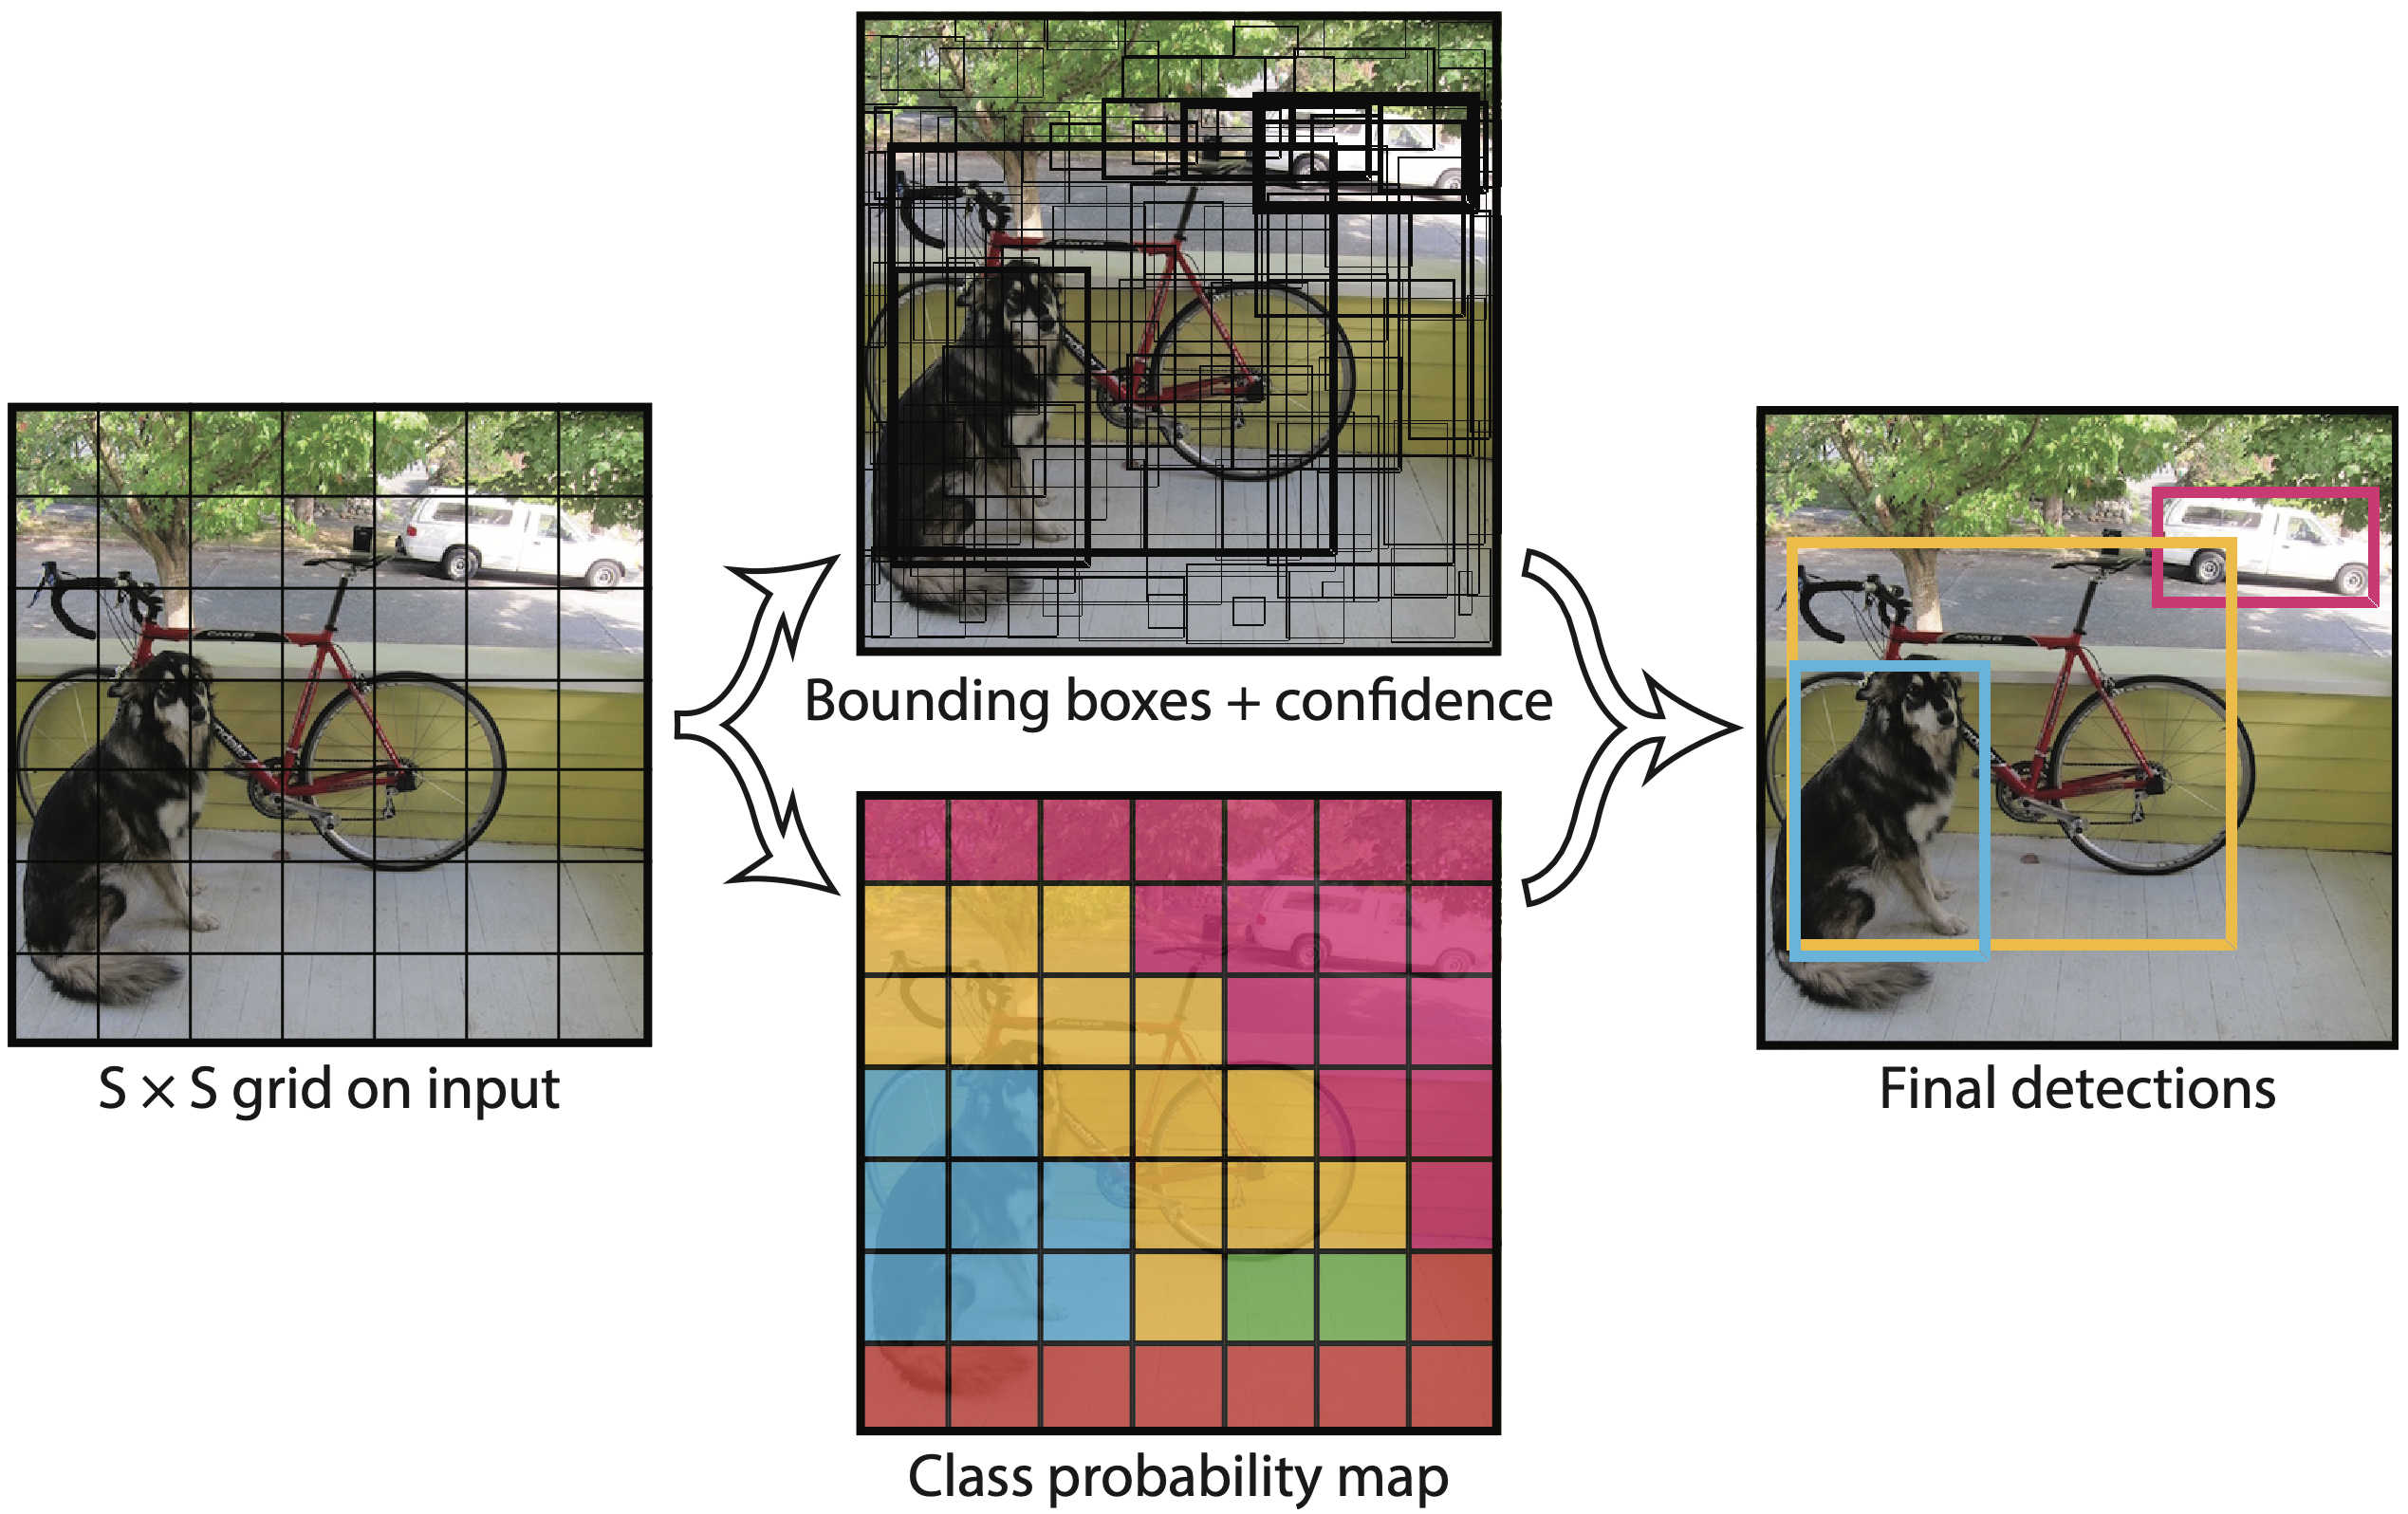
\includegraphics[width=\columnwidth]{images/yolo-model.png}
    \end{center}
    \caption{Pipeline of YOLO object detector: it divides the image into an $S \times S$ grid and for each grid cell predicts $B$ bounding boxes, confidence for those boxes, and $C$ class probabilities. These predictions are encoded as an $S \times S \times (B * 5 + C)$ tensor \cite{redmon2016you}.}
    \label{fig:yolo-model}
\end{figure}

In YOLO, the input image is divided into an $S \times S$ grid and the cell in which the center of the object falls is responsible for the detection of that object.
A grid cell can predict more than one bounding box, where each prediction consists of an array composed by 5 elements: center of the bounding box identified by the coordinates $x$ and $y$, dimensions of the box $w$ and $h$, and the confidence score of that bounding box representing an object. At the same time, regardless of the number of boxes in each cell, $C$ conditional probabilities $\Pr(Class_i | Object)$ are computed in each grid cell. The final prediction will be encoded as an $S \times S \times (B * 5 + C)$ tensor. The model pipeline is shown in \autoref{fig:yolo-model}.

In order to predict and localize many different objects in an image, YOLO uses anchor boxes, which are a set of predefined bounding boxes of a certain height and width. These boxes are defined to capture the scale and aspect ratio of specific object classes. Then, the predefined anchor boxes are used as a starting point during detection.

The model is trained via the optimization of the following loss function:

\begin{equation}\label{eq:yolo-loss}
    \begin{split}
        \mathcal{L} \quad =  \quad  &
            \lambda_{coord} \sum_{i=0}^{S^2} \sum_{j=0}^{B} \mathbb{1}_{ij}^{obj}
            [(x_i - \hat x_i)^2 + (y_i - \hat y_i)^2]\\
            \quad + \quad & \lambda_{coord} \sum_{i=0}^{S^2} \sum_{j=0}^{B} \mathbb{1}_{ij}^{obj}
                [(\sqrt{w_i} - \sqrt{\hat w_i})^2 + (\sqrt{h_i} - \sqrt{\hat h_i})^2]\\
            \quad + \quad & \sum_{i=0}^{S^2} \sum_{j=0}^{B} \mathbb{1}_{ij}^{obj}
                (C_i - \hat C_i)^2 \; + \; \lambda_{noobj} \sum_{i=0}^{S^2} \sum_{j=0}^{B} \mathbb{1}_{ij}^{noobj}(C_i - \hat C_i)^2\\
            \quad + \quad & \sum_{i=0}^{S^2} \mathbb{1}_{i}^{obj} \sum_{c \in classes}
                (p_i(c) - \hat p_i (c))^2\\
    \end{split}
\end{equation}
where,
\begin{align*}
    \mathbb{1}_{ij}&=\left\{
        \begin{array}{@{}ll@{}}
            1, & \text{if the } j \text{-th bbox in cell } i \text{ is responsible for that prediction}\\
            0, & \text{otherwise}
        \end{array}\right.\\
    \mathbb{1}_{i}&=\left\{
        \begin{array}{@{}ll@{}}
            1, & \text{if there is an object in cell}\ i \\
            0, & \text{otherwise}
        \end{array}\right.
\end{align*}


The loss function in \autoref{eq:yolo-loss} considers both detection and classification. A bounding box can be defined by its center in addition to the height and width. The first row of the loss function is responsible for minimizing the difference between the predicted center and the ground truth, and the second row minimize the difference between width and height.
The third row penalizes the neural network if it predicts an object whereas it is not present and vice versa. The last row of the loss function is the mean squared error between the real class and the predicted one, hence it is responsible to match the real class.


Over the years, several versions of YOLO have come up, starting from the first up to fifth version \cite{redmon2016you, redmon2017yolo9000, redmon2018yolov3, bochkovskiy2020yolov4, glenn_jocher_2021_5563715}. YOLOv5 represents the state of the art for object detection, and compared with the most recent models it is among the best performing ones \cite{zaidi2022survey}.

\section{Logo recognition}
\label{sec:sota-logoyolo}

A general pipeline for logo detection and recognition consists in logo region proposal followed by a classifier specifically trained for logo classification, as proposed by Bianco et al. in \cite{bianco2017deep} or by Fehérvári et al. in \cite{fehervari2019scalable}.

Another approach presented by Wang et al. \cite{wang2022logodet} involves a model based on YOLOv3 \cite{redmon2018yolov3} used to produce both bounding boxes and classification for each detected logo. The proposed model is called Logo-YOLO, which is essentially the same version of YOLOv3 with some changes to the loss function described in \autoref{eq:yolo-loss} and the re-computation of the anchors sizes. The modified loss function utilizes the Focal Loss \cite{lin2017focal} to solve the problem of the logos which are small objects to the background, and the  CIoU loss \cite{zheng2020distance} to obtain more accurate and faster regression of the bounding boxes.

The issue with these approaches is the closed-world assumption which does not apply in the case of logo recognition, as discussed in \autoref{sec:logodet-intro}. This is the purpose behind works such as \cite{fehervari2019scalable}. The authors of the paper propose a method based on Distance Metric Learning (DML) using deep learning techniques called SoftTriple Loss presented in \cite{qian2019softtriple}. This work aims to achieve logo recognition via metric learning, where a model learns the similarity of different objects in a latent space, thus being able to deal with a large number of previously unseen classes exploiting the distances of objects in the latent space.

Another work based on DML has been presented by Li et al. \cite{li2022seetek} and can be considered as an extension to \cite{fehervari2019scalable}. In this work the authors enrich the latent space learned by DML with text features contained in the logos. The authors highlight how a large number of logos have remarkable amount of text or (stylized) letters, for this reason, in addition to visual features, they consider text features as relevant information for logo classification.

\section{Class incremental learning}
Traditional supervised learning systems are trained in closed-world for a fixed
number of classes, that requires all the training data to be available before training.
The problem of Class Incremental Learning (CIL) aims to design algorithms that can learn new concepts in a sequential way and eventually perform well on all observed classes \cite{yan2021dynamically}.

To extend a trained model on new classes, a large amount of labeled data for both new
and old classes is necessary for network finetuning. Otherwise, if the dataset of old classes is no
longer available, finetuning a deployed model with
new classes can lead to the catastrophic forgetting
problem \cite{serra2018overcoming, zhang2021few, mccloskey1989catastrophic}. Catastrophic forgetting means that a model degrades performance on old classes when retrained on new ones.

\subsection{Problem setup}


\begin{figure}
    \begin{center}
        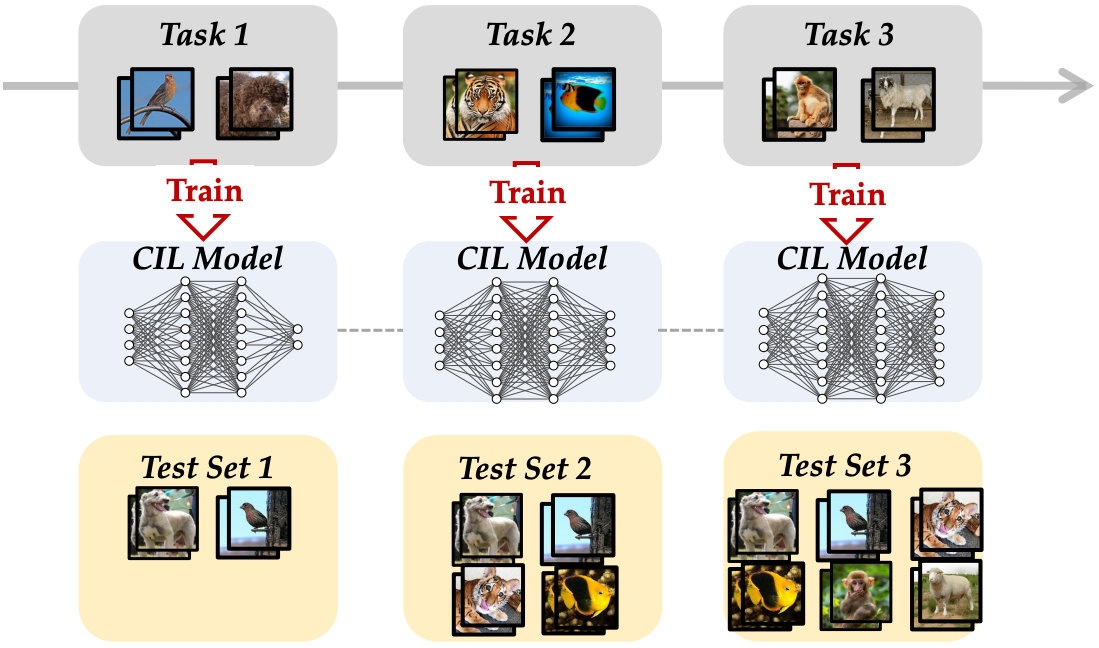
\includegraphics[width=0.9\columnwidth]{images/cil-setup.png}
    \end{center}
    \caption{General CIL setup. In an incremental learning setup, classes arrive sequentially at each task, so we only have access to the classes of that task and the previously seen classes. To classify new classes using the same model, the classifier is built incrementally. After the learning stage of each task, the model
    is evaluated among all seen classes. The image shows an example of three incremental learning steps. Image from \cite{zhou2021pycil}.}
    \label{fig:cil-setup}
\end{figure}

During CIL, a stream of class groups $\{\mathcal{Y}_t\}$ and their corresponding training data $\{\mathcal{D}_t\}$ are observed by the model. At step $t$, the incoming dataset $\{\mathcal{D}_t\}$ is of the form $(\textbf{x}_{\textbf{i}}^{\textbf{i}}, y_i^t)$ where $\textbf{x}_{\textbf{i}}^{\textbf{i}}$ is the input image and $y_i^t \in \mathcal{Y}_t$ is the label set $\mathcal{Y}_t$. The label space of the model consists in all the seen categories $\tilde{\mathcal{Y}}_t = \cup_{i=1}^t \mathcal{Y}_i$ and a good model should predict well on all classes $\tilde{\mathcal{Y}}_t$. As described in \autoref{sec:cil-methods}, some CIL algorithms save a part of data at timestamp $t$ as the memory $\mathcal{M}_t$ for future training. The CIL setup is shown in \autoref{fig:cil-setup}.

\subsection{Methods}
\label{sec:pycil}
\label{sec:cil-methods}


\begin{figure}
    \centerline{
        \begin{forest} for tree={align=center, inner sep=2pt}
        [Class Incremental Learning (CIL)\\methods
        [Replay\\methods
            [Rehearsal
            [
                iCaRL \cite{rebuffi2017icarl}\\
                ER \cite{rolnick2019experience}\\
                SER \cite{isele2018selective}\\
                TEM \cite{chaudhry2019continual}\\
                CoPE \cite{de2021continual}
            ]
            ]
            [Pseudo\\Rehearsal
            [
                DGR \cite{shin2017continual}\\
                PR \cite{atkinson1802pseudo}\\
                CCLUGM \cite{lavda2018continual}\\
                LGM \cite{ramapuram2020lifelong}\\
            ]
            ] 
            [Constrained
            [
                GEM \cite{lopez2017gradient}\\
                A-GEM \cite{chaudhry2018efficient}\\
                GSS \cite{aljundi2019online}\\
            ]
            ] 
        ]
        [Regularization-based\\methods
        [Prior-focused 
            [
                EWC \cite{kirkpatrick2017overcoming}\\
                IMM \cite{lee2017overcoming}\\
                SI \cite{zenke2017continual}\\
                R-EWC \cite{liu2018rotate}\\
                MAS \cite{aljundi2018memory}\\
                Riemannian Walk \cite{chaudhry2018riemannian}\\
            ]
        ]
        [Data-focused 
            [
            LwF \cite{li2017learning}\\
            LFL \cite{jung2016less}\\
            EBLL \cite{rannen2017encoder}\\
            DMC \cite{zhang2020class}\\
            ]
        ]
        ]
        [Parameter\\isolation methods
        [Fixed\\Network
            [
                PackNet \cite{mallya2018packnet}\\
                PathNet \cite{fernando2017pathnet}\\
                Piggybak \cite{mallya2018piggyback}\\
                HAT \cite{serra2018overcoming}\\
            ]
        ]
        [Dynamic\\Network
            [
                PNN \cite{rusu2016progressive}\\
                Expert Gate \cite{aljundi2017expert}\\
                RCL \cite{xu2018reinforced}\\
                DAN \cite{rosenfeld2018incremental}\\
            ]    
        ]]
        ]
        \end{forest}
    }
    \caption{CIL algorithms taxonomy presented in \cite{delange2021continual}.}
    \label{fig:cil-taxonomy}

\end{figure}


     

The problem of CIL has been addressed using different methods, and they can be divided into three main categories and their sub-categories. The taxonomy and the list of algorithms, summarized in the \autoref{fig:cil-taxonomy}, is based on these works \cite{liu2021adaptive, delange2021continual}:

 

\begin{enumerate}
    \item \textbf{Replay methods}: these works store samples of old classes which are replayed while learning a new task, by doing so it is possible to alleviate forgetting.
    The samples are either reused as model inputs for rehearsal, or to constrain the optimization of loss on the new tasks.

    \begin{enumerate}
        \item \textit{Rehearsal} \cite{rebuffi2017icarl, rolnick2019experience, isele2018selective, chaudhry2019continual, de2021continual}: the model is retrained on a limited subset of stored samples.
        \item \textit{Pseudo Rehearsal} \cite{shin2017continual, atkinson1802pseudo, lavda2018continual, ramapuram2020lifelong}: approximates previous tasks samples using either random input vector or more advanced techniques like generative models. However, the latter one has the drawback of adding complexity to the system pipeline.
        \item \textit{Constrained optimization} \cite{lopez2017gradient, chaudhry2018efficient, aljundi2019online}: updates the model weights for the new task in such a way as not to interfere with previous task weights.
    \end{enumerate}
    
    \item \textbf{Regularization-based methods}: these works do not store raw data and reduce the memory requirements. An extra regularization term is introduced in the loss function, in this way it is possible to learn new classes while maintaining the previous knowledge.
    \begin{enumerate}
        \item \textit{Prior-focused methods} \cite{kirkpatrick2017overcoming, lee2017overcoming, zenke2017continual, liu2018rotate, aljundi2018memory, chaudhry2018riemannian}: this approach tries to estimate the importance of the neural network parameters to avoid forgetting as much as possible. Then, when training on new tasks, the optimization process penalizes changes to important weights.
        \item \textit{Data-focused methods} \cite{li2017learning, jung2016less, zhang2020class, rannen2017encoder}: this approach uses knowledge distillation \cite{hinton2015distilling} treating the old model trained on the previous task as the \textit{teacher}, and use it combined with the new data to train the \textit{student} model.
    \end{enumerate}
    \item \textbf{Parameter isolation methods}: this class of methods use different model parameters for each task.
    \begin{enumerate}
        \item \textit{Fixed Network} \cite{mallya2018packnet, mallya2018piggyback, serra2018overcoming, fernando2017pathnet}: the model architecture is kept fixed and the knowledge is updated involving masks for the parameters' weights.
        \item \textit{Dynamic Architectures} \cite{rusu2016progressive, xu2018reinforced, aljundi2017expert, rosenfeld2018incremental}: the model architecture dynamically changes after each incremental task, and the old parameters are frozen to prevent forgetting. Another approach is to dedicate a model to each incremental task.
    \end{enumerate}
\end{enumerate}

Since there are several different algorithms for CIL, the work presented by Zhou et al. in \cite{zhou2021pycil} aims to compare a subset of these algorithms considering the same experimental setup. To this purpose, they publish a repository\footnote{PyCIL GitHub repository: \href{https://github.com/G-U-N/PyCIL}{https://github.com/G-U-N/PyCIL}}
on GitHub where they introduce \textit{PyCIL: A Python Toolbox for Class-Incremental Learning}, which is an implementation of all the following algorithms:

\begin{itemize}
    \item \textbf{Finetune}: the baseline method which updates parameters on new tasks and
    suffers from severe catastrophic forgetting.
    \item \textbf{Replay}: the baseline method which updates parameters on new task with instances
    from the new dataset and exemplar set.
    \item \textbf{EWC} \cite{kirkpatrick2017overcoming}: uses Fisher Information Matrix to weigh the
    importance of each parameter and regularizes important parameters to overcome forgetting.
    \item \textbf{LwF} \cite{li2017learning}: uses knowledge distillation \cite{hinton2015distilling} to
    align the output probability between old and new model.
    \item \textbf{iCaRL} \cite{rebuffi2017icarl}: uses knowledge distillation  \cite{hinton2015distilling}  to
    align the output probability between old and new model. Moreover, it also introduces
    exemplar set for rehearsal and uses nearest center mean classifier.
    \item \textbf{GEM} \cite{lopez2017gradient}: uses exemplars as the regularization of
    gradient updating.
    \item \textbf{BiC} \cite{wu2019large}: trains an extra adaptation layer based on iCaRL, which
    adjusts the logits on new classes.
    \item \textbf{WA} \cite{zhao2020maintaining}: normalizes the classifier weight after each learning session
    based on iCaRL.
    \item \textbf{PODNet} \cite{douillard2020podnet}: introduces a novel distillation loss (Pooled
    Outputs Distillation) constraining the whole convolutional network.
    \item \textbf{DER} \cite{yan2021dynamically}: a two-stage learning approach that utilizes a dynamically
    expandable representation for more effective incremental concept modeling.
    \item \textbf{Coil} \cite{zhou2021co}: builds bi-directional knowledge transfer in the class incremental learning process with optimal transport \cite{villani2009optimal}. It first addresses
    the ability that old model can help learning new classes.
\end{itemize}

The CIL algorithms are tested on two different benchmark datasets, i.e. CIFAR100 \cite{krizhevsky2009learning} and ImageNet100 \cite{russakovsky2015imagenet}. These datasets are composed of 100 classes and the experiments performed in PyCIL \cite{zhou2021pycil} adopt this CIL setup: 10 classes for the initial stage followed by 9 incremental learning iterations consisting of 10 new classes. Then, the top-1 accuracy is reported for all the incremental stages.
The results are shown in \autoref{fig:cil-comaprison} and the top-1 accuracy at the final stage is reported in \autoref{table:cil-results}.

\begin{figure}%
	\centering
	\subfloat[\centering 10 stage on CIFAR100]{{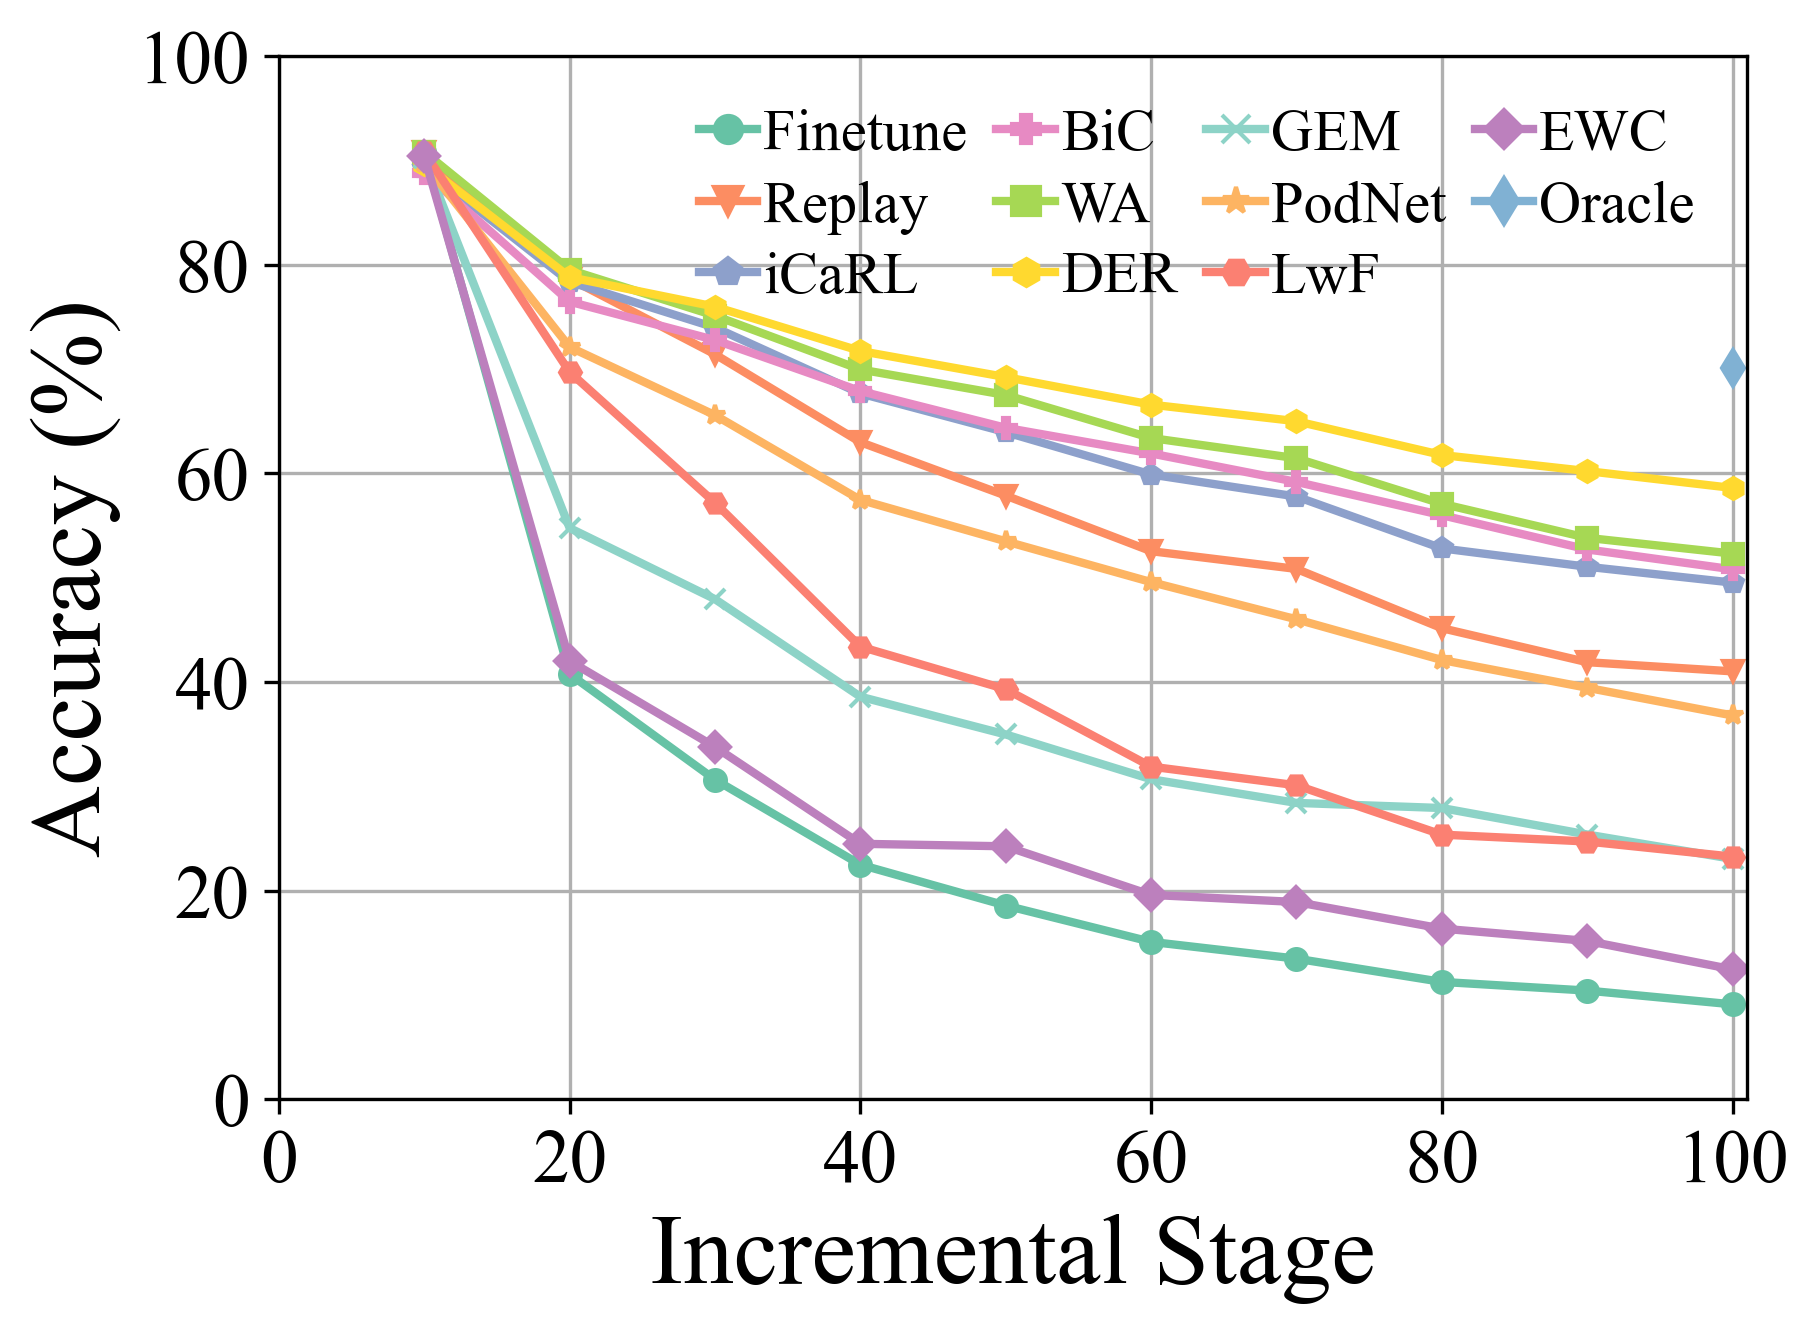
\includegraphics[width=0.45\textwidth]{images/cil-cifar.png} }}%
	\hfill
	\subfloat[\centering 10 stage on ImageNet100]{{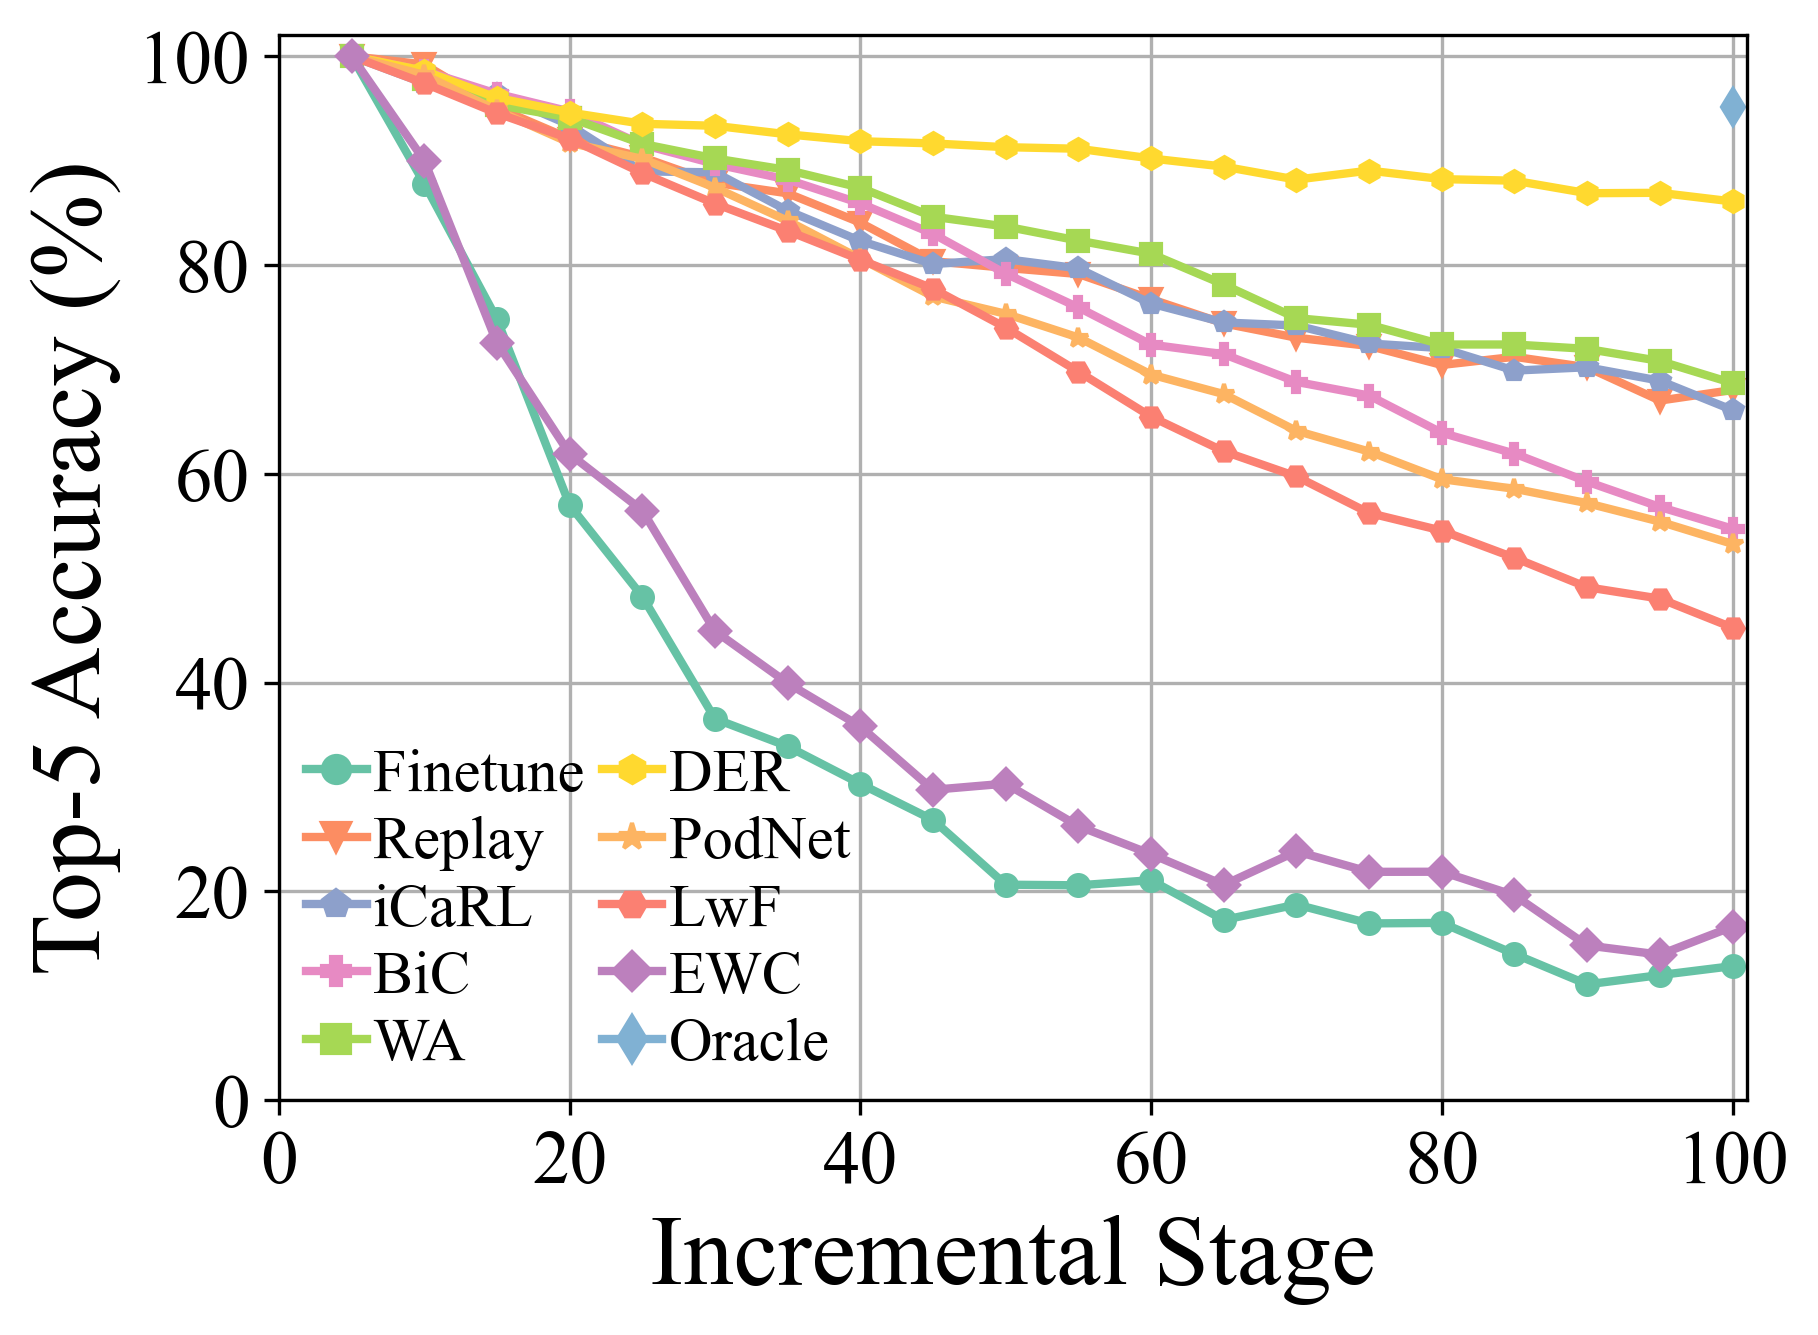
\includegraphics[width=0.45\textwidth]{images/cil-imagenet} }}%
	\caption{Performance comparison of the CIL algorithms during 10 stages on CIFAR100 and ImageNet100 datasets \cite{zhou2021pycil}.}%
	\label{fig:cil-comaprison}%
\end{figure}

\begin{table}
    \centering
    \begin{tabular}{c c c} 
     \hline
     \textbf{Method} & \textbf{Reproduced} & \textbf{Reported} \\
     & \textbf{in PyCIL}\\
     \hline
     \hline
     Finetune & 26.25& 26.25 \\

    Replay & 59.31 & - \\ 

    GEM & 40.18 & - \\ 

    LwF & 43.56 & - \\ 

    iCaRL & 64.42 & 64.10 \\ 

    EWC & 29.73 & - \\ 

    WA & 67.09 & 64.5 \\ 

    PODNet & 55.22 & - \\ 

    BiC & 65.08 & - \\ 

    Coil & 65.48 & 65.48 \\ 

    DER & 69.74 & 69.41 \\ 
    \hline
    \end{tabular}
    \caption{Top-1 accuracy of the CIL algorithms at the $10$-th incremental stage using the CIFAR100 dataset \cite{zhou2021pycil}.}
    \label{table:cil-results}
    \end{table}

From the final results reported in PyCIL in \autoref{table:cil-results} it is clear that the best performing algorithm on the considered datasets is DER \cite{yan2021dynamically}. Moreover, even if the authors of PyCIL re-implement the DER algorithm, they point out how the performance obtained from the implementation of PyCIL is very similar to that reported in the original DER paper (69.74 top-1 accuracy in PyCIL vs 69.41 reported by the DER paper).


\subsection{DER: an algorithm for class incremental learning}
\label{sec:der-algorithm}
DER (dynamically expandable representation) is an algorithm for CIL based on a two-stage learning approach that utilizes a dynamically expandable representation and uses a limited memory for the old classes introduced in each incremental step. The system proposed in this thesis takes advantage of this algorithm for what concerns the incremental learning aspect of the classifier (see \autoref{sec:method-classifier}).


\begin{figure}%
	\centering

    \begin{center}
        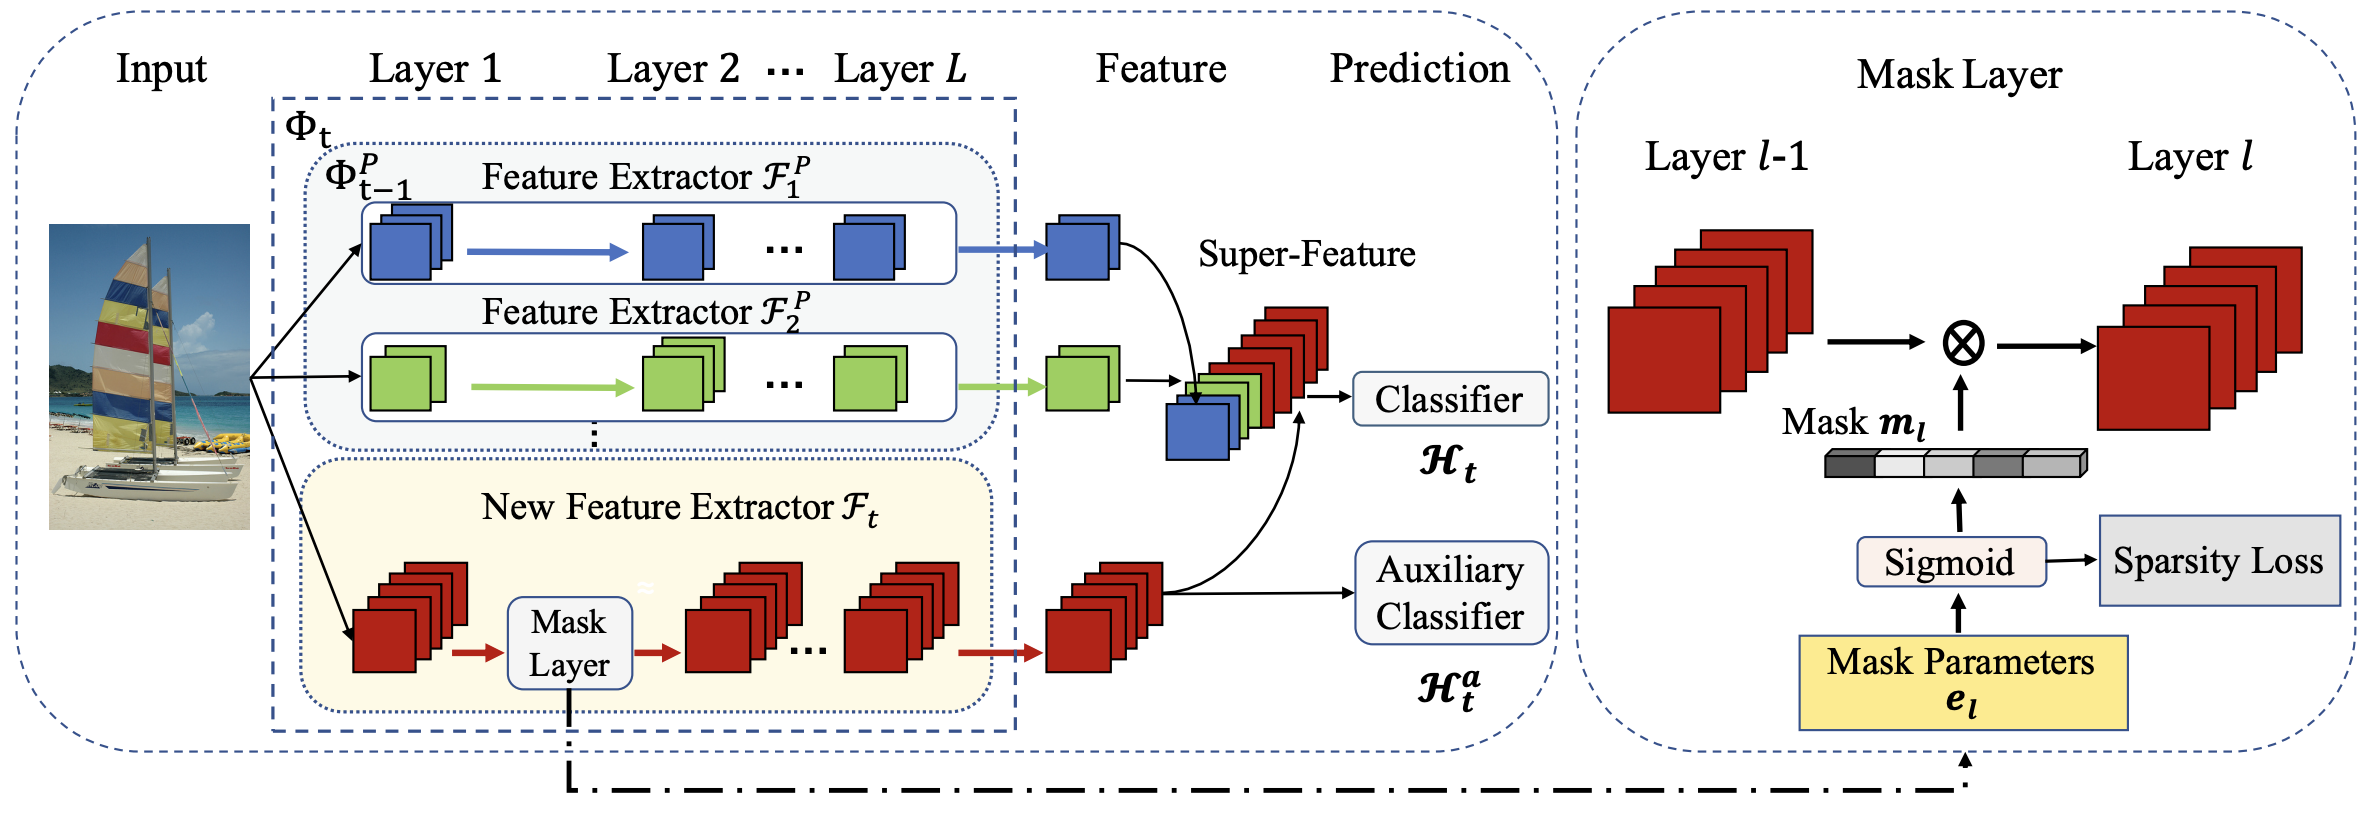
\includegraphics[width=\columnwidth]{images/der-pipeline.png}
    \end{center}

	\caption{Dynamically Expandable Representation Learning method: at step $t$, the model is composed of the super-feature extractor $\Phi_t$ and the classifier $\mathcal{H}_t$. $\Phi_t$ is created using the previous super-feature extractor $\Phi_{t-1}$ and the newly created feature extractor $\mathcal{F}_t$. An auxiliary classifier $\mathcal{H}_t^a$ is introduced to regularize the model. Moreover, a channel-level
    mask-based pruning strategy is used to maintain a compact representation of the model \cite{yan2021dynamically}.}%
	\label{fig:der-pipeline}%
\end{figure}


The DER algorithm described in \cite{yan2021dynamically} can be divided into three stages (see \autoref{fig:der-pipeline}):
\begin{enumerate}
    \item \textbf{Representation Learning Stage}: the architecture of the Convolutional Neural Network (CNN) is dynamically expanded at each new incremental learning iteration.
    \item \textbf{Masking and Pruning}: the CNN introduced in the last incremental learning stage is pruned using a channel-level masked-based method.
    \item \textbf{Classifier Learning Stage}: retrain the classifier with currently available data $\tilde{\mathcal{D}}_t = \mathcal{D}_t \cup \mathcal{M}_t$ at step $t$.
\end{enumerate}

\subsubsection{Expandable Representation Learning}
At step $t$ of the incremental learning, the algorithm defines a super-feature extractor $\Phi_t$ and the classifier $\mathcal{H}_t$. The algorithm expands the neural network architecture at each step by considering the previous super-feature extractor $\Phi_{t-1}$ and a newly created feature extractor $\mathcal{F}_t$. The feature extractor $\mathcal{F}_t$ consists of a CNN, and the classifier $\mathcal{H}_t$ is a Fully Connected (FC) layer after the super-feature extractor $\Phi_t$.

Given an image $\textbf{x} \in \tilde{\mathcal{D}}_t$, the feature $u$ extracted by $\Phi_t$ is the result of the following concatenation:
\begin{equation}
    \textbf{u} = \Phi_t(\textbf{x}) = [\Phi_{t-1}(\textbf{x}), \mathcal{F}_t(\mathbf{x})]
\end{equation}
The feature $\textbf{u}$ is then fed into the classifier $\mathcal{H}_t$, which is defined in such a way that the input and output dimensions for step $t$ match. Then, the prediction is produced as follows:
\begin{equation} \label{eq:classification}
    p_{\mathcal{H}_t}(\textbf{y} | \textbf{x}) = \text{Softmax}(\mathcal{H}_t(\textbf{u}))
\end{equation}
Finally, the actual predicted class is given by:
\begin{equation}
    \hat{y} = \argmax \mathcal{H}_t(\textbf{y} | \textbf{x}), \quad \hat{y} \in \tilde{\mathcal{Y}}_t
\end{equation}
The stability-plasticity tradeoff is taken into account considering these two aspects:
\begin{itemize}
    \item To \textbf{retain old knowledge}, the parameters of $\mathcal{H}_t$ for the old features are inherited from $\mathcal{H}_{t-1}$, and its newly added parameters are randomly initialized.
    \item To \textbf{reduce catastrophic forgetting}, the parameters $\theta_{\Phi_{t-1}}$ and the statistics of Batch Normalization \cite{ioffe2015batch} of the old super-feature extractor $\Phi_{t-1}$ are frozen at step $t$, in this way it is possible to maintain the previously learned knowledge.
\end{itemize}


To force the network to learn new and discriminative features at each incremental step, the authors of the algorithm introduce an auxiliary classifier $\mathcal{H}_t^a$. The label space of $\mathcal{H}_t^a$ is $|\mathcal{Y}_t| + 1$, corresponding to the the set $\mathcal{Y}_t$ of all new categories, and treating all the old concepts as a single category. This is done to encourage the network to learn features that discriminate old and new concepts. The classifier $\mathcal{H}_t^a$ predicts the probability:
\begin{equation} \label{eq:loss-aux}
    p_{\mathcal{H}_t^a}(\textbf{y}|\textbf{x}) = \text{Softmax}(\mathcal{H}_t^a(\mathcal{F}(\textbf{x})))
\end{equation}

\subsubsection{Masking and pruning}
\label{sec:masking-pruning}
To maintain a compact representation of the model and remove redundancy, the super-feature extractor is pruned after the training of each stage $t$, the method proposed by the authors is adapted from \cite{serra2018overcoming}. This is done using a differentiable channel-level mask-based method to prune filters of the extractor $\mathcal{F}_t$, in which
the masks are learned jointly with the representation. The mask is then binarized after the learning procedure, and the feature extractor $\mathcal{F}_t$ is pruned using the binary mask, producing as output the pruned network $\mathcal{F}_t^{P}$.

Given a new feature extractor $\mathcal{F}_t$, the input feature map of the convolutional layer $l$ for an image $\textbf{x}$ is denoted as $\textbf{f}_l$. The channel mask $\textbf{m}_l \in \mathbb{R}^{c_l}$ controls the size of the layer $l$, where $m_l^i \in [0, 1]$ and $c_l$ is the number of channels of layer $l$. The mask $m_l$ is used to modulate $f_l$ as follows:

\begin{equation}
    \textbf{f}_l \kern 0.05em ' = \textbf{f}_l \odot \textbf{m}_l
\end{equation}
where $\textbf{f}_l \kern 0.05em '$ is the masked feature map and $\odot$ means channel-level multiplication. To make the values of $\textbf{m}_l$ fall into the interval $[0,1]$, the mask is given by:
\begin{equation}\label{eq:mask}
    \textbf{m}_l = \sigma(s \textbf{e}_l)
\end{equation}
where $\textbf{e}_l$ is the learnable mask parameters, $\sigma(\cdot)$ is the sigmoid used as gating function, and $s$ is a scaling factor to control the sharpness of the function.


Using the pruning mechanism, the super-feature $\tilde{\textbf{u}}$ of step $t$ can be rewritten as:
\begin{equation}
    \tilde{\textbf{u}} = \Phi_t^P(\textbf{x}) = [\mathcal{F}_1^P, \mathcal{F}_2^P,\, ..., \phi(\textbf{x})]
\end{equation}

During the training $\phi_t(\textbf{x})$ corresponds to $\mathcal{F}_t(\textbf{x})$ with the soft mask. At inference time, thanks to the scaling factor $s$, the masks associated to the filters of the convolutional layers are pruned assigning a large value to $s$. In this way it is possible to obtain $\mathcal{F}_t^P = \phi_t(\textbf{x})$.

The parameters $\textbf{e}_l$ which define the masks are learned during training. During an epoch, a linear annealing schedule is applied for scaling factor $s$ as follows:
\begin{equation}
    s = \frac{1}{s_{max}} + (s_{max}- \frac{1}{s_{max}}) \frac{b-1}{B-1}
\end{equation}
where $b$ is the batch index, $B$ is the number of batches in one epoch, and $s_{max} \gg 1$ is a hyperparameter.

In this way, at the start of the training epoch, $s$ has a small value. Thus, given that $\textbf{m}_l=\sigma(s \textbf{e}_l)$, the gating mechanism leads to values close to $0.5$, regardless of the $\textbf{e}_l$ vector. Then the mask is progressively binarized with the increasing of the batch index $b$ within a epoch.

As described in \cite{serra2018overcoming}, to solve the problem of the unstable gradient of $\textbf{e}_l$ due to the $s$ schedule, the gradient $\textbf{g}_{\textbf{e}_l}$ with respect to $\textbf{e}_l$ is compensated as follows:
\begin{equation}
    \textbf{g}_{\textbf{e}_l} ' = \frac{\sigma(\textbf{e}_l)[1-\sigma(\textbf{e}_l)]}{s\sigma(s\textbf{e}_l)[1-\sigma(s\textbf{e}_l)]}\textbf{g}_{\textbf{e}_l}
\end{equation}
where $\textbf{g}_{\textbf{e}_l} '$ is the compensated gradient.


\subsubsection{Classifier Learning}
After the representation learning stage, the classifier head is re-trained to reduce the bias in the classifier weight introduced by the imbalanced training set $\tilde{\mathcal{D}}_t$, this is due to the difference in sample size between the old classes in the memory $\mathcal{M}_t$ and the currently available data $\mathcal{D}_t$. To this purpose, the classifier weight are randomly initialized and the classifier is trained on a class-balanced sample of $\tilde{\mathcal{D}}_t$ using the cross-entropy loss with a temperature $\delta$ in the Softmax presented in \cite{zhao2020maintaining}. 

\subsubsection{Loss function}
The loss function used to change the parameters of the model is defined by three components:

\begin{enumerate}
    \item \textbf{Classifier Loss}: the first loss component is responsible for the correct classification of all the images. Hence, based on the \autoref{eq:classification}, given an image and its corresponding label $(\textbf{x}_i, y_i)\in \tilde{\mathcal{D}}$, the loss function penalizes wrong class prediction as follows:
    \begin{equation} \label{eq:loss1}
        \mathcal{L}_{\mathcal{H}_t} = - \frac{1}{|\tilde{\mathcal{D}}_t|}
            \sum_{i=1}^{|\tilde{\mathcal{D}}_t|}log(p_{\mathcal{H}_t}(y=y_i | \textbf{x}_i))
    \end{equation}
    \item \textbf{Auxiliary Loss}: the second loss component is relative to the auxiliary classifier $\mathcal{H}_t^a$. Consistently with \autoref{eq:loss-aux}, given an image $\textbf{x}_i$ and the associated label $y_i \in \mathcal{Y}_i \cup \{"old"\}$, the auxiliary loss component is defined as follows:
    \begin{equation} \label{eq:loss2}
        \mathcal{L}_{\mathcal{H}_t^a} = - \frac{1}{|\tilde{\mathcal{D}}_t|}
            \sum_{i=1}^{|\tilde{\mathcal{D}}_t|}log(p_{\mathcal{H}_t}(y=y_i | \textbf{x}_i))
    \end{equation}
    \item \textbf{Sparsity Loss}: the third loss component encourage the model to maximally reduce the number of parameters with a minimal performance drop. To this reason the sparsity loss considers the ratio of used weights in all available weights:
    \begin{equation} \label{eq:loss3}
        \mathcal{L}_S = \frac{\sum_{l=1}^L K_l \| \textbf{m}_{l-1} \|_1  \| \textbf{m}_{l} \|_1 }{\sum_{l=1}^L K_l c_{l-1} c_{l}}
    \end{equation}
    where $L$ is the number of layers and $K_l$ is the kernel size of convolutional layer $l$.
\end{enumerate}

The final loss function is given by the weighted average of \autoref{eq:loss1}, \autoref{eq:loss2} and \autoref{eq:loss3}:
\begin{equation}\label{eq:final_der_loss}
    \mathcal{L}_{DER} = \mathcal{L}_{\mathcal{H}_t} + \lambda_a \mathcal{L}_{\mathcal{H}_t^a} + \lambda_s \mathcal{L}_{S}
\end{equation}
where $\lambda_a$ and $\lambda_s$ are the hyper-parameter to control the effect of the auxiliary classifier and the pruning aspect.

\section{Weight aligning}
Weight aligning (WA) proposed in \cite{zhao2020maintaining} is a method to alleviate catastrophic forgetting in Deep Neural Networks (DNNs). In their work the authors show how a model trained for a CIL task tends
to classify objects into new classes, treating old classes unfairly. This is due to the weights
in the trained model's FC layer which are heavily biased. WA aims to correct bias in the FC layer.

\subsubsection{Biased Weights in the FC Layer}
\label{sec:wa-biased}
At the $t$-th incremental learning step, the model is given by:
\begin{equation}
    o(\textbf{x}) = \textbf{W}^T \Phi(\textbf{x})
\end{equation}
where:
\begin{itemize}
    \item $\Phi(\textbf{x})$ is the feature extractor which outputs a $d$-dimensional feature vector.
    \item $o(\textbf{x})$ is the ($C_{old}^t + C^t$)-dimensional vector of the logits produced in output by the model. $C_{old}^t$ and $C^t$ represent respectively the number of old and new classes at the $t$-th incremental stage. 
    \item $W \in \mathbb{R}^{d \times (C_{old}^t + C^t)}$ represents the parameters of the FC layer. $W$ can be espressed as $W = {w_c, \, 1 \leq c \leq C_{old}^b + C^b}$, where $w_c$ is a $d$-dimensional weight vector for the $c^{th}$ class.
\end{itemize}
The output logits for the $c^{th}$ class are calculated as:
\begin{equation}
    o_c(\textbf{x}) = \textbf{w}_c^T \Phi (\textbf{x})
\end{equation}
The motivation behind WA is the observation that the norms of weight vectors for new classes are larger, thus leading the output logits for new classes to be larger in general. As a result, the biased FC layer in the model tends to predict an input image as belonging to a new class. This analysis emerges from the experiments performed in \cite{zhao2020maintaining} shown in \autoref{fig:wa-biased}.
\begin{figure}%
    \hspace*{-1.25 cm}
	\subfloat[$C^0=20,C_{old}^0=0$]{{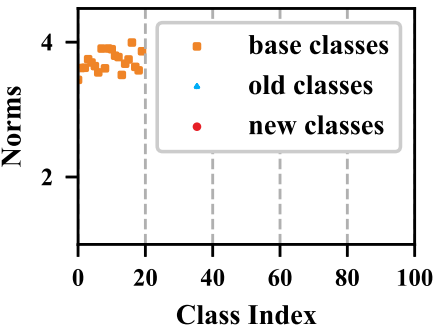
\includegraphics[width=0.22\textwidth]{images/wa-biased_1.png} }}
	\subfloat[$C^1=20,C_{old}^1=20$]{{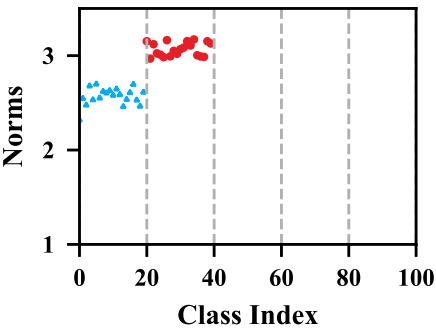
\includegraphics[width=0.22\textwidth]{images/wa-biased_2.png} }}
	\subfloat[$C^2=20,C_{old}^2=40$]{{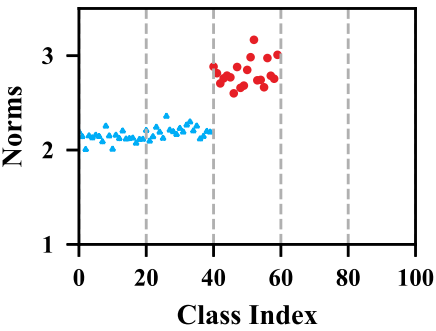
\includegraphics[width=0.22\textwidth]{images/wa-biased_3.png} }}
	\subfloat[$C^3=20,C_{old}^3=60$]{{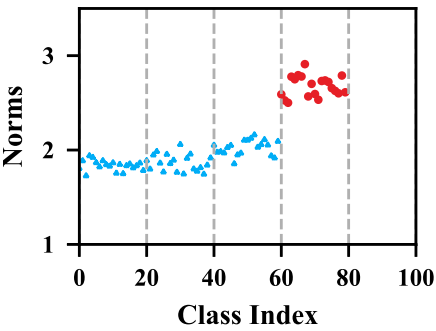
\includegraphics[width=0.22\textwidth]{images/wa-biased_4.png} }}
	\subfloat[$C^4=20,C_{old}^4=80$]{{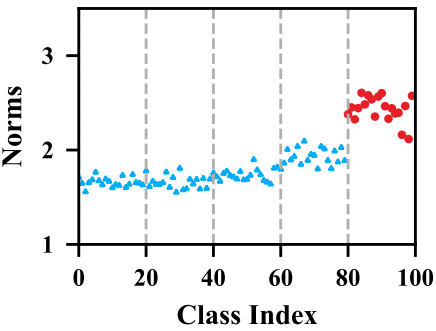
\includegraphics[width=0.22\textwidth]{images/wa-biased_5.png} }}
	\caption{Norm of the weight vectors $\{\textbf{w}_c\}$ after each incremental step. (a) Represents the initial step; (b), (c), (d), (e) are the $1^{st}$, $2^{nd}$, $3^{rd}$ and $4^{th}$ incremental step. The figure show the difference in the norms of the weight between the old and new classes \cite{zhao2020maintaining}.}%
	\label{fig:wa-biased}
\end{figure}

\subsubsection{Correct the biased weights in the FC Layer}
The bias in the weights of the FC layer described in \autoref{sec:wa-biased} is corrected using the WA tec.  The FC layer can be rewritten as $\textbf{W} = (\textbf{W}_{old}, \textbf{W}_{new})$, where 
$$\textbf{W}_{old} = (\textbf{w}_1, \textbf{w}_2, \, ..., \textbf{w}_{C_{old}^t}) \in \mathbb{R}^{d \times C_{old}^t},$$
$$\textbf{W}_{new} = (\textbf{w}_{C_{old}^t + 1}, \, ..., \textbf{w}_{C_{old}^t + C^t}) \in \mathbb{R}^{d \times C^t}.$$
The norms of the weight vectors of old and new classes can be denoted by:
$$\textbf{Norm}_{old} = (\| \textbf{w}_1 \|,  \, ..., \| \textbf{w}_{C_{old}^t \|}),$$
$$\textbf{Norm}_{new} = (\| \textbf{w}_{C_{old}^t + 1} \|, \, ..., \| \textbf{w}_{C_{old}^t + C^t} \|).$$
Then, the weights for new classes is normalized as follows:
\begin{equation}
    \hat{\textbf{W}}_{new} = \gamma \cdot \textbf{W}_{new}
\end{equation}
where
\begin{equation}
    \gamma = \frac{Mean(\textbf{Norm}_{old} )}{Mean(\textbf{Norm}_{new})}
\end{equation}
$Mean(\cdot)$ returns the mean value of elements in the vector.

This correction on the FC layer directly affects the output logits produced by the model. In fact, the output logits of the model before WA can be expressed as:
\begin{equation}
    \begin{split}
        \textbf{o}(\textbf{x}) = &\; (\textbf{o}_{old}(\textbf{x}), \textbf{o}_{new}(\textbf{x}))^T \\
        = &\; (\textbf{W}_{old}^T \Phi(\textbf{x}), \textbf{W}_{new}^T \Phi(\textbf{x}) )^T
    \end{split}
\end{equation}
after applying WA on the FC, the corrected output logits are given by:
\begin{equation}
    \begin{split}
        \textbf{o}_{corrected}(\textbf{x})
        = &\; (\textbf{W}_{old}^T \Phi(\textbf{x}), \hat{\textbf{W}}_{new}^T \Phi(\textbf{x}))^T \\
        = &\; (\textbf{W}_{old}^T \Phi(\textbf{x}), \gamma \cdot \textbf{W}_{new}^T \Phi(\textbf{x}))^T \\
        = &\; (\textbf{o}_{old}(\textbf{x}), \gamma \cdot \textbf{o}_{new}(\textbf{x}))^T
    \end{split}
\end{equation}

The final effect of aligning the weights is to rescale the output logits of new classes, thus leading to a fair classification between old and new classes.
\chapter{Dataset}
\label{chap:dataset}

A crucial part in the development of deep learning model is the dataset used for training. There are several datasets proposed in the literature for logo detection and recognition, however, some of them like BelgaLogos \cite{neumann2002integration} lack of variety in the number of classes and have a small number of images. For this reason, some works aimed to construct some larger dataset, such as \textit{WebLogo-2M} \cite{su2017weblogo} or \textit{Logos in the wild} \cite{tuzko2017open}. The issue with these types of large scale dataset is that they are automatically collected and labeled, leading to some noise in the target label.

A list of datasets proposed in the literature is given by Li et al. in SeeTek \cite{li2022seetek}, shown in \autoref{table:logo-datasets}.

\begin{table}
    \begin{center}
        \begin{tabular}{c || c | c | c | c | c |c} 
            \hline
            \textbf{Dataset} & \textbf{Logos} & \textbf{Images} & \textbf{Annotation} & \textbf{Noisy} & \textbf{Public} & \textbf{Scalability} \\
            \hline
            \hline
            TopLogo-10 \cite{su2017deep} & 10 & 700 & Object-Level & no & yes & Weak \\ 
       \hline
           BelgaLogos \cite{joly2009logo} & 37 & 10,000 & Object-Level & no & yes & Weak \\ 
       \hline
           FlickrLogos-32 \cite{romberg2011scalable} & 32 & 8,240 & Object-Level & no & yes & Weak \\ 
       \hline
           FlickrLogos-47 \cite{romberg2011scalable} & 47 & 8,240 & Object-Level & no & yes & Weak \\ 
       \hline
           Logo-NET \cite{hoi2015logo} & 160 & 73,414 & Object-Level & no & yes & Weak \\ 
       \hline
           WebLogo-2M \cite{su2017weblogo} & 194 & 2,190,757 & Image-Level & yes & yes & Medium \\ 
       \hline
           QMUL-OpenLogo \cite{su2018open} & 352 & 27,083 & Image-Level & no & yes & Medium \\ 
       \hline
           Logos in the wild \cite{tuzko2017open} & 871 & 11,054 & Object-Level & yes & yes & Medium \\ 
       \hline
           BLAC \cite{bastan2019large} & 2,800 & 6,200 & Object-Level & no & no & Medium \\ 
       \hline
           LogoDet-3K \cite{wang2022logodet} & 3,000 & 158,652 & Object-Level & no & yes & Strong \\ 
       \hline
           PL8K \cite{li2022seetek} & 7,888 & 3,017,146 & Object-Level & no & no & Strong \\ 
           \hline
       
           \end{tabular}
    \end{center}
    
    \caption{Statistics and characteristics of existing logo detection datasets \cite{li2022seetek}.}
    \label{table:logo-datasets}
\end{table}

Some logos datasets like LogoDet-3K and PL8K are considered more robust for what concern the image annotation (noisy column in \autoref{table:logo-datasets}). In particular, each image of LogoDet-3K is manually examined and
reviewed, this guarantees high-quality annotations.

In the face of this, the only two large-scale and non-noisy datasets of \autoref{table:logo-datasets} are LogoDet-3K and PL8K. However, only LogoDet-3K is publicly available, thus being the only viable choice as the target dataset to use for the experiments of this thesis (see \autoref{chap:experiments}).


\section{LogoDet-3K: dataset description}
LogoDet-3K consists of 3,000 logo classes,
158,652 images and 194,261 logo objects. The dataset is divided into nine categories, each category contains several brand and for each brand there is a set of images of that brand. The \autoref{table:logodet3k-category-statistics} shows the number of brands, images and objects for each category. it is important to point out how an image can contain multiple logo objects and the objects in the same image are not necessary of the same class (brand).


In this context, brand is intended as logo class. In fact, the same brand can have multiple versions of logos, for example, a symbolic logo and a textual logo. These type of logos are treaded as different classes in the LogoDet-3K dataset, a suffix such as '\textit{brand}-1' and '\textit{brand}-2' is used to deal with these cases. An example is given in \autoref{fig:logos-suffix}


\begin{figure}%
	\centering

    \begin{center}
        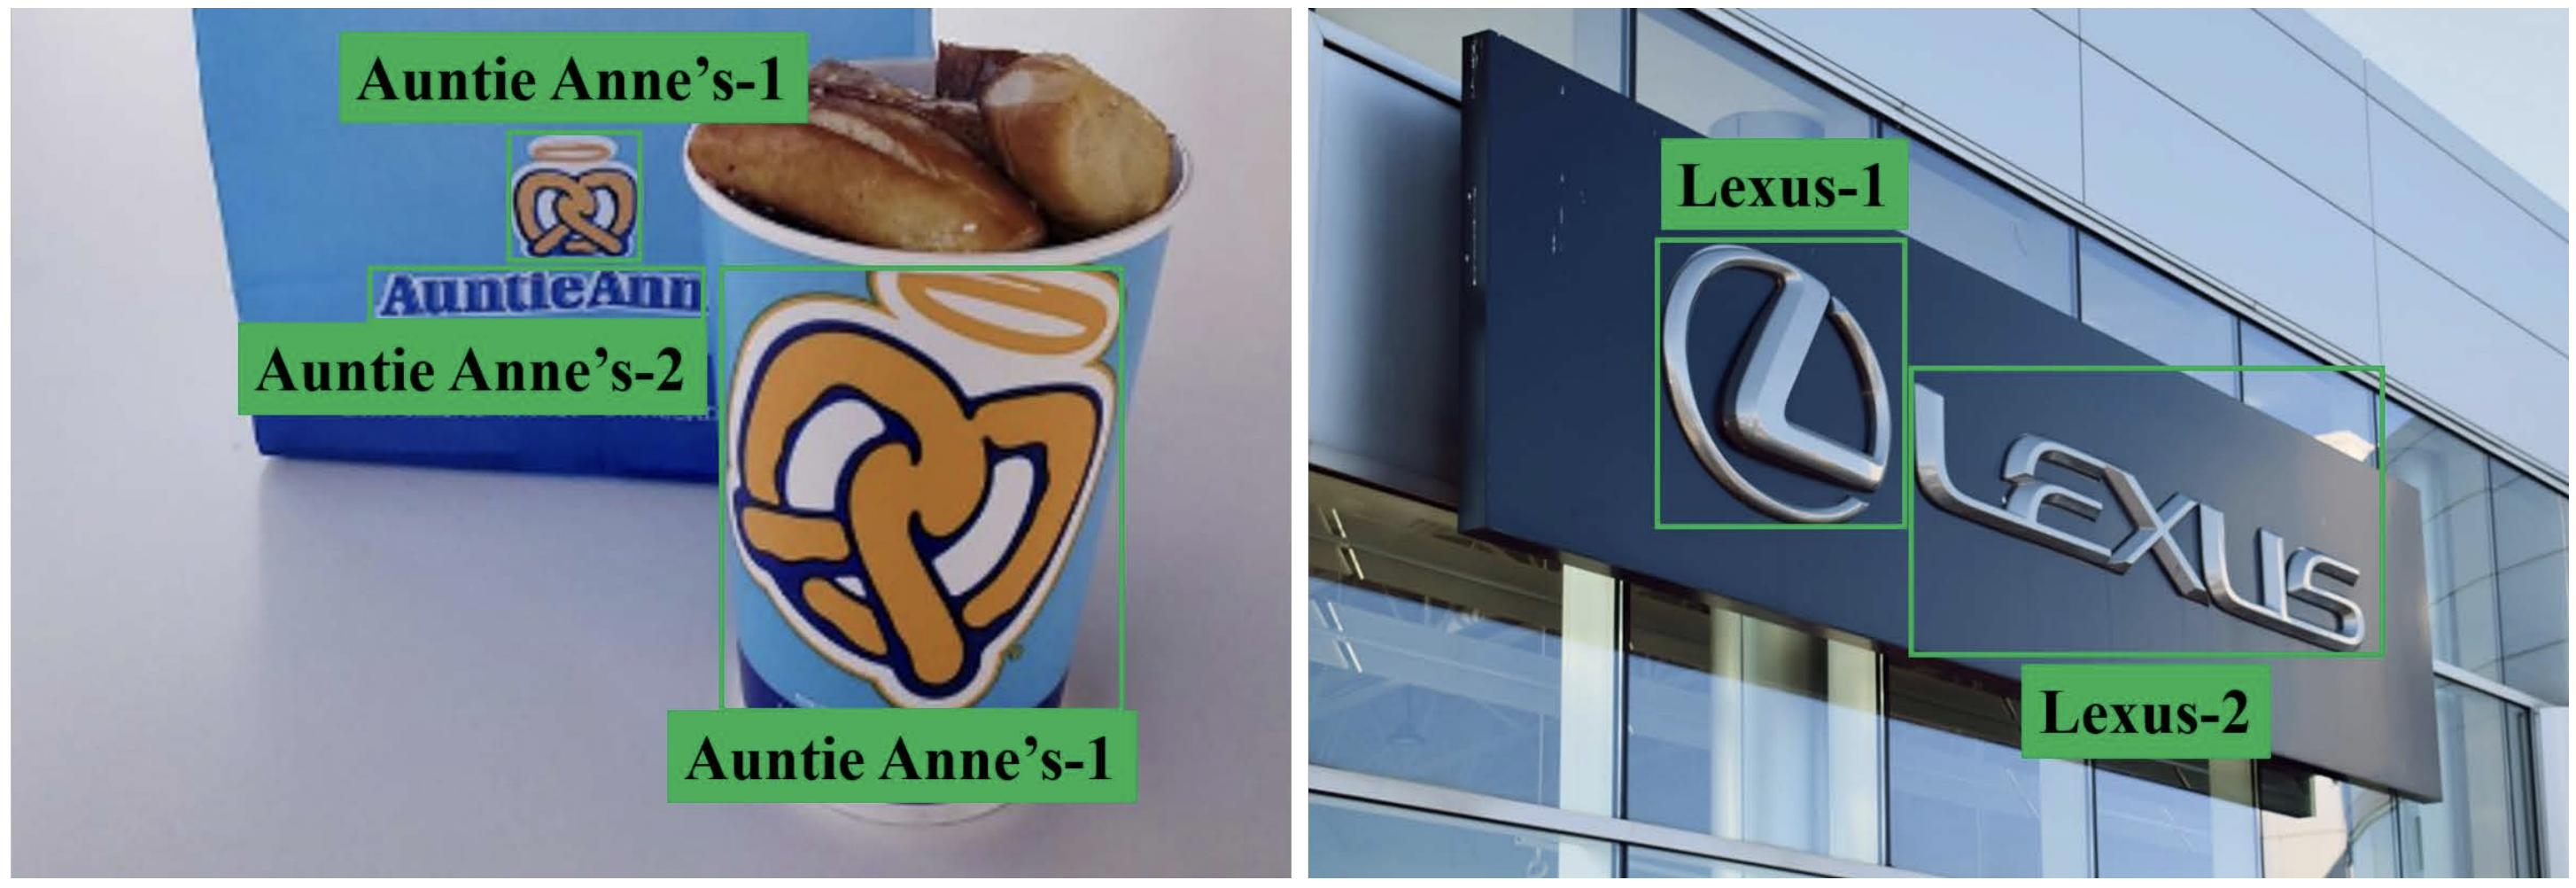
\includegraphics[width=\columnwidth]{images/logos-suffix.png}
    \end{center}
	\caption{Same brand treated as different class using the suffixes '-1' and '-2' \cite{wang2022logodet}.}%
	\label{fig:logos-suffix}%
\end{figure}

\begin{table}
    \centering
    \begin{tabular}{c | c  c  c } 
     \hline
     \textbf{Category} & \textbf{Brand} & \textbf{Images} & \textbf{Objects} \\
     \hline
     Food & 932 & 53,350 & 64,276 \\ 
    Clothes & 604 & 31,266 & 37,601 \\ 
    Necessities & 432 & 24,822 & 30,643 \\ 
    Others & 371 & 15,513 & 20,016 \\ 
    Electronic & 224 & 9,675 & 12,139 \\ 
    Transportation & 213 & 10,445 & 12,791 \\ 
    Leisure & 111 & 5,685 & 6,573 \\ 
    Sports & 66 & 3,953 & 5,041 \\ 
    Medical & 47 & 3,945 & 5,185 \\ 
    \hline
    Total & 3,000 & 158,652 & 194,261 \\ 

    \end{tabular}
    \caption{Brand, images and objects number for each category of LogoDet-3K dataset \cite{wang2022logodet}.}
    \label{table:logodet3k-category-statistics}
\end{table}

\subsection{Dataset statistics}
The \autoref{fig:logodet-dist} shows the distribution of the number of objects for each logo class.

The main issue of LogoDet-3K is the low number of objects for some classes. Analyzing the boxplot in \autoref{fig:logodet-boxplot} and the statistics of \autoref{table:logodet3k-quartile}


\begin{figure}%
	\centering

    \begin{center}
        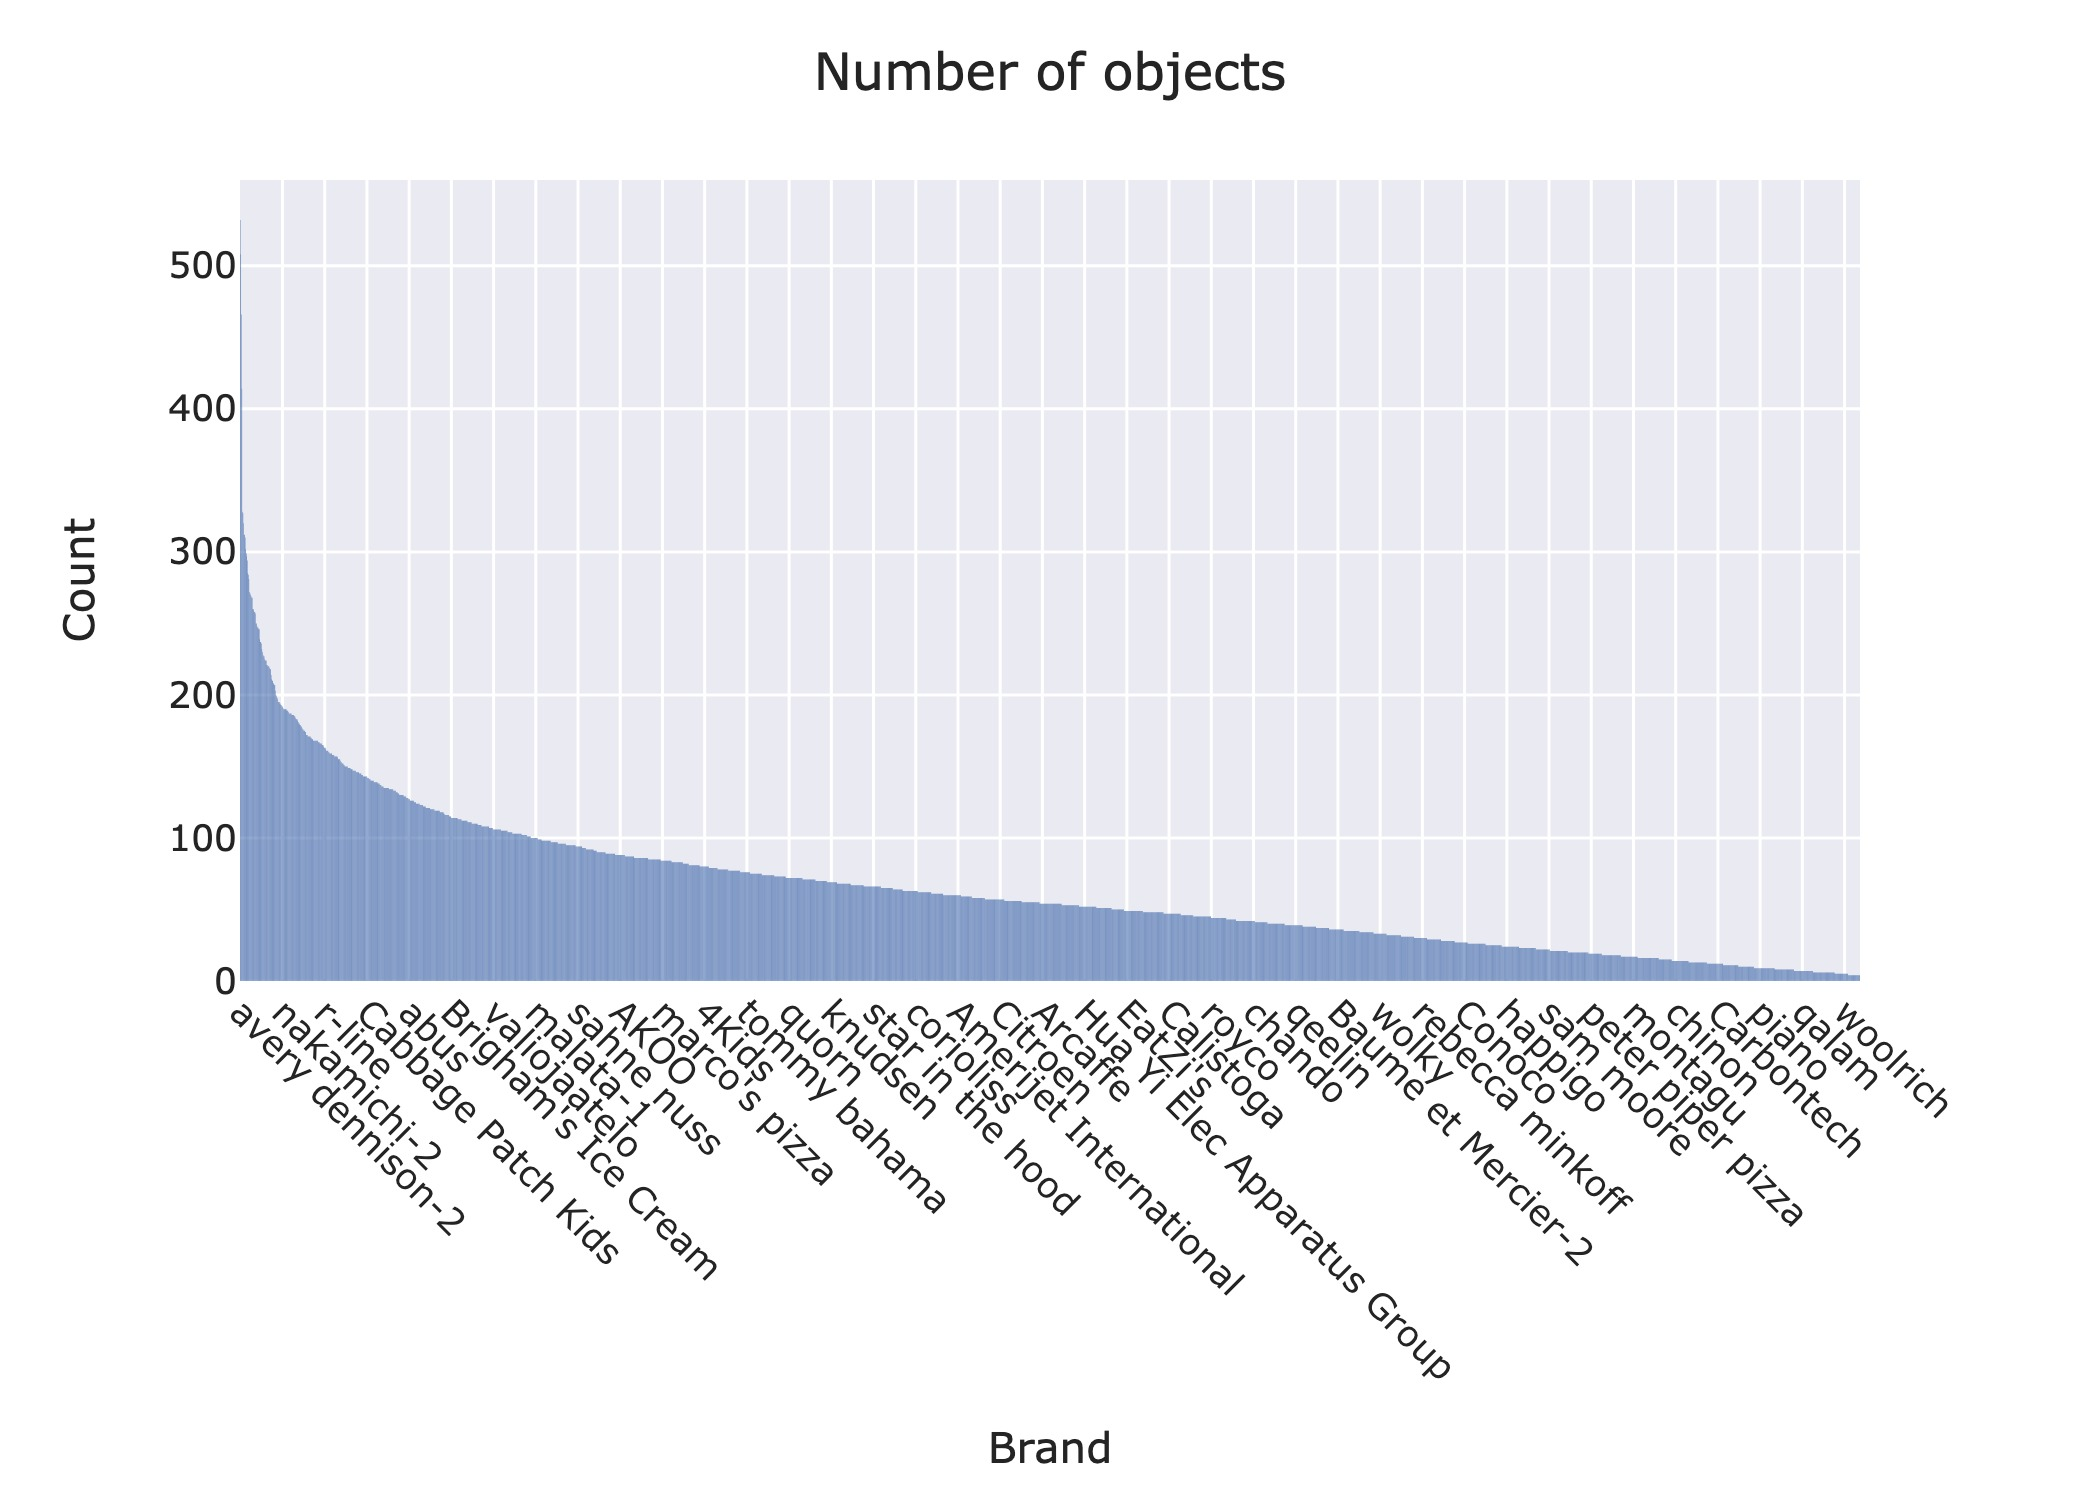
\includegraphics[width=\columnwidth]{images/freq.jpeg}
    \end{center}
	\caption{Number of objects in LogoDet-3K for each class.}%
	\label{fig:logodet-dist}%
\end{figure}


\begin{figure}%
	\centering

    \begin{center}
        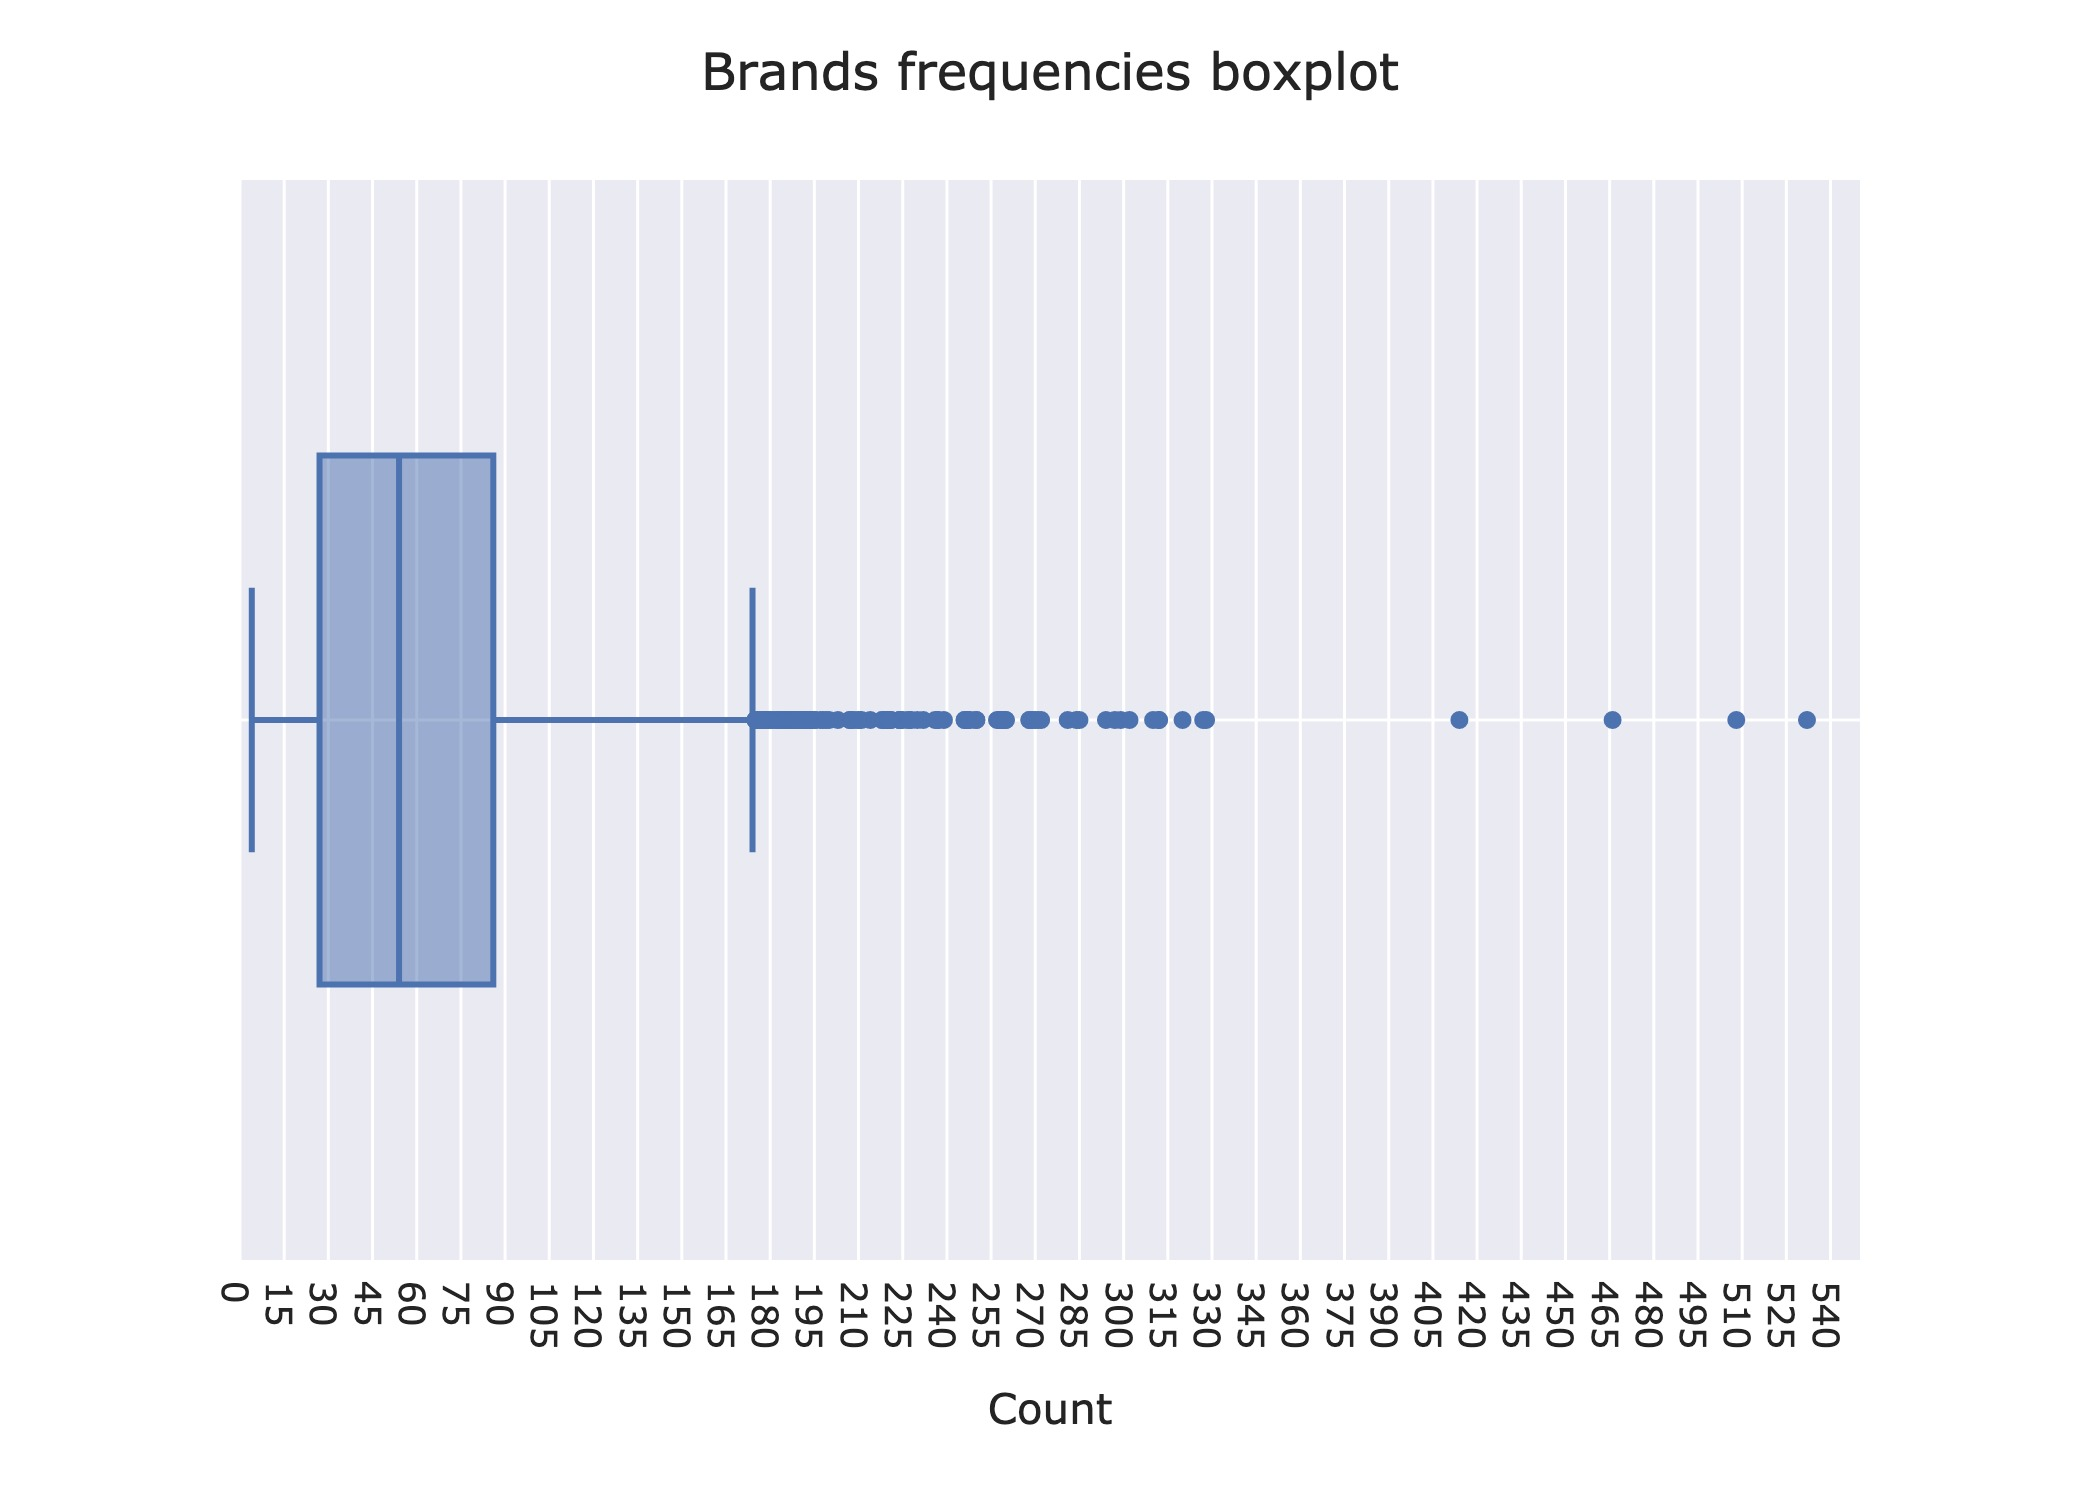
\includegraphics[width=\columnwidth]{images/box_plot.jpeg}
    \end{center}
	\caption{Boxplot of the number of objects in LogoDet-3K for each class.}%
	\label{fig:logodet-boxplot}%
\end{figure}


\begin{table}
    \centering
    \begin{tabular}{c  c  c  c } 
     \hline
     \textbf{$Q_1$} & \textbf{$Q_2$} & \textbf{$Q_3$} & \textbf{$Q_4$} \\
     \hline
     27 & 54 & 86 & 532 \\
    \end{tabular}
    \caption{Quartile relative to the number of objects for each brand in LogoDet-3K dataset.}
    \label{table:logodet3k-quartile}
\end{table}

\section{Inconsistencies in the dataset}


% DA RIMUOVERE - LOREM IPSUM PER DIMOSTRAZIONE
%\foreignlanguage{english}{\Blindtext}

\chapter{Developed methods for logo recognition}
\label{chap:methods}

As discussed in \autoref{chap:introduction}, the system developed in this thesis follows a pipeline consisting of two stages:
\begin{enumerate}
    \item \textbf{Object Proposal}: detection of all the logos in the image
    \item \textbf{Classification}: recognition of the class of each logo
\end{enumerate}
The first stage is done by YOLO (see \autoref{sec:yolo}), while the actual logo recognition is performed by the classifier in an incremental learning setup. The system pipeline is shown in \autoref{fig:roi_and_classification}.

\begin{figure}%
	\centering

    \begin{center}
        \includegraphics[width=\columnwidth]{images/roi+classification.drawio.png}
    \end{center}

	\caption{Pipeline of the system: the class-agnostic logo detector generates Regions of interest (ROIs), then the recognition is performed by the CIL classifier.}%
	\label{fig:roi_and_classification}%
\end{figure}

The detector used in the first stage is a class-agnostic logo detector: it is a logo detector since it only detects logos in the image; and it is class-agnostic since the number of classes detected is only one. In fact, in this first stage the detector will be responsible for finding any generic logo (i.e., a single class) in the image. This is a crucial aspect if we seek to achieve incremental learning logo recognition, because in this way detection can be decoupled from recognition. If the logo detector localizes any generic logo in the image, and delegates the actual recognition to the CIL classifier, there is no need to develop an incremental learning detector as well.

An important aspect of the classifier is the size of the model (in terms of the number of parameters). To this reason, a part of this work aims to decrease the number of parameters of the classifier using two different techniques. The first one is described in \autoref{sec:method-pruning}: using masking and pruning introduced in \autoref{sec:masking-pruning} it aims to prune the model after the training of each incremental step, thus reducing the number of parameters. The second technique is the Knowledge Distillation (KD) described in \autoref{sec:method-kd}, where a smaller model is trained with the supervision of a bigger model trained on the same task.

The code developed in this thesis is available in the GitHub repository\footnote{GitHub repository with the code developed in this thesis: \\ \href{https://github.com/gianlucagiudice/logo-detection-recognition}{https://github.com/gianlucagiudice/logo-detection-recognition}} linked below. The system is developed using the Python programming language, and the code is implemented using PyTorch \cite{paszke2019pytorch}, a widely used deep learning framework. The training of the models is done using the NVIDIA Tesla K80 GPU with 12GB of memory.

\vspace{1.5\baselineskip}
This chapter describes all the details about the logo detector in \autoref{sec:method-roi} and continues with the classifier in \autoref{sec:method-classifier}. Then, in \autoref{sec:method-pruning} and \autoref{sec:method-kd} are discussed some techniques to reduce the number of model parameters. In order to evaluate the drop in performance of the CIL classifier when compared to a standard close-set classification task (i.e. all classes are available from the beginning and no new ones are introduced over time),
the chapter ends in \autoref{sec:method-baseline} with the introduction of different baselines.

\section{Region proposal}
A key component of the system is the logo detector. Formally, this first step is an object detection task, where the objects to be detected are the logos in the image. The logo detector outputs the coordinates of the bounding boxes corresponding to the logos in the image.
Bounding boxes can be used to crop the portions of the image creating regions of interest (ROIs).
ROIs correspond to what the detector considers a generic logo and can be used directly as input to the CIL model that classifies (i.e. recognizes) the logo.

\label{sec:method-roi}
\subsection{YOLOv5m6}
The class-agnostic logo detector is based on YOLOv5-v6.1 \cite{glenn_jocher_2021_5563715}.
There are different versions of YOLOv5-v6.1, depending on the size of the model and the size of the input image.
In general, larger models perform better, with the disadvantage of longer training time, longer inference time and more computational resources required to train the model.
On the other hand, a small model might achieve very low performance, thus misleading the final evaluation of the system that relies heavily on the detector.
Therefore, a model that is too small could act as a bottleneck for the whole system. A more detailed analysis of this trade-off is shown in \autoref{fig:yolo-sizes} and \autoref{table:yolo-sizes}.

\begin{figure}
	\centering

    \begin{center}
        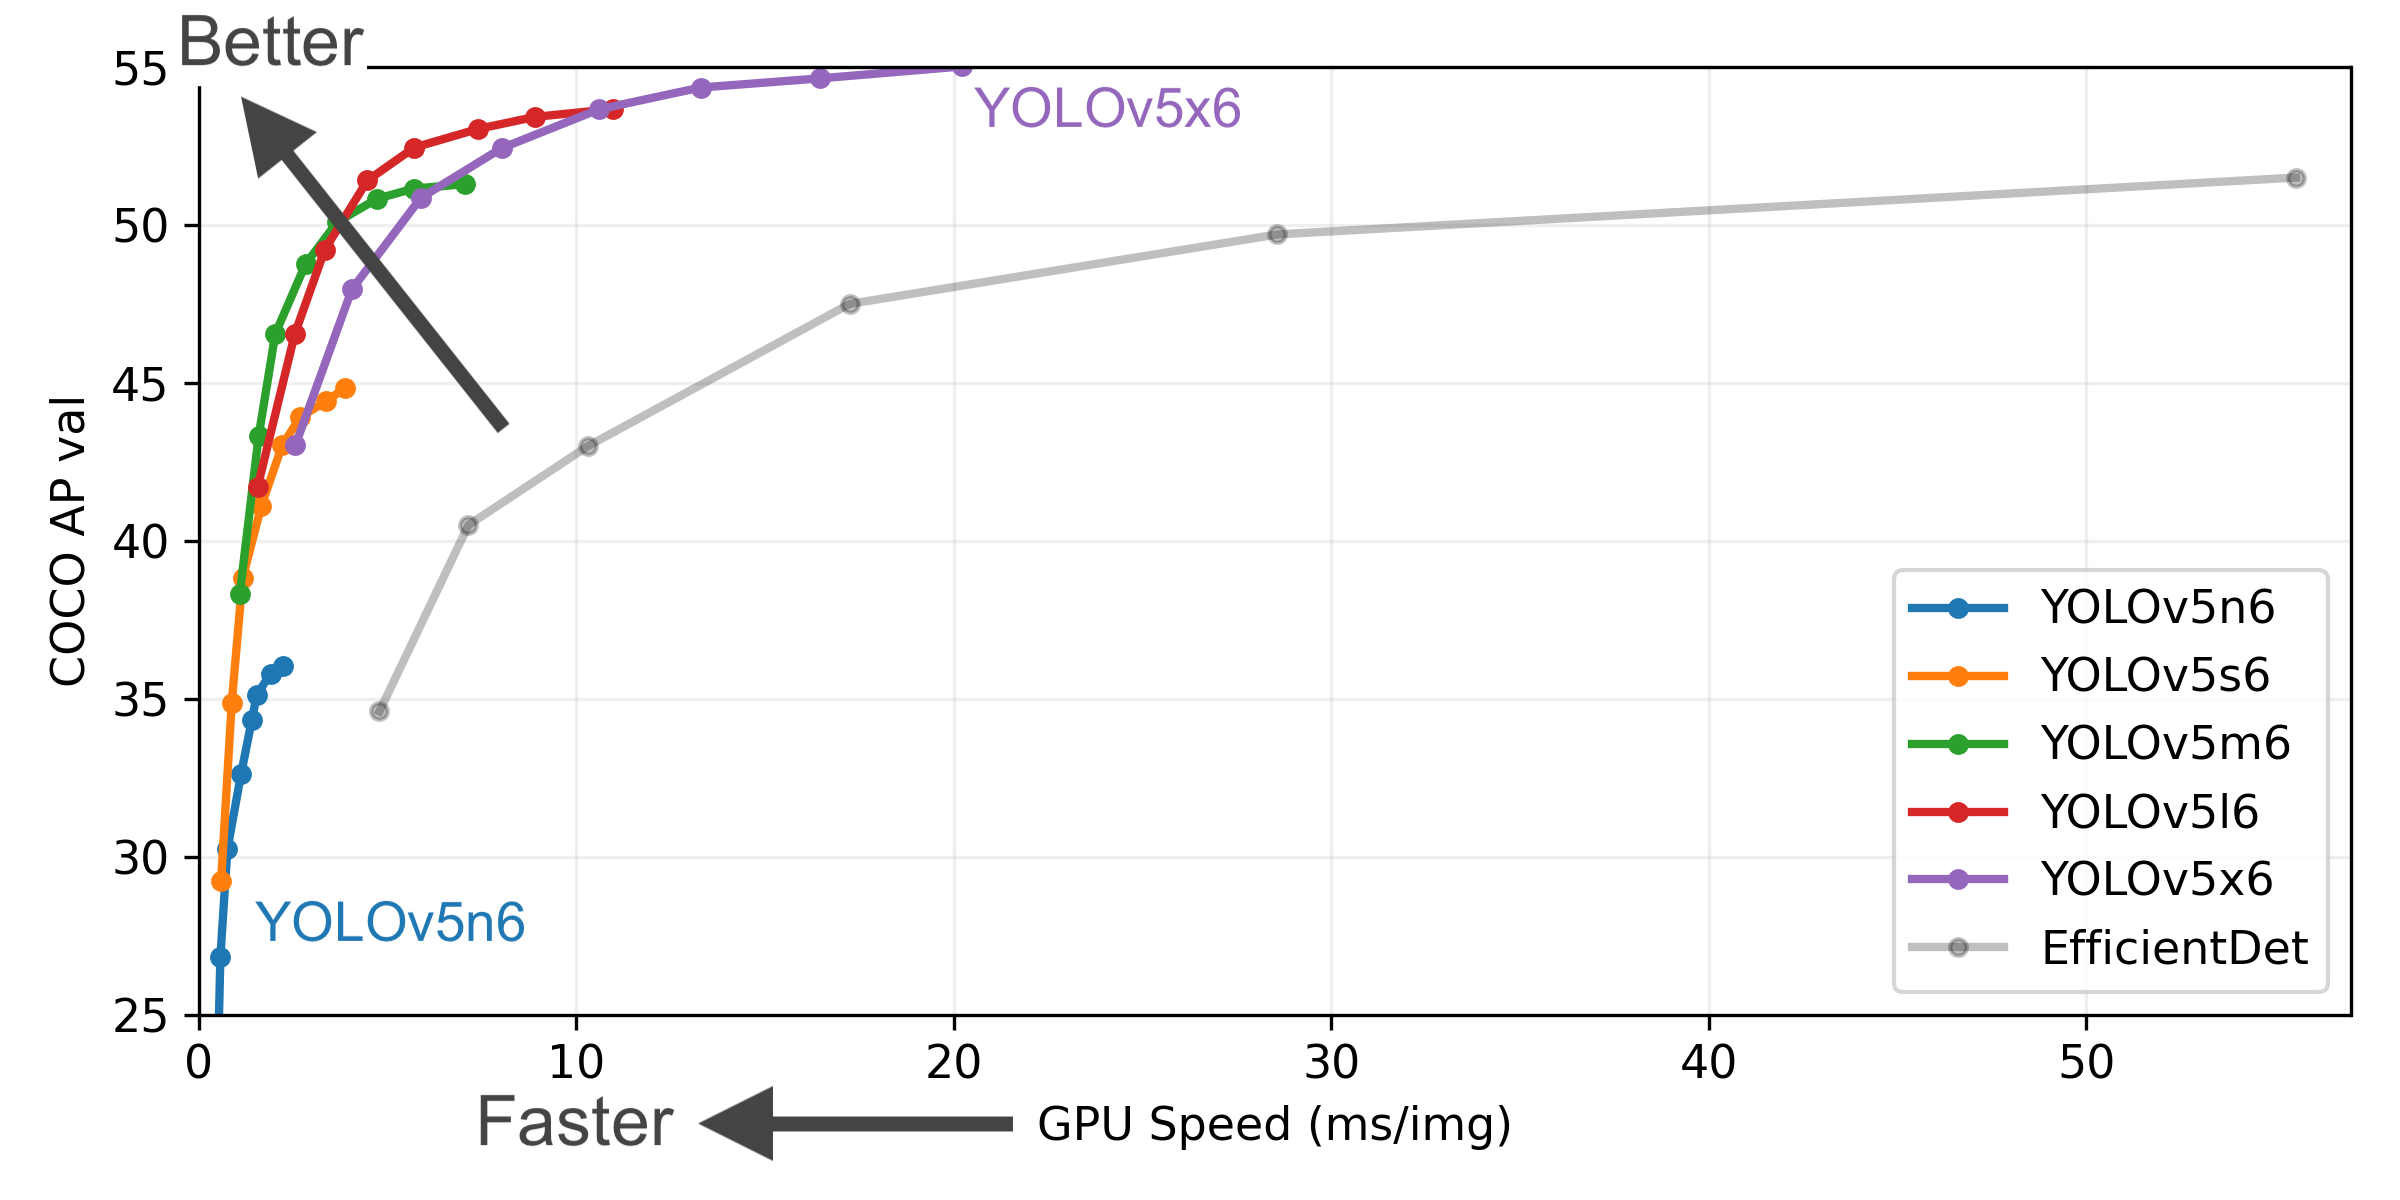
\includegraphics[width=0.9\columnwidth]{images/yolov5-sizes.png}
    \end{center}

	\caption{Performance and speed comparison for the YOLOv5-v6.0 family of models considering the mAP@0.5:0.95 metric measured on the 5000-image COCO val2017 \cite{lin2014microsoft} dataset. The plot shows the performance of different models varying the input size of the image from $256 \times 256$px to $1536 \times 1536$px. Image from \cite{glenn_jocher_2021_5563715}.}
	\label{fig:yolo-sizes}%
\end{figure}


\begin{table}
    \centering
    \centerline{\begin{tabular}{c|c|c|c|c|c|c|c}
        \hline
        \multirow{2}{*}{ \textbf{Model}} & 
        \textbf{size} &
        \textbf{$\text{mAP}^{\text{val}}$} & 
        \textbf{$\text{mAP}^{\text{val}}$} & 
        \textbf{Speed} & 
        \textbf{Speed} & 
        \textbf{\# params} & 
        \textbf{FLOPs} \\
        & (pixels) & \textbf{0.5:0.95} & \textbf{0.5} & \textbf{CPU} (ms) & \textbf{GPU} (ms) & (M) & @640px (B) \\
        \hline
        YOLOv5n & 640 & 28.0 & 45.7 & 45 & 6.3 & 1.9 & 4.5 \\
        YOLOv5s & 640 & 37.4 & 56.8 & 98 & 6.4 & 7.2 & 16.5 \\
        YOLOv5m & 640 & 45.4 & 64.1 & 224 & 8.2 &  21.2 & 49.0 \\
        YOLOv5l & 640 & 49.0 & 67.3 & 430 & 10.1 & 46.5 & 109.1 \\
        YOLOv5x & 640 & 50.7 & 68.9 & 766 & 12.1 & 86.7 & 205.7 \\
        \hline
        YOLOv5n6 & 1280 & 36.0 & 54.4 & 153 & 8.1 & 3.2 & 4.6 \\
        YOLOv5s6 & 1280 & 44.8 & 63.7 & 385 & 8.2 & 12.6 & 16.8 \\
        YOLOv5m6 & 1280 & 51.3 & 69.3 & 887 & 11.1 &  35.7 & 50.0 \\
        YOLOv5l6 & 1280 & 53.7 & 71.3 & 1784 & 15.8 & 76.8 & 111.4 \\
        YOLOv5x6 & 1280 & 55.0 & 72.7 & 3136 & 26.2 & 140.7 & 209.8 \\
        \hline        
        \end{tabular}}
    \caption{Performance comparison considering the mAP@0.5:0.95 metric of all checkpoints of YOLOv5-v6.0 trained for 300 epochs on COCO dataset \cite{glenn_jocher_2021_5563715}.}
    \label{table:yolo-sizes}
\end{table}

The class-agnostic logo detector is based on YOLOv5m6, shown in \autoref{table:yolo-sizes}, with an image input size of $512 \times 512$px and pre-trained on the COCO dataset \cite{glenn_jocher_2021_5563715}.
The model is then finetuned for 30 epochs on the task of class-agnostic logo detection.

\section{Classification}
\label{sec:method-classifier}
Given the ROIs, the classification of each cropped region is performed by a model trained using CIL techniques. To achieve this goal, the classifier is trained using the DER algorithm \cite{yan2021dynamically} described in \autoref{sec:der-algorithm}.

\subsection{ResNet-34}
\label{sec:resnet}
The DER algorithm introduces a new feature extractor $\mathcal{F}_t$ at each incremental step. This feature extractor consists of a CNN. In the developed system the backbone of the CNN is ResNet-34 \cite{he2016deep} pre-trained on ImageNet1000 \cite{deng2009imagenet}.

The peculiar aspects of ResNet architecture are the Residual Connections, shown in \autoref{fig:residual-connection}.
These connections are types of skip-connection that, instead of learning unreferenced functions, learn residual functions with respect to the layer inputs.
Formally, denoting the desired underlying mapping as $\mathcal{H}(x)$, we let the stacked nonlinear layers fit another mapping of $\mathcal{F}(x) := \mathcal{H}(x) - x$. The original mapping is recast into $\mathcal{F}(x) + x$.

The intuition is that it is easier to optimize the residual mapping instead of optimizing the original, unreferenced mapping. In the extreme case, if an identity mapping is optimal, it is easier to push the residual to zero than to fit an identity mapping using a stack of non-linear layers \cite{he2016deep}.

The architecture of ResNet-34, shown in \autoref{table:resnet}, consists of multiple stacked building blocks. Each building block, represented by the brackets in \autoref{table:resnet}, adopts the residual connection described above.
The combination of both skip-connection and batch-normalization (BN) \cite{ioffe2015batch} in ResNet enable the training of a very deep neural network, achieving high performance.
The total number of parameters of ResNet-34 used as feature extractor at each incremental step is 23 million.

\begin{table}
    \centering
    \begingroup
    
    \begin{tabular}{>{\centering\arraybackslash}p{.3\textwidth}|>{\centering\arraybackslash}p{.3\textwidth}|>{\centering\arraybackslash}p{.3\textwidth}}


        \hline
        \multicolumn{3}{c}{\textbf{ResNet-34 architecture}}\\
        \hline
        \textbf{Layer name} & \textbf{Output size} & \textbf{Layer} \\
        \hline
        \hline
        conv1 & $112 \times 122$ & $7 \times 7, 64,$ stride $2$ \\
        \hline
          & $56 \times 56$ & $3 \times 3$ max pool, stride $2$ \\
        \hline

        \[ \textrm{conv2\char`_x} \] &  \[56 \times 56 \] & \[\left[ \begin{array}{c} 3 \times 3, \, 64\\ 3 \times 3, \, 64  \end{array}\right] \times 3 \]\\
        \hline

        \[ \textrm{conv3\char`_x} \] &  \[28 \times 28 \] & \[\left[ \begin{array}{c} 3 \times 3, \, 128\\ 3 \times 3, \, 128  \end{array}\right] \times 4 \]\\
        \hline

        \[ \textrm{conv4\char`_x} \] &  \[14 \times 14 \] & \[\left[ \begin{array}{c} 3 \times 3, \, 256\\ 3 \times 3, \, 256  \end{array}\right] \times 6 \]\\
        \hline

        \[ \textrm{conv5\char`_x} \] &  \[7 \times 7 \] & \[\left[ \begin{array}{c} 3 \times 3, \, 512\\ 3 \times 3, \, 512  \end{array}\right] \times 3 \]\\
        \hline
        & $1000 \times 1$ & average pool \\
        \hline
        FC & $1000 \times 1$ & $1000$-d FC layer, softmax \\
        \hline
        \end{tabular}
    \endgroup
    \caption{Architecture of ResNet-34, the brackets represent a stack of building blocks. }
    \label{table:resnet}
\end{table}

\begin{figure}%
	\centering
	\subfloat[\centering Residual learning: a building block]{{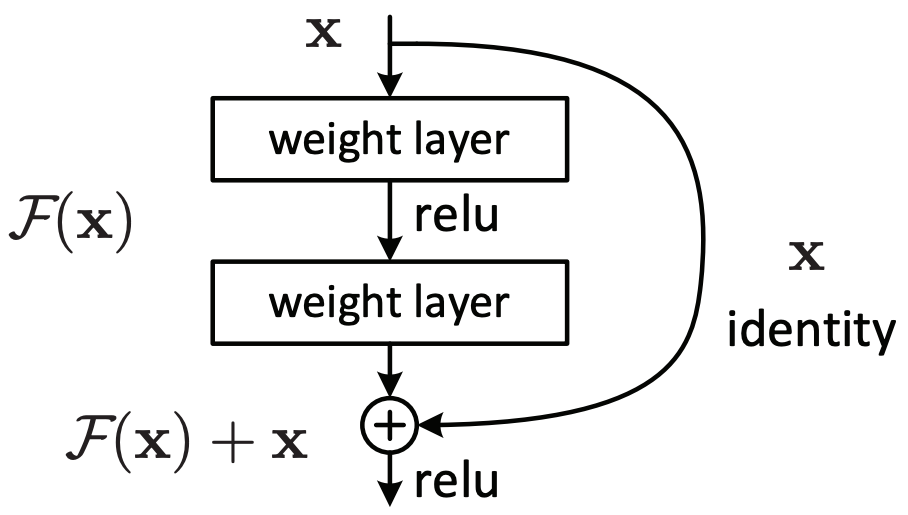
\includegraphics[width=0.45\textwidth]{images/residual-theory.png} }}%
	\hfill
	\subfloat[ An example of residual connection in a building block. This building block corresponds to \textrm{conv2\char`_x} in \autoref{table:resnet} ]{{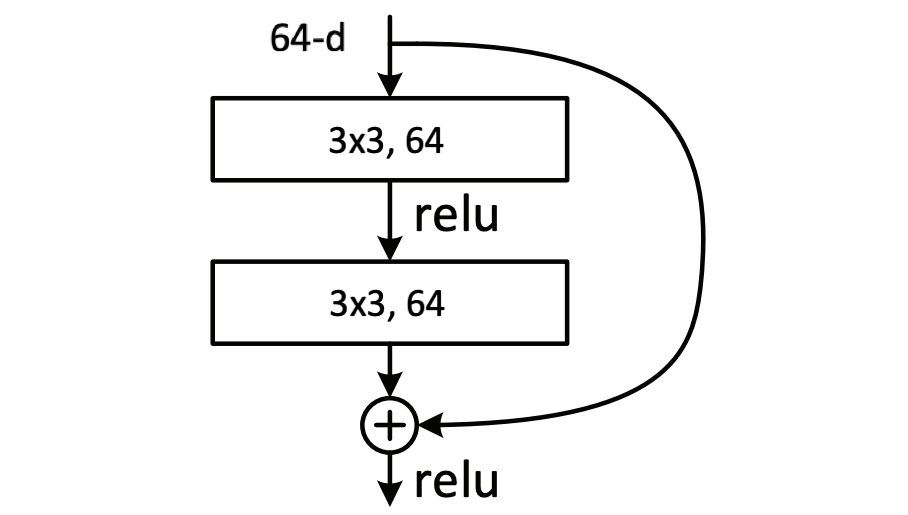
\includegraphics[width=0.45\textwidth]{images/residual-practice.png} }}%
	\caption{Residual connection in ResNet architecture \cite{he2016deep}.}%
	\label{fig:residual-connection}%
\end{figure}

\subsection{CIL classifier}
%The classifier is developed in a CIL setup. This makes it possible to recognise new logos by enriching old knowledge. The algorithm used for CIL is the DER algorithm described in \autoref{sec:der-algorithm}.
An implementation of the DER algorithm is provided by PyCIL\footnote{PyCIL GitHub repository: \\ \href{https://github.com/G-U-N/PyCIL}{https://github.com/G-U-N/PyCIL}} (see \autoref{sec:pycil}), and is used as a starting point for the development of the CIL classifier. 
All the changes made to the implementation of DER in PyCIL are described in the following sections, and can be found in this\footnote{GitHub repository relative to the CIL model of this thesis: \\ \href{https://github.com/gianlucagiudice/PyCIL}{https://github.com/gianlucagiudice/PyCIL}} GitHub repository.

The implementation of DER in PyCIL reflects the description given in the DER paper, with only one difference to the third phase of the DER algorithm (called 'classifier learning phase' in \autoref{sec:der-algorithm}). 
In fact, in PyCIL the 'Classifier Learning Stage' is performed using the WA described in \autoref{sec:wa-biased}; in this way it is possible to solve the problem of biased weights in the FC layer without the need to train the model further.
It is important to emphasize that, although this step of the algorithm is modified, the final performance reported by PyCIL is very similar to that obtained from the original DER implementation (see \autoref{table:cil-results}).

\subsection{Regularization techniques}
To avoid model overfitting, the architecture of the NN created with the DER algorithm is modified.
Starting from the original architecture, a dropout layer is added before the FC layer represented in \autoref{fig:der-pipeline} by the classifier $\mathcal{H}_t$.

\subsubsection{Dropout}
\label{sec:methods-dropout}
DNNs with a large number of parameters are prone to overfitting the training data and do not generalize well on the test set.
Dropout \cite{srivastava2014dropout} is a technique to address this problem.

At training time, the units of the NN, along with their connections, are dropped randomly with a given probability $p$ (a common value is $p = 0.5$). At test time, all units are present, but with weights scaled by $p$ (i.e. $w$ becomes $pw$). This procedure is shown in \autoref{fig:dropout}.

The idea is to prevent co-adaptation, where the NN becomes too reliant on particular connections, as this could be a symptom of overfitting. Intuitively, the dropout can be considered as the creation of an implicit ensemble of NNs.

\begin{figure}%
	\centering
	\subfloat[\centering Standard neural network]{{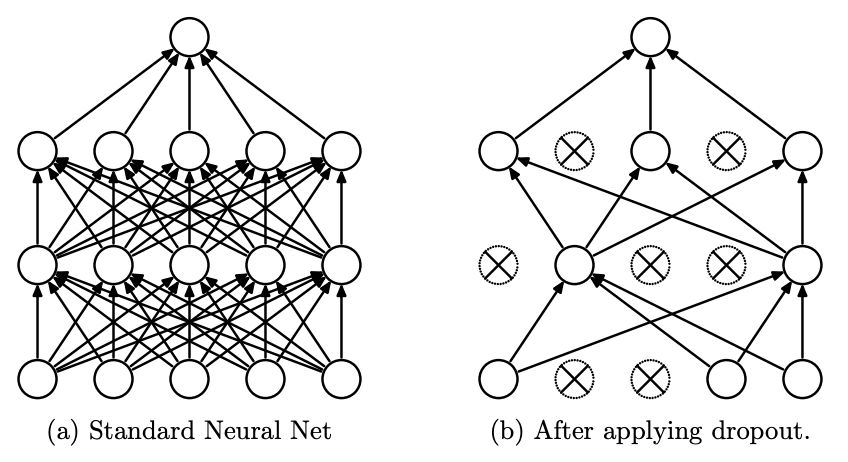
\includegraphics[width=0.30\textwidth,trim={0 24 220 0},clip]{images/dropout.png} }}%
	\hspace*{2cm}
	\subfloat[\centering Neural network after applying dropout ]{{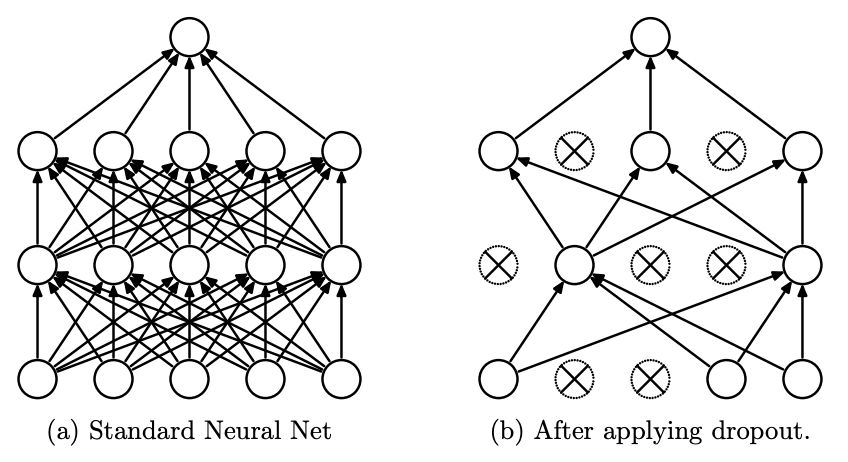
\includegraphics[width=0.30\textwidth,trim={220 24 0 0},clip]{images/dropout.png} }}%
	\caption{Dropout mechanism in a Neural Network with 2 hidden layers \cite{srivastava2014dropout}.}%
	\label{fig:dropout}%
\end{figure}

\subsection{Data augmentation}
\label{sec:methods-augment}
As discussed in \autoref{sec:dataset-stat}, one problem with the LogoDet-3K dataset is that some classes have a low number of images. Moreover, as shown in \autoref{table:logodet3k-quartile}, these classes are not an exception but the majority of those in the dataset. In fact, 50\% of the dataset has a number of images less than or equal to 54.

Training a model using a small number of examples per class can be a problem in machine learning in general, but this is particularly true in the deep learning domain, where models require a huge amount of data.

Image augmentation is a data augmentation method that generates more training data from the existing training samples.
This is a very useful technique to address the problem of low number of images per class in LogoDet-3K.
In addition, data augmentation is another way to avoid overfitting, as it creates synthetic samples by adding random perturbations to the original image, yet preserving its main characteristics, thus achieving better generalization.

The type of data augmentation adopted during the training of the model is called online data augmentation.
This technique consists in applying a random transformation to the original image before feeding it to the model.
In this way, it is theoretically possible to obtain an infinitely large dataset. The process of data augmentation is heavily dependent on the type of transformations applied to the images: an excessive transformation of the original image may mislead the model in learning the main features of the image, while keeping the image as similar as possible to the original one may have the same effect as not applying data augmentation at all.

The transformations used to augment the original dataset, shown in \autoref{fig:example-augmentation}, and used to train the CIL classifier are the following:
\begin{itemize}
    \item \textbf{Geometric transformations}:
    \begin{itemize}
        \item \textbf{Random affine}: transforms the image while keeping the centre invariant.
        \item \textbf{Random perspective}: perspective transformation of the image.
    \end{itemize}
    \item \textbf{Color transformations}:
    \begin{itemize}
        \item \textbf{Adjust sharpness}: transforms the original image into a sharper one according to the sharpening factor. This parameter is chosen a priori and is fixed for each transformation.
        \item \textbf{Posterize}: reduces the number of bits for each color channel.
        \item \textbf{Color jitter}: randomly changes the brightness, contrast, saturation and hue of an image.
    \end{itemize}
\end{itemize}

As previously stated, the data augmentation is performed in an online manner, in this way it is possible to obtain a slightly different image at each training epoch of the model.
The original image is transformed using the transformations listed above, but the final image is a combination of geometric and color transformations. 
This procedure is shown in \autoref{fig:data_augmentation}, and is applied to different logos in \autoref{fig:final_data_augmentation}.

\begin{figure}[H]
	\centering

    \begin{center}
        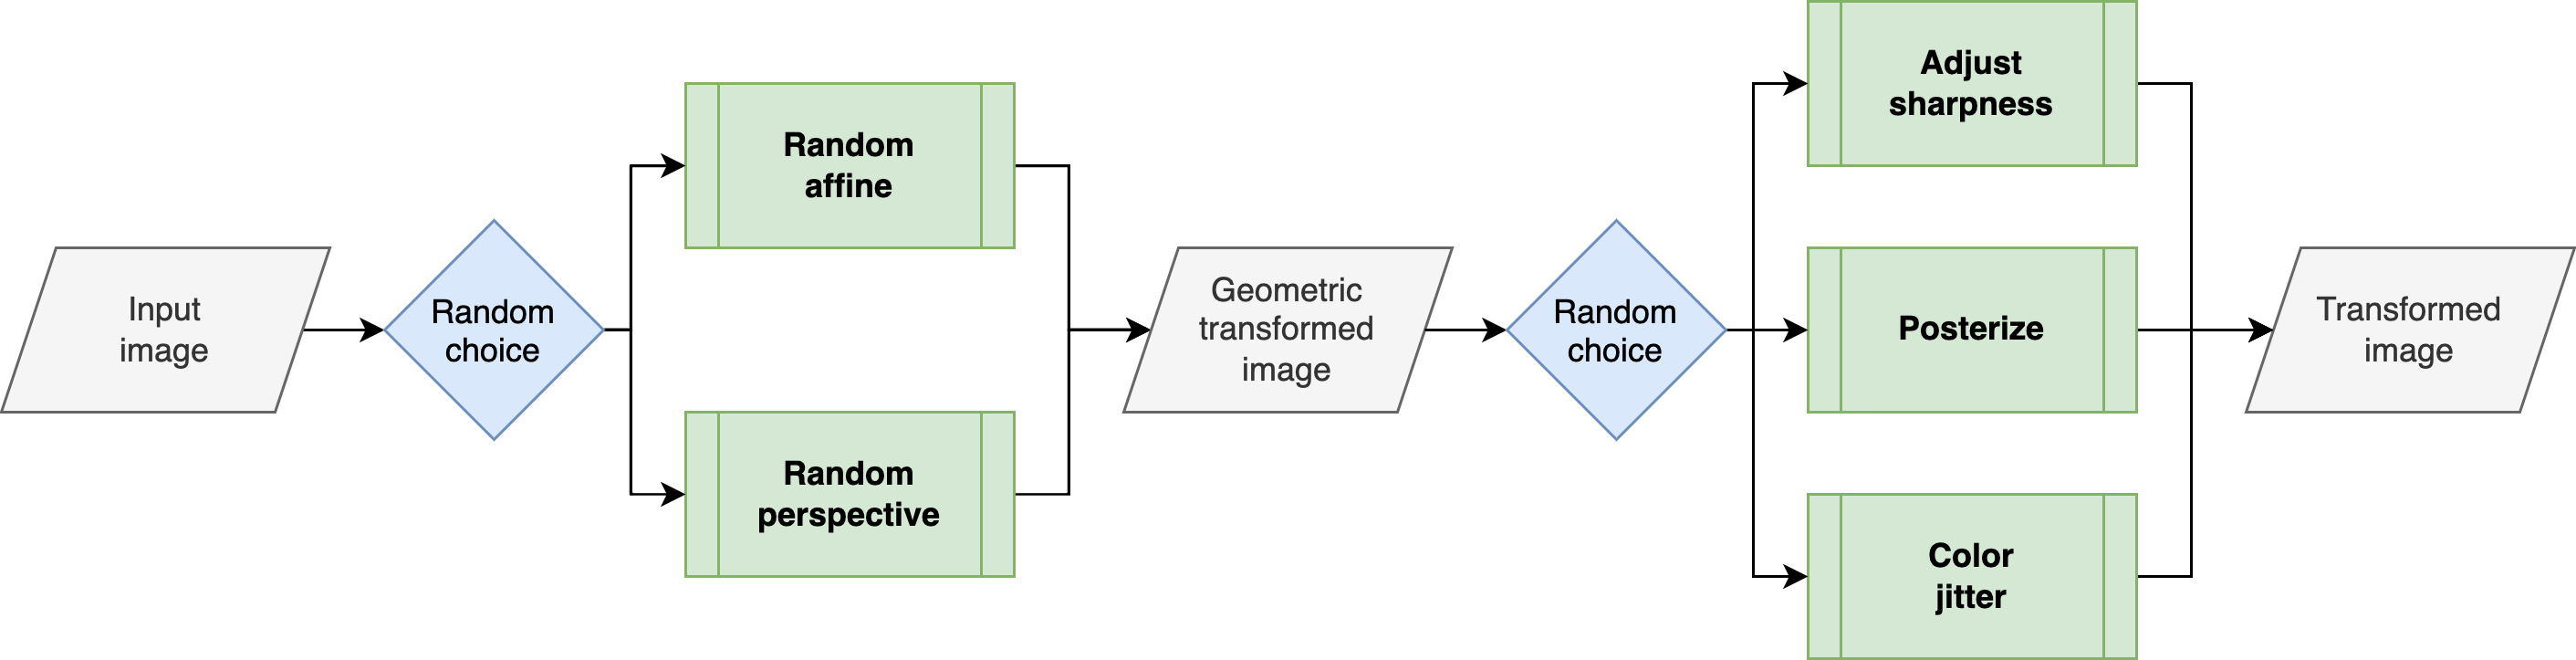
\includegraphics[width=\columnwidth]{images/data_augmentation.drawio.png}
    \end{center}

	\caption{Image transformation pipeline for data augmentation: first the input image is transformed via a geometric transformation, then a color transformation is applied.}%
	\label{fig:data_augmentation}%
\end{figure}

\newpage

\begin{figure}[H]
    \centering
    \subfloat[Original image]{{
\includegraphics[height=3cm]{images/augmentations/original.jpg} }}%
    \hfill
    \subfloat[Random affine transformation]{{
\includegraphics[height=3cm]{images/augmentations/affine.jpg} }}%
    \hfill
    \subfloat[Random perspective transformation]{{
\includegraphics[height=3cm]{images/augmentations/perspective.jpg} }}%
    \hfill
    \subfloat[Adjust sharpness]{{
\includegraphics[height=3cm]{images/augmentations/sharpness.jpg} }}%
    \hspace*   {2cm}
    \subfloat[Posterize]{{
\includegraphics[height=3cm]{images/augmentations/posterize.jpg} }}%
    \hfill
    \subfloat[Random color Jitter]{{
\includegraphics[height=3cm]{images/augmentations/color_jitter.jpg} }}%
    \caption{Examples of image transformations. The transformations (d) and (e) are shown in a single image since, given the sharpness factor and the number of bin for the posterization, the result of the transformation is always the same.}%
    \label{fig:example-augmentation}%
\end{figure}

\begin{figure}[H]
	\centering
	\subfloat[Logo 1]{{
\includegraphics[height=2cm]{images/augmentations/transf1.png} }}%
	\hfill
	\subfloat[Logo 2]{{
\includegraphics[height=2cm]{images/augmentations/transf2.png} }}%
	\hfill
	\subfloat[Logo 3]{{
\includegraphics[height=2cm]{images/augmentations/transf3.png} }}%
	\hfill
	\subfloat[Logo 4]{{
\includegraphics[height=2cm]{images/augmentations/transf4.png} }}%
	\hfill
    \subfloat[Logo 5]{{
\includegraphics[height=2cm]{images/augmentations/transf5.png} }}%
	\hfill
    \subfloat[Logo 6]{{
\includegraphics[height=2cm]{images/augmentations/transf6.png} }}%
	\caption{Examples of data augmentation on different logos: the first column represents the original image, the other columns are some transformation applied to the original image following the pipeline described in \autoref{fig:data_augmentation}.}%
	\label{fig:final_data_augmentation}%
\end{figure}

\subsection{Training}
The training of the CIL model can be divided into two main steps: the initial task and the iterations of CIL. At the initial task the model is trained for 200 epochs, while for the incremental learning iterations it is trained for 150 epochs.

The number of training epochs at the initial task is higher because in this phase the network requires a longer time to converge, this is due to these two factors: the neural network must adapt the weights trained on ImageNet to the logo classification task; it is assumed that the number of classes at the initial task is greater than the number of classes introduced at each incremental learning iteration.

\subsubsection{Early stopping}
Early stopping is used to avoid overfitting of the model.
This is done by monitoring the accuracy of the model during training on the validation set.
The hyperparameters of early stopping are the following: the number of epochs with no improvement after which training will be stopped is set to 30 (i.e. patience); the minimum change in the monitored accuracy to be considered as an improvement is set to 0.5\% (i.e., the minimum delta).

\subsubsection{SGD optimizer}
\label{sec:sgd_opt}
To update the model weights two different optimizers are tested.
One of them is Stochastic Gradient Descent (SGD), an iterative method for optimizing an objective function.

As described in \cite{zhang2021dive}, in deep learning the objective function is usually the average of the loss functions for each example in the training dataset. Given a training dataset of $n$ examples, we assume that $f_i(\textbf{w})$ is the loss function with respect to the training example of index $i$, where $\textbf{w}$ is the parameter vector. Then the objective function is given by:
\begin{equation}
    f(\textbf{w}) = \frac{1}{n} \sum_{i=1}^n f_i(\textbf{w})
\end{equation}
The gradient of the objective function at $\textbf{w}$ is computed as:
\begin{equation}
    \nabla f(\textbf{w}) = \frac{1}{n} \sum_{i=1}^n \nabla f_i(\textbf{w})
\end{equation}
Using gradient descent, the computational cost for each independent iteration is $\mathcal{O}(n)$, which grows linearly with $n$. Therefore, when the training dataset is larger, the cost of gradient descent for each iteration will be higher.

SGD reduces the computational cost at each iteration by uniformly sampling an index $i \in \{ 1, \, ..., \, n\}$ from data examples, and computes the gradient $\nabla f_i (\textbf{w})$ to update $\textbf{w}$ as follows:

\begin{equation}
    \textbf{w} \leftarrow \textbf{w} - \eta \nabla f_i(\textbf{w})
\end{equation}
where $\eta$ is the learning rate ($\eta = 0.1$ in the experiments described in \autoref{chap:experiments}). In this way the computational cost for each iteration drops from $\mathcal{O}(n)$ of the gradient descent to the constant $\mathcal{O}(1)$ of SGD. Moreover, the stochastic gradient $\nabla f_i(\textbf{w})$ is an unbiased estimate of the full gradient $\nabla f(\textbf{w})$, since:
\begin{equation}
    \mathbb{E}_i \nabla f_i(\mathbf{w}) = \frac{1}{n} \sum_{i = 1}^n \nabla f_i(\mathbf{w}) = \nabla f(\mathbf{w})
\end{equation}
This means that, on average, the stochastic gradient is a good estimate of the gradient.

A compromise between computing the true gradient and the gradient with a single sample is to compute the gradient against more than one training sample (called a 'mini-batch'). This means replacing the gradient $\nabla f_i(\textbf{w})$ on a single observation with one over a small batch $\mathcal{B}_t = \{ \textbf{x}^{(1)},\, ..., \, \textbf{x}^{(m)}\}$ (for the experiments described in \autoref{chap:experiments}, $|\mathcal{B}_t| = 2048$). Then, the gradient $\textbf{g}_t$ over a small batch $\mathcal{B}_t$ is given by:
\begin{equation}
    \mathbf{g}_t = \frac{1}{|\mathcal{B}_t|} \sum_{i \in \mathcal{B}_t} \nabla f_i(\mathbf{w})
\end{equation}
Note that, during an epoch, the examples are not reused for multiple batches. The minibatch SGD algorithm is shown in \autoref{alg:sgd}, as described by Goodfellow et al. in \cite{Goodfellow-et-al-2016}.


\begin{algorithm}
    \caption{SGD algorithm with minibatches}\label{alg:sgd}
    \begin{algorithmic}
        \Require Learning rate $\eta$
        \Require Initial parameters $\textbf{w}$
        
    \While{stopping criterion not met}
        
        Sample a minibatch $\mathcal{B}$ of $m$ examples from the training set $\{ \textbf{x}^{(1)},\, ..., \, \textbf{x}^{(m)}\}$ with corresponding labels $\textbf{y}^{(i)}$.

    Compute gradient estimate: $\hat{\mathbf{g}} = \frac{1}{|\mathcal{B}|} \sum_{i \in \mathcal{B}_t} \nabla f_i(\mathbf{w})$.

    Apply update: $\textbf{w} \leftarrow \textbf{w} - \eta \hat{\mathbf{g}}$.

    \EndWhile
    \end{algorithmic}
    \end{algorithm}


\subsubsection{Adam optimizer}
\label{sec:adam_opt}
The second optimizer used in the experiments is Adam \cite{kingma2014adam}, which can be considered as a combination of RMSProp \cite{hinton2012neural} and momentum \cite{sutskever2013importance}. Adam is an adaptive learning rate optimizer, i.e. it uses a separate learning rate for each parameter and automatically adapts these learning rates throughout the course of learning. A key component of Adam is that it uses exponential weighted moving averages (also known as leaky averaging) to obtain an estimate of the momentum of the gradient.

To estimate the first-order and the second-order moments of the gradient, Adam uses two state variables:
\begin{equation}
    \begin{split}\begin{aligned}
        \mathbf{v}_t & \leftarrow \beta_1 \mathbf{v}_{t-1} + (1 - \beta_1) \mathbf{g}_t \\
        \mathbf{s}_t & \leftarrow \beta_2 \mathbf{s}_{t-1} + (1 - \beta_2) \mathbf{g}_t^2
    \end{aligned}\end{split}
\end{equation}
where $\beta_1$ and $\beta_2$ are nonnegative weighting parameters. In the experiments in \autoref{chap:experiments}, $\beta_1=0.9$ and $\beta_2=0.999$.

Initially, both $\mathbf{v}_0$ and $\mathbf{s}_0$ are set to 0, resulting in a bias towards smaller values. For this reason, Adam computes the bias-corrected $\hat{\mathbf{v}}_t$ and $\hat{\mathbf{s}}_t$ as follows:
\begin{equation}
    \begin{split}\begin{aligned}
        \hat{\mathbf{v}}_t & = \frac{\mathbf{v}_t}{1 - \beta_1^t} \\
        \hat{\mathbf{s}}_t & = \frac{\mathbf{s}_t}{1 - \beta_2^t}
    \end{aligned}\end{split}
\end{equation}
Then, the gradient is rescaled accordingly to consider both the first-order and second-order moments:
\begin{equation}
    \mathbf{g}_t' = \eta \frac{ \hat{\mathbf{v}}_t}{\sqrt{\hat{\mathbf{s}}_t} + \epsilon}
\end{equation}
where, $\eta$ is the learning rate (set to $0.001$ in the experiments in \autoref{chap:experiments}) and $\epsilon = 10^{-8}$ is a constant to achieve numerical stability.

Finally, the parameters are updated as follows:
\begin{equation}
    \textbf{w}_t \leftarrow \textbf{w}_{t-1} - \mathbf{g}_t'
\end{equation}

The Adam algorithm is shown in \autoref{alg:adam}, as described by Goodfellow et al. in \cite{Goodfellow-et-al-2016}.

\begin{algorithm}
    \caption{The Adam algorithm}\label{alg:adam}
    \begin{algorithmic}
        \Require Learning rate $\eta$
        \Require Exponential decay rates for moment estimates, $\beta_1$ and $\beta_2$ in $[0, \, 1)$ (Suggested defaults: $0.9$ and $0.999$ respectively).
        \Require Small constant $\epsilon$ used for numerical stabilization (Suggested default: $10^{-8}$).
        \Require Initial parameters $\textbf{w}$\\
        Initialize 1st and 2nd moment variable $\mathbf{s} = 0$, $\mathbf{r} = 0$\\
        Initialize time step $t = 0$
    \While{stopping criterion not met}
        
        Sample a minibatch $\mathcal{B}$ of $m$ examples from the training set $\{ \textbf{x}^{(1)},\, ..., \, \textbf{x}^{(m)}\}$ with corresponding labels $\textbf{y}^{(i)}$.
        
        Compute gradient estimate: $\hat{\mathbf{g}} = \frac{1}{|\mathcal{B}|} \sum_{i \in \mathcal{B}_t} \nabla f_i(\mathbf{w})$.

        $t \leftarrow t +1$
        
        Update biased first moment estimate: $\mathbf{v} \leftarrow \beta_1 \mathbf{v} + (1 - \beta_1) \mathbf{\hat{g}}$

        Update biased second moment estimate: $\mathbf{s} \leftarrow \beta_2 \mathbf{s} + (1 - \beta_2) \mathbf{\hat{g}}^2$

        Correct bias in first moment: $\hat{\mathbf{v}} = \frac{\mathbf{v}}{1 - \beta_1^t}$
  
        Correct bias in second moment: $\hat{\mathbf{s}} = \frac{\mathbf{s}}{1 - \beta_2^t}$

        Compute update: $\Delta \mathbf{w} = \eta \frac{ \hat{\mathbf{v}}}{\sqrt{\hat{\mathbf{s}}} + \epsilon}$

        Apply update: $\textbf{w} \leftarrow \textbf{w} - \Delta \mathbf{w}$.

    \EndWhile
    \end{algorithmic}
    \end{algorithm}

\subsubsection{Learning rate decay}
For both SGD and Adam, an exponential decay scheduling is applied to the learning rate: once one epoch reaches one of the predetermined epochs (called milestones) the learning rate of the optimizer is multiplied by a factor $\gamma = 0.1$. For the training of the CIL classifier, the milestones are set to 60, 100 and 150 for the initial task, and to 40, 75 and 100 for each incremental learning iteration.

Adjusting the learning rate is an important aspect of the optimization process. Some of the motivations behind learning rate scheduling are described below:
\begin{itemize}
    \item The magnitude of the learning rate is a key factor in the optimization procedure: if the learning rate is too large, optimization diverges, while if it is too small, either training takes too long or a suboptimal result is achieved.
    \item If the learning rate remains high, the algorithm may bounce around the minimum or even jump over it and thus failing to reach optimality. 
\end{itemize}

The learning rate decay is used to train models for the experiments described in \autoref{chap:experiments}. An example of the effect of the learning rate decay is shown in \autoref{fig:lr_decay}.
By plotting the accuracy of the model at each training epoch, it is possible to notice that, when a milestone is reached (epoch 60) and the learning rate is scaled by a factor of $10^{-1}$, there is an improvement in the accuracy of the model in subsequent epochs.

\begin{figure}[H]
	\centering

    \begin{center}
        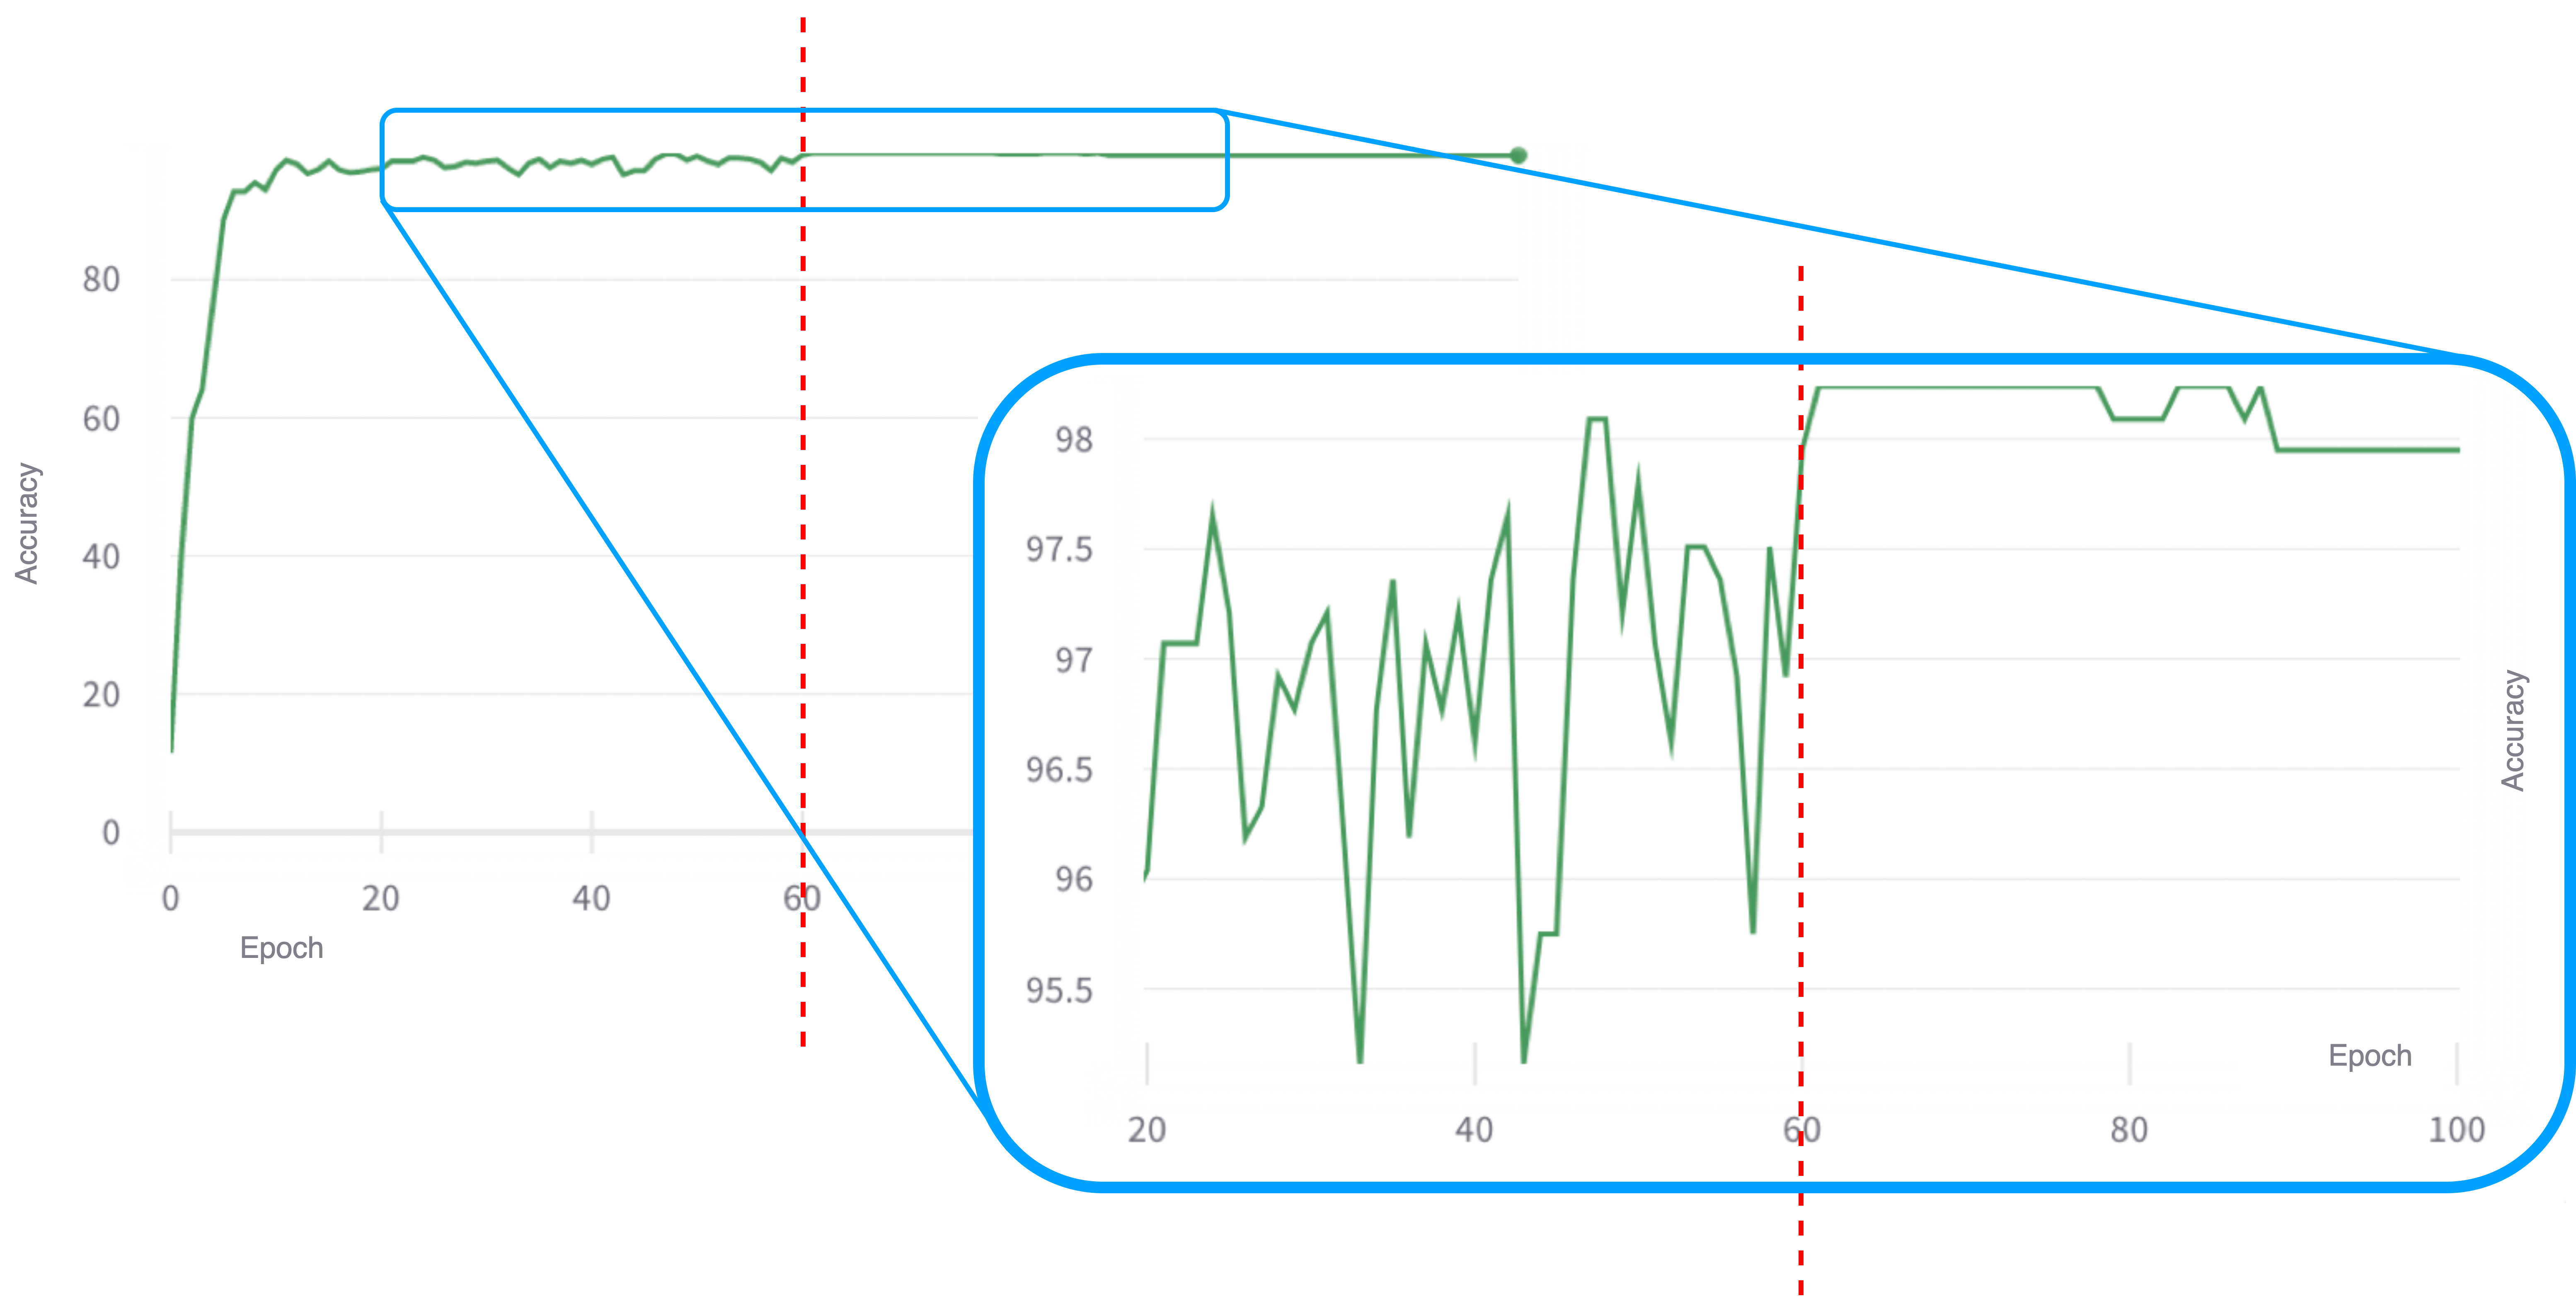
\includegraphics[width=\columnwidth]{images/lr_decay.drawio.png}
    \end{center}

	\caption{Effect of the learning rate decay: the figure shows the accuracy of the model at each training epoch. At epoch 60, the learning rate is scaled by a factor of $10^{-1}$, this leads to an increase in the model's accuracy in subsequent epochs.}
	\label{fig:lr_decay}%
\end{figure}


\subsection{Pruning}
\label{sec:method-pruning}

The DER algorithm, described in \autoref{sec:der-algorithm}, addresses the problem of class incremental learning by expanding the neural network architecture at each incremental step. The super-feature extractor at step $t$ of incremental learning is given by the following concatenation $\Phi_t(\mathbf{x}) = [\mathcal{F}_0, \, \mathcal{F}_1(\mathbf{x}), \, ..., \, \mathcal{F}_t(\mathbf{x})]$. As discussed in \autoref{sec:resnet}, the feature extractor is a CNN, which in this thesis is implemented using ResNet-34.

Given the definition of the super-feature extractor, it is possible to see how the parameters of the neural network grow linearly as a function of the number of incremental learning steps.
It is important to note that as the parameters of the super-feature extractor increase, those of the classifier $\mathcal{H}_t$ do as well.
The classifier $\mathcal{H}_t$ corresponds to the fully connected layer of the neural network. At each incremental learning task new classes are introduced, thus new connections are created between the classifier predicting the output class and the super-feature extractor.

This means that, using the LogoDet-3K dataset described in \autoref{chap:dataset}, and the incremental learning setup described in \autoref{sec:whole_dataset_clf}, at the 8th step of CIL the total number of parameters is given by: the number of parameters at task 0 (initial task), in which 22 million parameters (number of parameters of ResNet-34) are used; the 8 incremental learning steps, each adding 22 million parameters to the total.

After only 8 iterations of incremental learning, the final neural network reaches 205 million parameters, which is a large number of parameters compared to a single ResNet-34 used as backbone of each feature extractor.
For this reason, there is a need to reduce the number of parameters of the neural network.
To do so, the pruning of the network is implemented using masks, as described in \autoref{sec:masking-pruning}.

Each mask $\mathbf{m}_l$ associated with the channels of each layer $l$ of the CNN is computed as shown in \autoref{eq:mask}.
At the incremental learning task $t$, after the training of the feature extractor $\mathcal{F}_t(\mathbf{x})$, the variable $s$ is set to a really high value ($10^{4}$ in the implementation).
Since $s$ is fed into the sigmoid used as gating function, a steep activation mechanism is obtained (which leads to a binary activation when the limit of $s$ tends to infinity, but this behavior is achieved in practice using high value of $s$).
So, if a value $e_{li}$ of the mask $\mathbf{e}_l$ is positive, $m_{li}$ tends to 1, else if $e_{li}$ is negative, $m_{li}$ tends to 0.
To perform the actual binarization of each mask value, a threshold $\tau$ with a low value set to $10^{-4}$ is used as follows:

\begin{align*}
    m_{li}&=\left\{
        \begin{array}{@{}ll@{}}
            1, & \text{if } m_{li} > \tau\\
            0, & \text{if } m_{li} \leq \tau\\
        \end{array}\right.\\
\end{align*}

An important aspect to consider during the pruning of each convolutional layers $l$ of the feature extractor $\mathcal{F}_t(\mathbf{x})$ is the input and output dimension of the feature maps.
Since $\mathbf{m}_l$ is a channel-level mask, the effect of pruning is to reduce the number of channels in the convolutional layers of the CNN.
This results in a change in the output dimension of the convolutional layer $l$, so the input dimension of the convolution $l+1$ must be consistent with that output dimension.

Another point to consider is the architecture used to implement the feature extractors $\mathcal{F}_t$. In fact, each feature extractor uses ResNet-34 as its backbone, which is an architecture based on residual connections (see \autoref{table:resnet} and \autoref{fig:residual-connection}).
This is a limitation from a pruning perspective, as the residual connection adds a new constraint relative to the input dimension of convolutional layers. This issue is shown and described in \autoref{fig:pruning-resnet}.


\begin{figure}[H]
    \begin{center}
        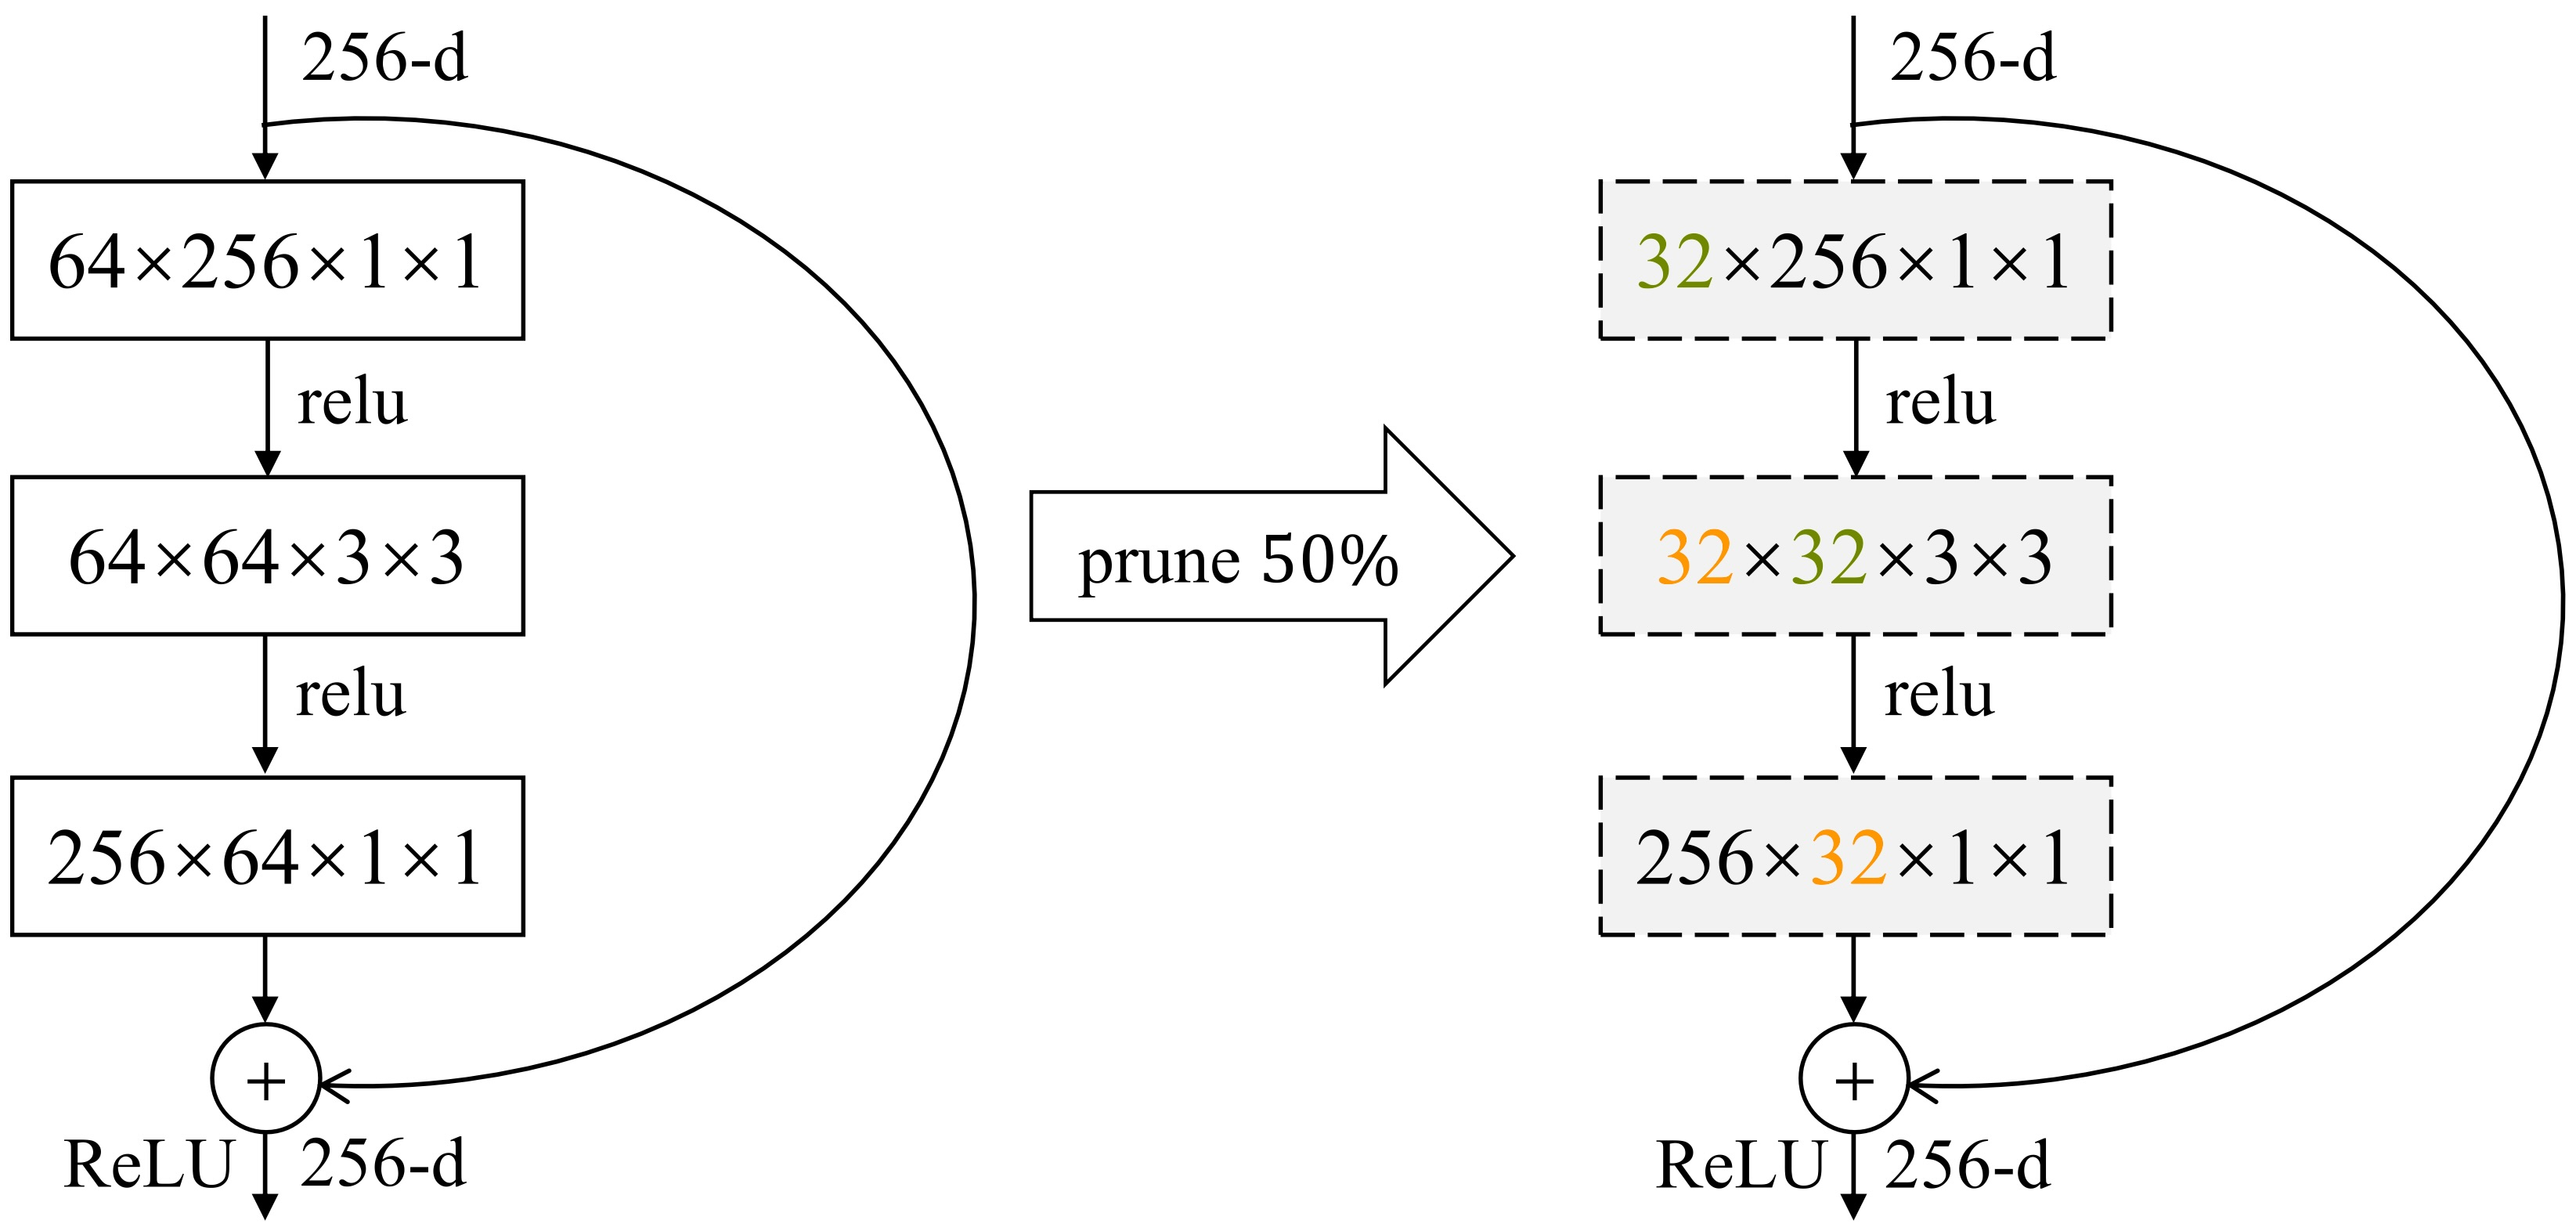
\includegraphics[width=\columnwidth]{images/resnet-pruning.png}
    \end{center}
    \caption{Pruning strategy of ResNet. The pruning is performed in such a way that the final size of the output is maintained, so that the residual connection can be added. Image from \cite{8416559}.}
    \label{fig:pruning-resnet}
\end{figure}

The use of residual connections requires pruning at the block level.
The definition of a block depends on the specific architecture of ResNet. In the case of ResNet-34, a block consists of two convolutional layers, as shown in \autoref{table:resnet}, so pruning is applied to pairs of convolutions in order to add the identity carried by the residual connection.
\newpage

\section{Knowledge distillation}
\label{sec:method-kd}

\begin{figure}[H]%
	\centering

    \begin{center}
        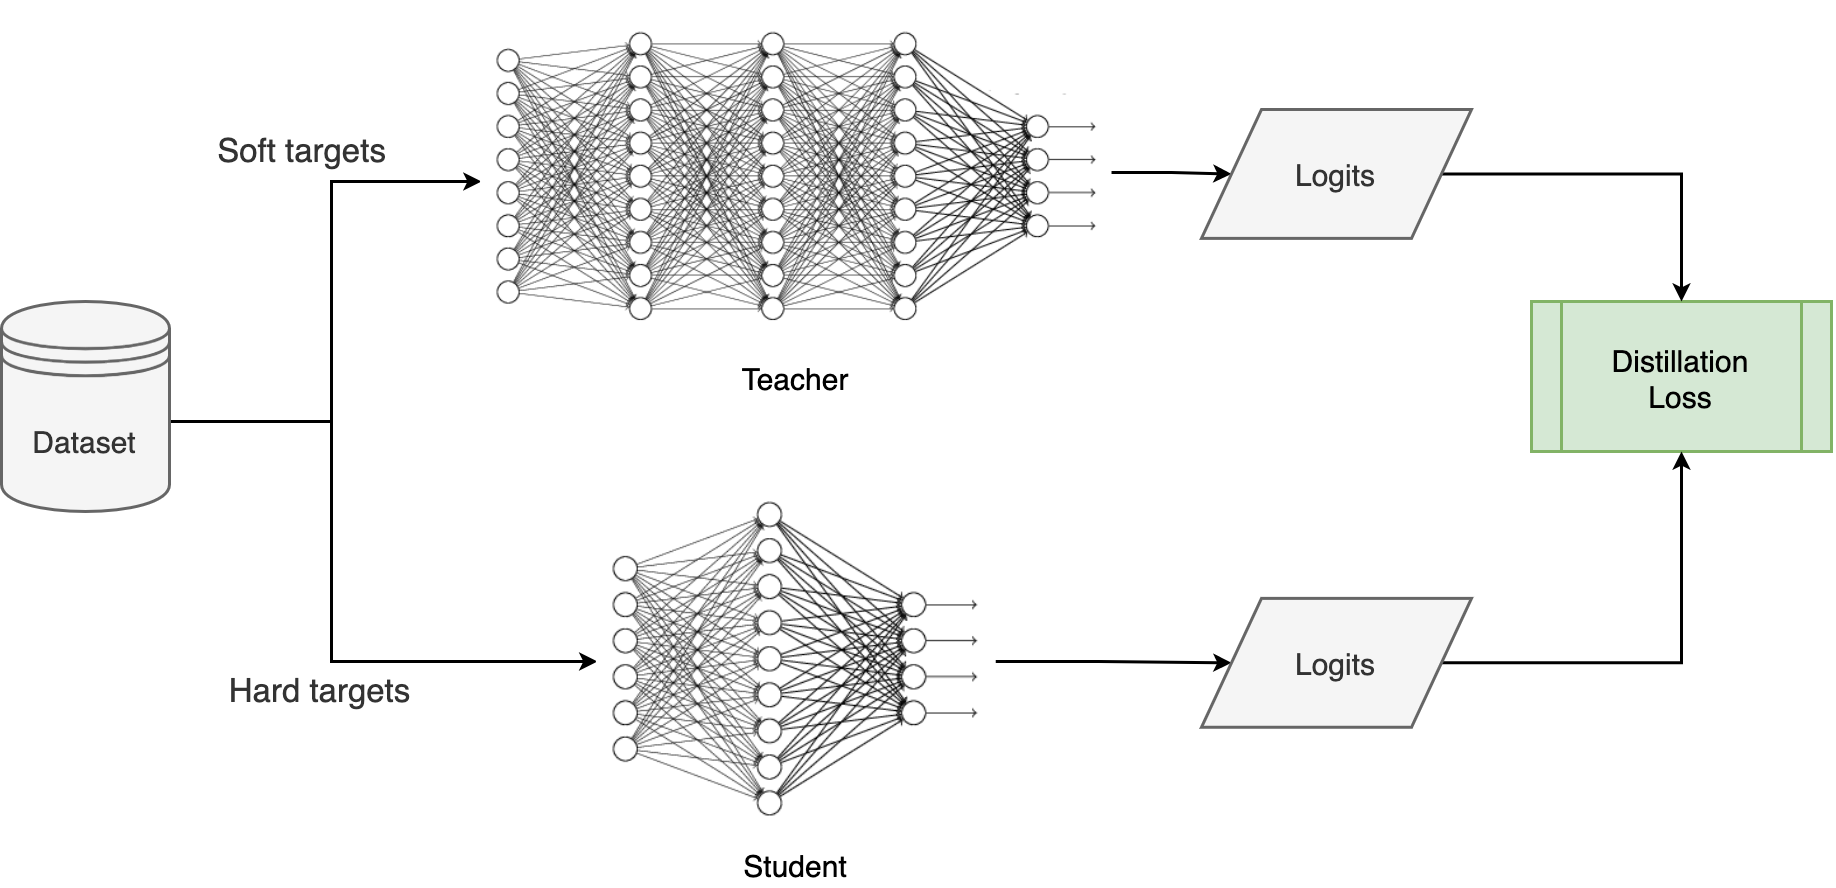
\includegraphics[width=\columnwidth]{images/kd.drawio.png}
    \end{center}

	\caption{Knowledge distillation pipeline. The student model is trained by exploiting the teacher model using the distillation loss. This loss considers both the logits of the teacher and the real data labels.}%
	\label{fig:kd}%
\end{figure}

Another approach used to tackle the problem of the large number of model parameters is Knowledge Distillation (KD) \cite{hinton2015distilling}. KD is the process of transferring knowledge from a pre-trained large model to a smaller one. Even if large models (such as very deep neural networks like ResNet-152) have higher knowledge capacity than small models, this capacity might not be fully exploited. A large model with regularization (e.g. dropout) generalizes better than a small model when trained directly on the data and labels, however, a small model can be trained to generalize better with the help of a large model. This training setting is referred to as 'teacher-student', where the smaller model is the student and it is trained to mimic the larger one which is the teacher.

As described by Gou et al. in \cite{gou2021knowledge},
Response-Based Knowledge is a type of KD which refers to the output layer of the teacher model.
In this thesis, the implementation of the KD is based on the paper of Hinton et al. in \cite{hinton2015distilling}.
The main idea is to directly mimic the final prediction
of the teacher model.
The reason behind this is that the output probabilities of a trained model give more information than the raw labels, because they assign non-zero probabilities to incorrect classes.
Knowledge is transferred from the teacher to the student using a loss function, known as the distillation loss, which captures the differences between the logits of the student and teacher models.
As the loss is reduced over time, the student becomes more accurate in making predictions similar to those of the teacher.
The teacher-student setting for KD matching the logits between the two models is shown in \autoref{fig:kd}.

The distillation loss used to train the student model is computed considering both the logits produced in output by the teacher (soft targets) and the real data labels (hard targets).
The probability $p_i$ of each class $i$, is computed by the teacher model using its logit $z_i$ as follows:
\begin{equation}
    p_i = \frac{exp(z_i)}{\sum_j exp(z_j)}
\end{equation}

The small model is trained to minimize the KL Divergence between its output probability distribution and the one of the large network.
One issue with this technique is that the probabilities assigned to incorrect classes by the large network are often very small and do not contribute to the loss.
For this reason, the logits are softened using a 'temperature' $T$ in the softmax, smoothing the probability distribution and revealing inter-class relationships learned by the teacher.
Then, the softened probability is given by:
\begin{equation}\label{eq:kd_prob}
    p_i^t = \frac{exp(\frac{z_i^t}{T})}{\sum_j exp(\frac{z_i^t}{T})}
\end{equation}
where higher values of $T$ produce softer probabilities. The prediction $p_i^t$ is called soft target, shown in \autoref{fig:kd}. 
Note that the teacher's output probability is denoted by $p_i^t$ using the letter $t$, as opposed to the student's output probability denoted by $p_i^s$ with the letter $s$.

Similarly, the \autoref{eq:kd_prob} is used to compute the class probability $p_i^s$ predicted by the student using its logit $z_i^s$ and the same temperature $T$.
In addition to the soft targets of the teacher, Hinton et al. in \cite{hinton2015distilling} show that it is beneficial to train the student model to produce the real data labels, called hard targets and shown in \autoref{fig:kd}.
Therefore, by setting $T = 1$, the student uses \autoref{eq:kd_prob} to compute the 'standard' class probability $\hat{y}_i^s$.

Thus, considering both the KL divergence of the output probability distribution, and the Cross-Entropy between $\hat{y}_i^s$ and the true data label $y_i$, the final distillation loss is given by:
\begin{equation}
    \mathcal{L}_{KD} = \alpha \left[\sum_{i=1}^{\substack{\text{output}\\\text{size}}} p_i^t \, log \left( \frac{p_i^t}{p_i^s} \right) \right]
    + (1-\alpha) \left[-\sum_{i=1}^{\substack{\text{output}\\\text{size}}} y_i^s \, (\log \hat{y}_i^s) \right]
\end{equation}
where $\alpha \in [0, 1]$ is a hyper-parameter controlling the weighted average between the two components.

\section{Proposed baseline for the classifier}
\label{sec:method-baseline}
To evaluate the CIL models and compare their performance with a model in a traditional setup, it is necessary to define a baseline.
The CIL setup is very useful for introducing new classes after training, but in general this advantage is at the expense of the model's performance. Consequently, a CIL model performs worse than a traditional one, but a good CIL algorithm should narrow this gap in performance as much as possible.

Without considering the CIL aspect, different approaches can be defined to handle a classical classification problem. This chapter discusses the different baselines introduced with the aim of comparing them with the CIL models.

\subsection{Baseline without incremental steps}
\label{sec:method-baseline1}
The most direct approach is to define a baseline using the DER algorithm.
This means taking all the classes introduced at each iteration of incremental learning and using them from the very beginning, at task 0, to train the model with the DER algorithm.
The process described above defines the first type of baseline.

Although this approach appears to be simple and straightforward, it has a problem related to what is described in \autoref{sec:method-pruning}. In fact, such an approach is not very fair, as the baseline has a number of parameters $N$ equal to the CNN used as the backbone for the feature extractor, while the CIL model trained with the DER algorithm has a number of parameters equal to $N + t \times N$ (where $t$ is the number of iterations of incremental learning).
As a result, the CIL model may perform better than the baseline only because it has a significantly larger number of parameters.

\subsection{ResNet-152 architecture}
\label{sec:method-baseline2}
To solve the problem of the first baseline definition, concerning the difference in parameters between the baseline and the CIL model, a second type of baseline is defined.
In this second approach, the DER algorithm is no more exploited, instead it is used ResNet-152 which is a network with a significantly higher number of parameters compared to ResNet-34. This is done to bridge the gap of the number of parameters between the baseline and the CIL model. The CNN based on ResNet-152 is then trained for the classification task considering all the classes.

The architecture of ResNet-152 is very similar to the one described in table \autoref{table:resnet}, in fact it maintains all the main features such as skip-connections, but has each block composed of more convolutional layers, and the number of stacked blocks increases. The architecture of ResNet-152 consists of 60 million parameters and is described in \autoref{table:resnet-152}.


\begin{table}
    \centering
    \begingroup
    
    \begin{tabular}{>{\centering\arraybackslash}p{.3\textwidth}|>{\centering\arraybackslash}p{.3\textwidth}|>{\centering\arraybackslash}p{.3\textwidth}}


        \hline
        \multicolumn{3}{c}{\textbf{ResNet-152 architecture}}\\
        \hline
        \textbf{Layer name} & \textbf{Output size} & \textbf{Layer} \\
        \hline
        \hline
        conv1 & $112 \times 122$ & $7 \times 7, 64,$ stride $2$ \\
        \hline
          & $56 \times 56$ & $3 \times 3$ max pool, stride $2$ \\
        \hline

        \[ \textrm{conv2\char`_x} \] &  \[56 \times 56 \] & \[\left[ \begin{array}{c} 1 \times 1, \, 64\\ 3 \times 3, \, 64 \\ 1 \times 1, \, 256  \end{array} \right] \times 3 \]\\
        \hline

        \[ \textrm{conv3\char`_x} \] &  \[28 \times 28 \] & \[\left[ \begin{array}{c} 1 \times 1, \, 128 \\ 3 \times 3, \, 128  \\ 1 \times 1, \, 256  \end{array}\right] \times 8 \]\\
        \hline

        \[ \textrm{conv4\char`_x} \] &  \[14 \times 14 \] & \[\left[ \begin{array}{c} 1 \times 1, \, 256\\ 3 \times 3, \, 256\\ 1 \times 1, \, 1024  \end{array}\right] \times 36 \]\\
        \hline

        \[ \textrm{conv5\char`_x} \] &  \[7 \times 7 \] & \[\left[ \begin{array}{c} 1 \times 1, \, 512\\ 3 \times 3, \, 512\\ 1 \times 1, \, 2048  \end{array}\right] \times 3 \]\\
        \hline
        & $1000 \times 1$ & average pool \\
        \hline
        FC & $1000 \times 1$ & $1000$-d FC layer, softmax \\
        \hline
        \end{tabular}
    \endgroup
    \caption{Architecture of ResNet-152, the brackets represent a stack of building blocks.}
    \label{table:resnet-152}
\end{table}

Although this new baseline is an improvement over the previous one, the number of parameters is still lower than in the CIL model, as in the case of the baseline of the first type.

\subsection{DER-based architecture}
\label{sec:method-baseline3}
The third introduced baseline solves the problem of the different number of parameters between the CIL model and the baseline.
To this purpose, referring to the exact same setup used for training the CIL model and considering the number of iterations $t$, the DER algorithm is exploited to define another neural network by performing $t$ incremental learning steps without actually training the new network.
Subsequently, since at timestamp $t$ of incremental learning the DER algorithm freezes the weights of the previous feature extractors, all weights, both related to the feature extractors $\mathcal{F}_i$ and to the classifier $\mathcal{H}_{i}$, are allowed to be trained.

This new network will serve as the baseline, and unlike the DER algorithm, the optimization process will aim to classify all the classes (intended as all those introduced incrementally during the training of the CIL model) without taking into account the auxiliary classifier $\mathcal{H}^a$ and the masks for pruning described in \autoref{sec:der-algorithm}.
\chapter{Experiments}
\label{chap:experiments}
This chapter presents the experiments designed to evaluate the system described in chapter \autoref{chap:methods}.
The chapter is structured as follows: \autoref{sec:exp-setup} specifies the setup used for the class incremental learning task; \autoref{sec:exp-cil} discusses the experiments related to the CIL model and \autoref{sec:exp-det} those related to the logo detector; \autoref{sec:exp-kd} describes the experiments relative to the KD; finally, \autoref{sec:exp-end2end} presents the results of experiments combining the logo detector with the CIL classifier.

\section{Setup}
\label{sec:exp-setup}
The developed system is tested considering two different CIL setups: in the first setup, the system is tested on a subset of 100 classes out of the total 2993 in the dataset; in the second setup, the model's scaling capabilities are tested considering the entire dataset. Specifically, the CIL configuration is the following:
\begin{enumerate}
    \item \textbf{100 Classes}: 100 classes are extracted from the initial dataset. For the experiments, a distinction is made between the case in which these classes are extracted randomly or are taken the 100 classes with the highest number of images.
    
    Out of these 100 classes, 30 are used for the initial task, then the remaining 70 classes are added 10 at a time through 7 incremental learning iterations.

    \item \textbf{2993 Classes (entire dataset)}: for experiments which consider the entire dataset, the first 1000 classes are used for the initial task, then follows 8 iterations of incremental learning, each adding 250 new classes.
\end{enumerate}

The train, validation and test set are built from the individual classes. For each of these, the instances are divided as follows:
\begin{itemize}
    \item \textbf{Train set}: 70 \%
    \item \textbf{Validation set}: 10 \%
    \item \textbf{Test set}: 20 \%
\end{itemize}


\section{Classifier: CIL model}
\label{sec:exp-cil}
Top-k accuracy is used to evaluate the performance of the CIL model, focusing on cases with $k=1$ and $k=5$.
Using this performance metric, a classification is considered correct if the label is present among the first $k$ predictions to which the model assigns the highest probability. Thus, the accuracy is calculated as the percentage of the correct predictions.

\subsection{100 Classes}
\subsubsection{100 Classes randomly sampled}
For the first experiments, the 100 classes are randomly sampled from the 2993 classes in the dataset, then the classifier is evaluated on the test set according to the CIL setup described in \autoref{sec:exp-setup}. 

As detailed in \autoref{sec:der-algorithm}, the DER algorithm saves some examples of the 'old' classes and reuses these examples during incremental learning iterations. In the following experiments, the memory dedicated to each old class is of 100 samples.

The first group of experiments aims to compare two types of architecture: ResNet-34 and ResNet-50. In addition, the cases where CNNs are pre-trained on ImageNet or not are also considered. For these experiments, the optimizer is SGD and neither regularization of the model via the dropout layer nor data augmentation is used.

The results of the experiments in picture \autoref{fig:exp1} and table \autoref{table:exp1}, reporting the top-1 and top-5 accuracy of the models at varying CIL tasks on the test set, show that pre-trained CNNs perform better, but there is not much difference between ResNet-34 and ResNet-50. For this reason, the architecture chosen for the experiments to follow is ResNet-34, so as to have a slightly smaller network than ResNet-50, and the network is pre-trained on ImageNet.

\begin{figure}[H]
    \centering
	\subfloat[\centering Top-1 accuracy]{{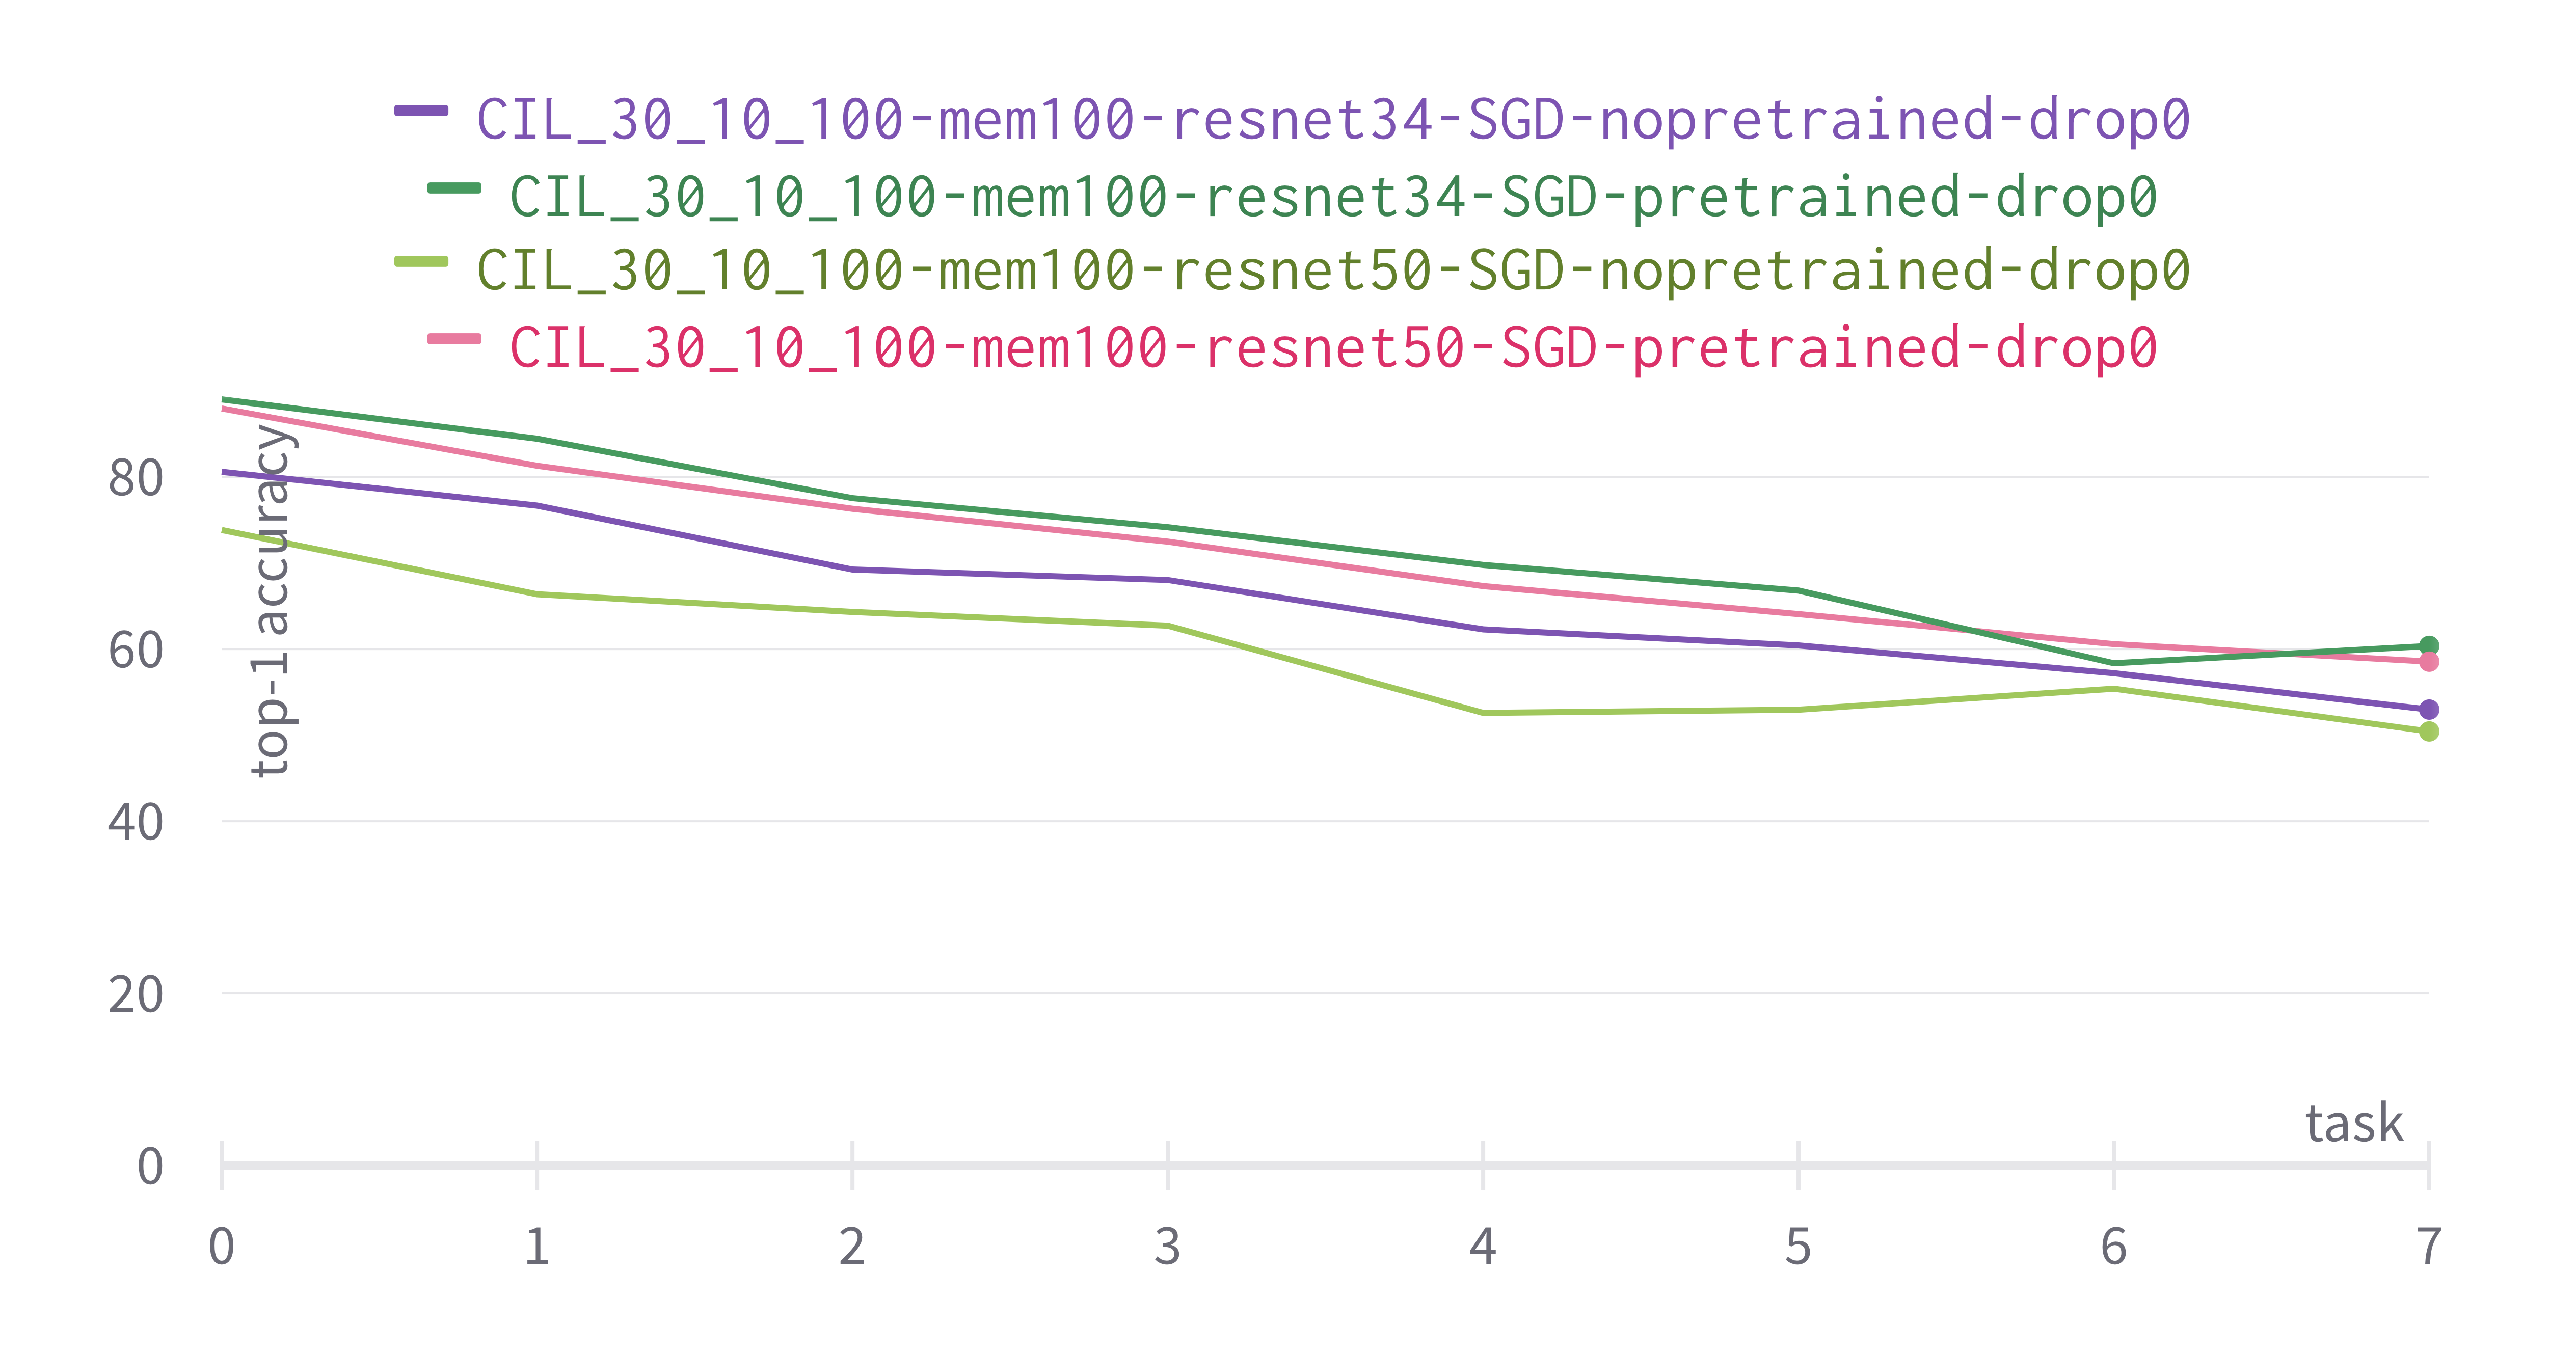
\includegraphics[width=0.80\textwidth]{images/exp/exp1-top1.png} }}%
    \qquad
    \subfloat[\centering Top-5 accuracy]{{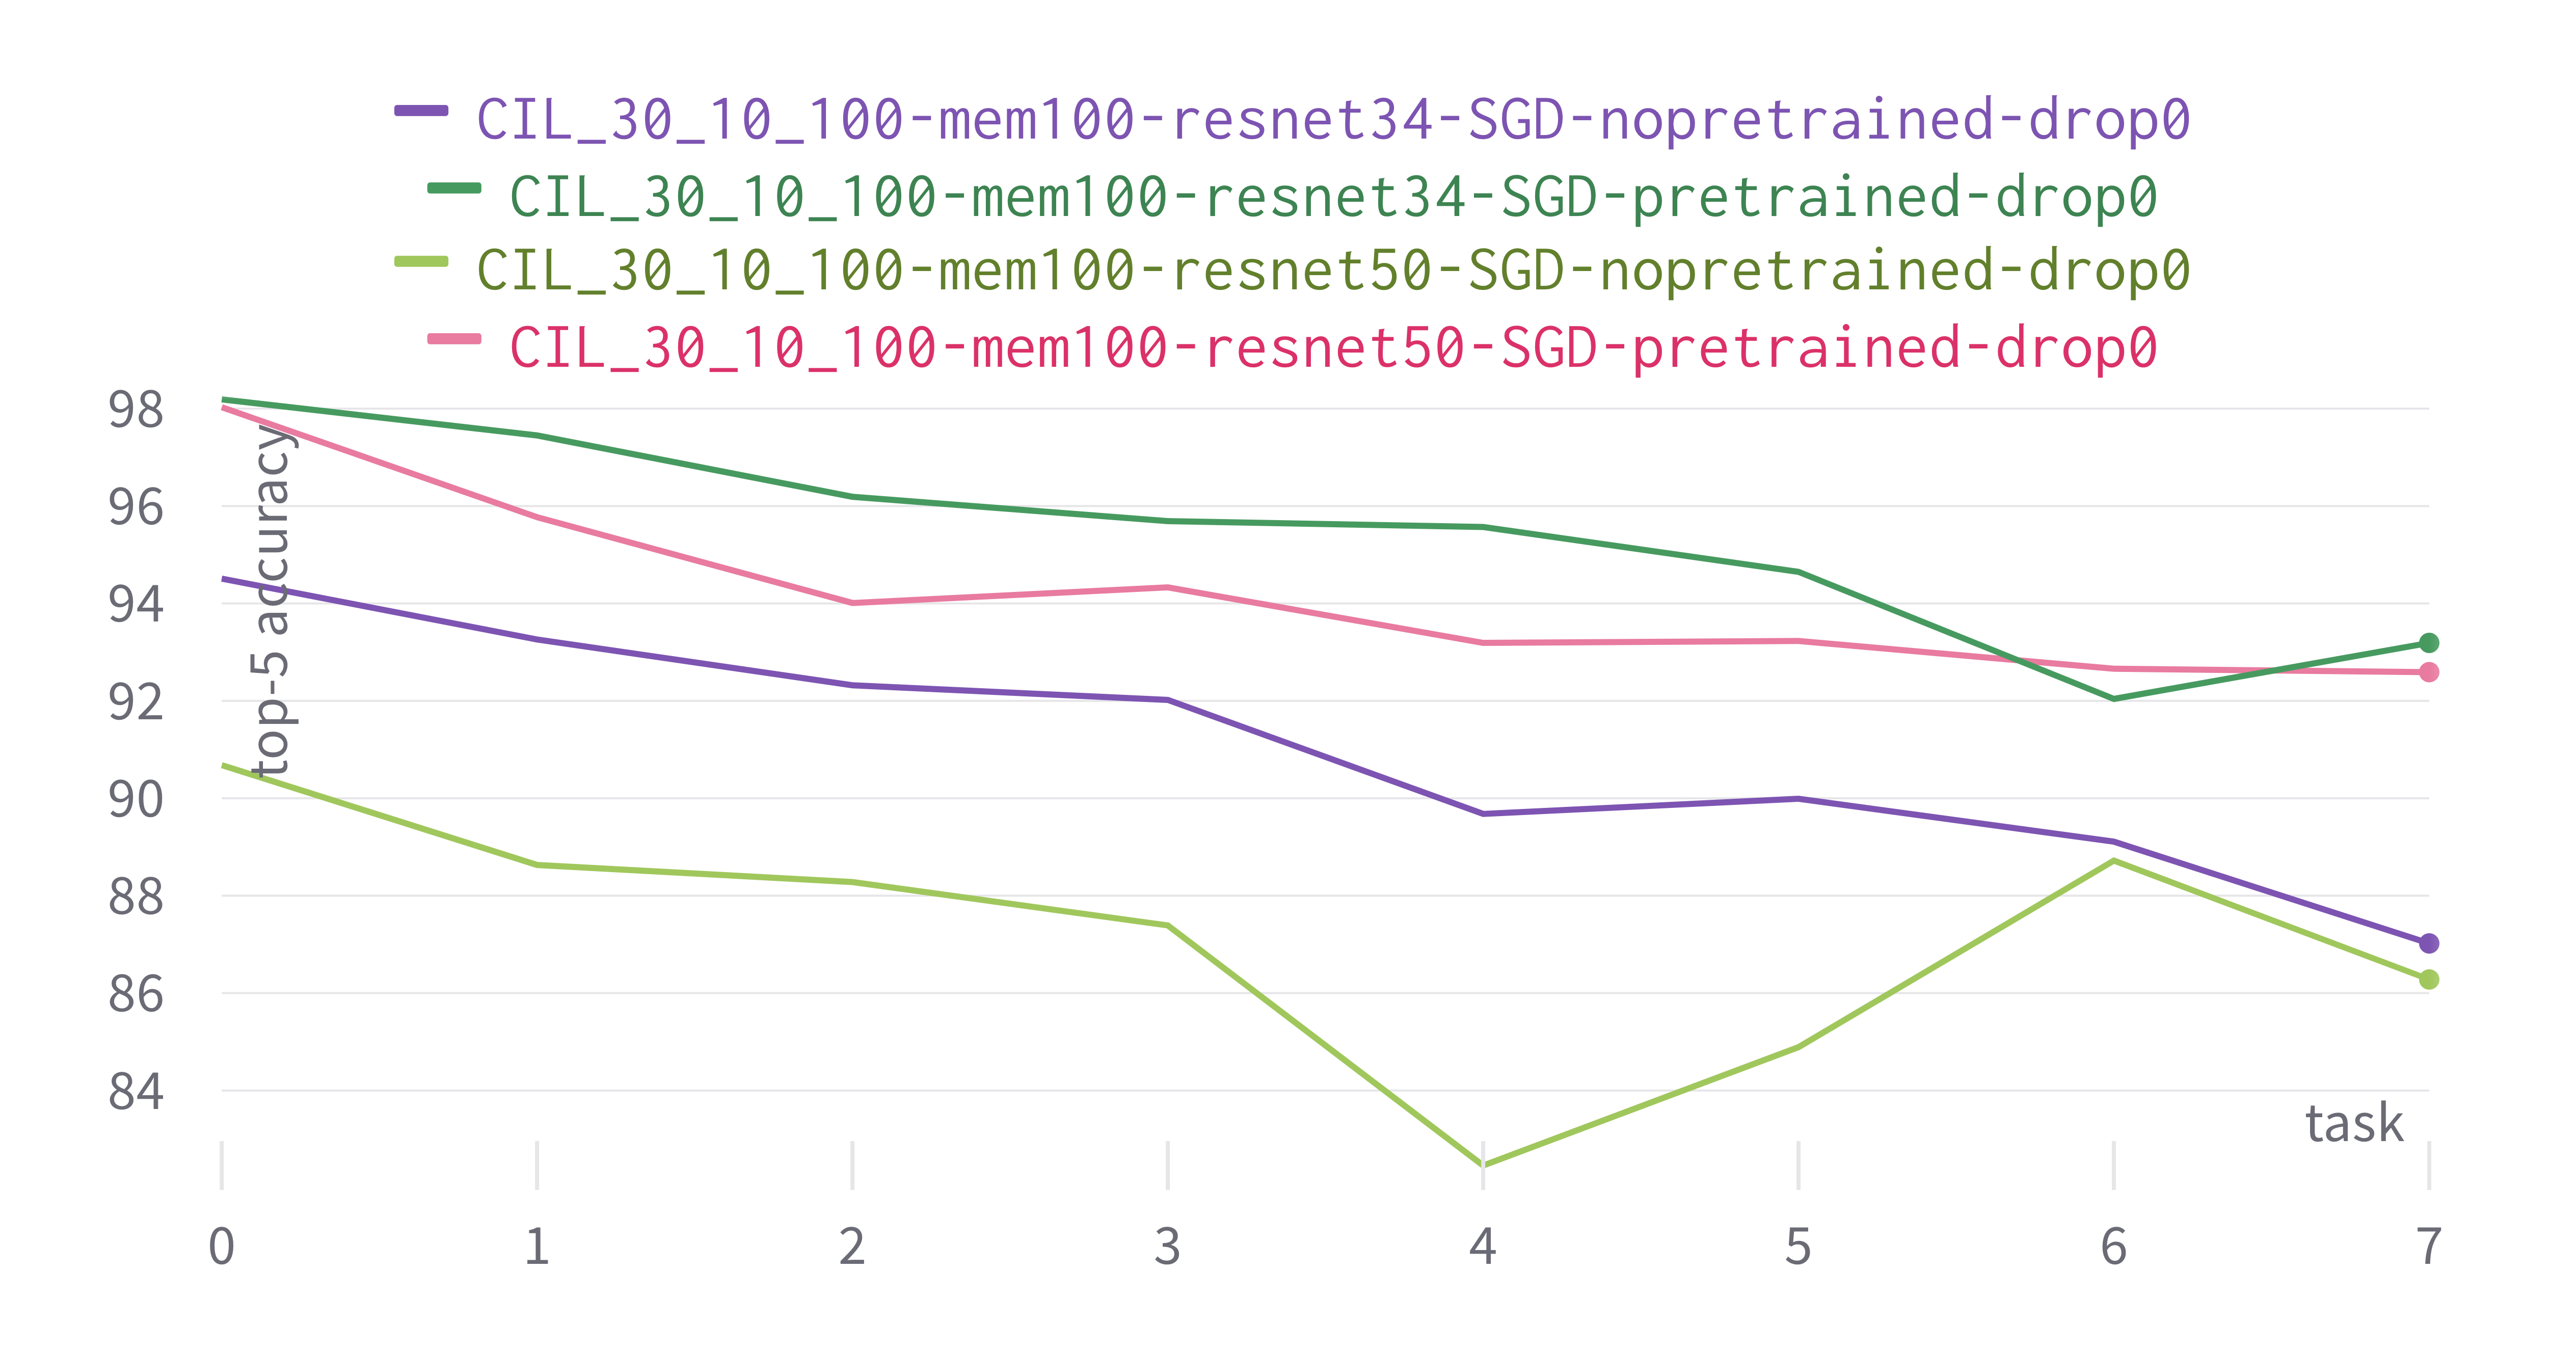
\includegraphics[width=0.80\textwidth]{images/exp/exp1-top5.png} }}%
    \caption{Top-1 and Top-5 accuracy of the models at varying CIL tasks on the test set.}%
	\label{fig:exp1}%
\end{figure}

\begin{table}[H]
    \centering
    \centerline{
    \begin{tabular}{c|c|c|c|c}
        \hline
        \textbf{Model} &
        \textbf{Backbone} &
        \textbf{Pre-trained} &
        \textbf{Top-1} & 
        \textbf{Top-5} \\
        \textbf{name} &
        &
        &
        \textbf{acc. (\%)} & 
        \textbf{acc. (\%)} \\
        \hline
        \hline
resnet34-SGD-nopretrained-drop0 &ResNet-34&no& 52.97 & 87.02\\
resnet34-SGD-pretrained-drop0 &ResNet-34&yes& \textbf{60.37} & \textbf{93.19}\\
resnet50-SGD-nopretrained-drop0 &ResNet-50&no& 50.43 & 86.28\\
resnet50-SGD-pretrained-drop0 &ResNet-50&yes& 58.54 & 92.59\\
        \hline        
    \end{tabular}}
    \caption{Top-1 and Top-5 accuracy of the models at task 7.}
    \label{table:exp1}
\end{table}


Other useful insights can be derived from the training history of a task (e.g. Task 7) which reports the top-1 accuracy on the training and validation set. In fact, as we can see from \autoref{fig:exp1-train_val} the accuracy on the training set is much higher than the validation set, which is a clear sign of overfitting of the model.

\begin{figure}[H]
    \centering
    \subfloat[\centering Accuracy on the training set]{{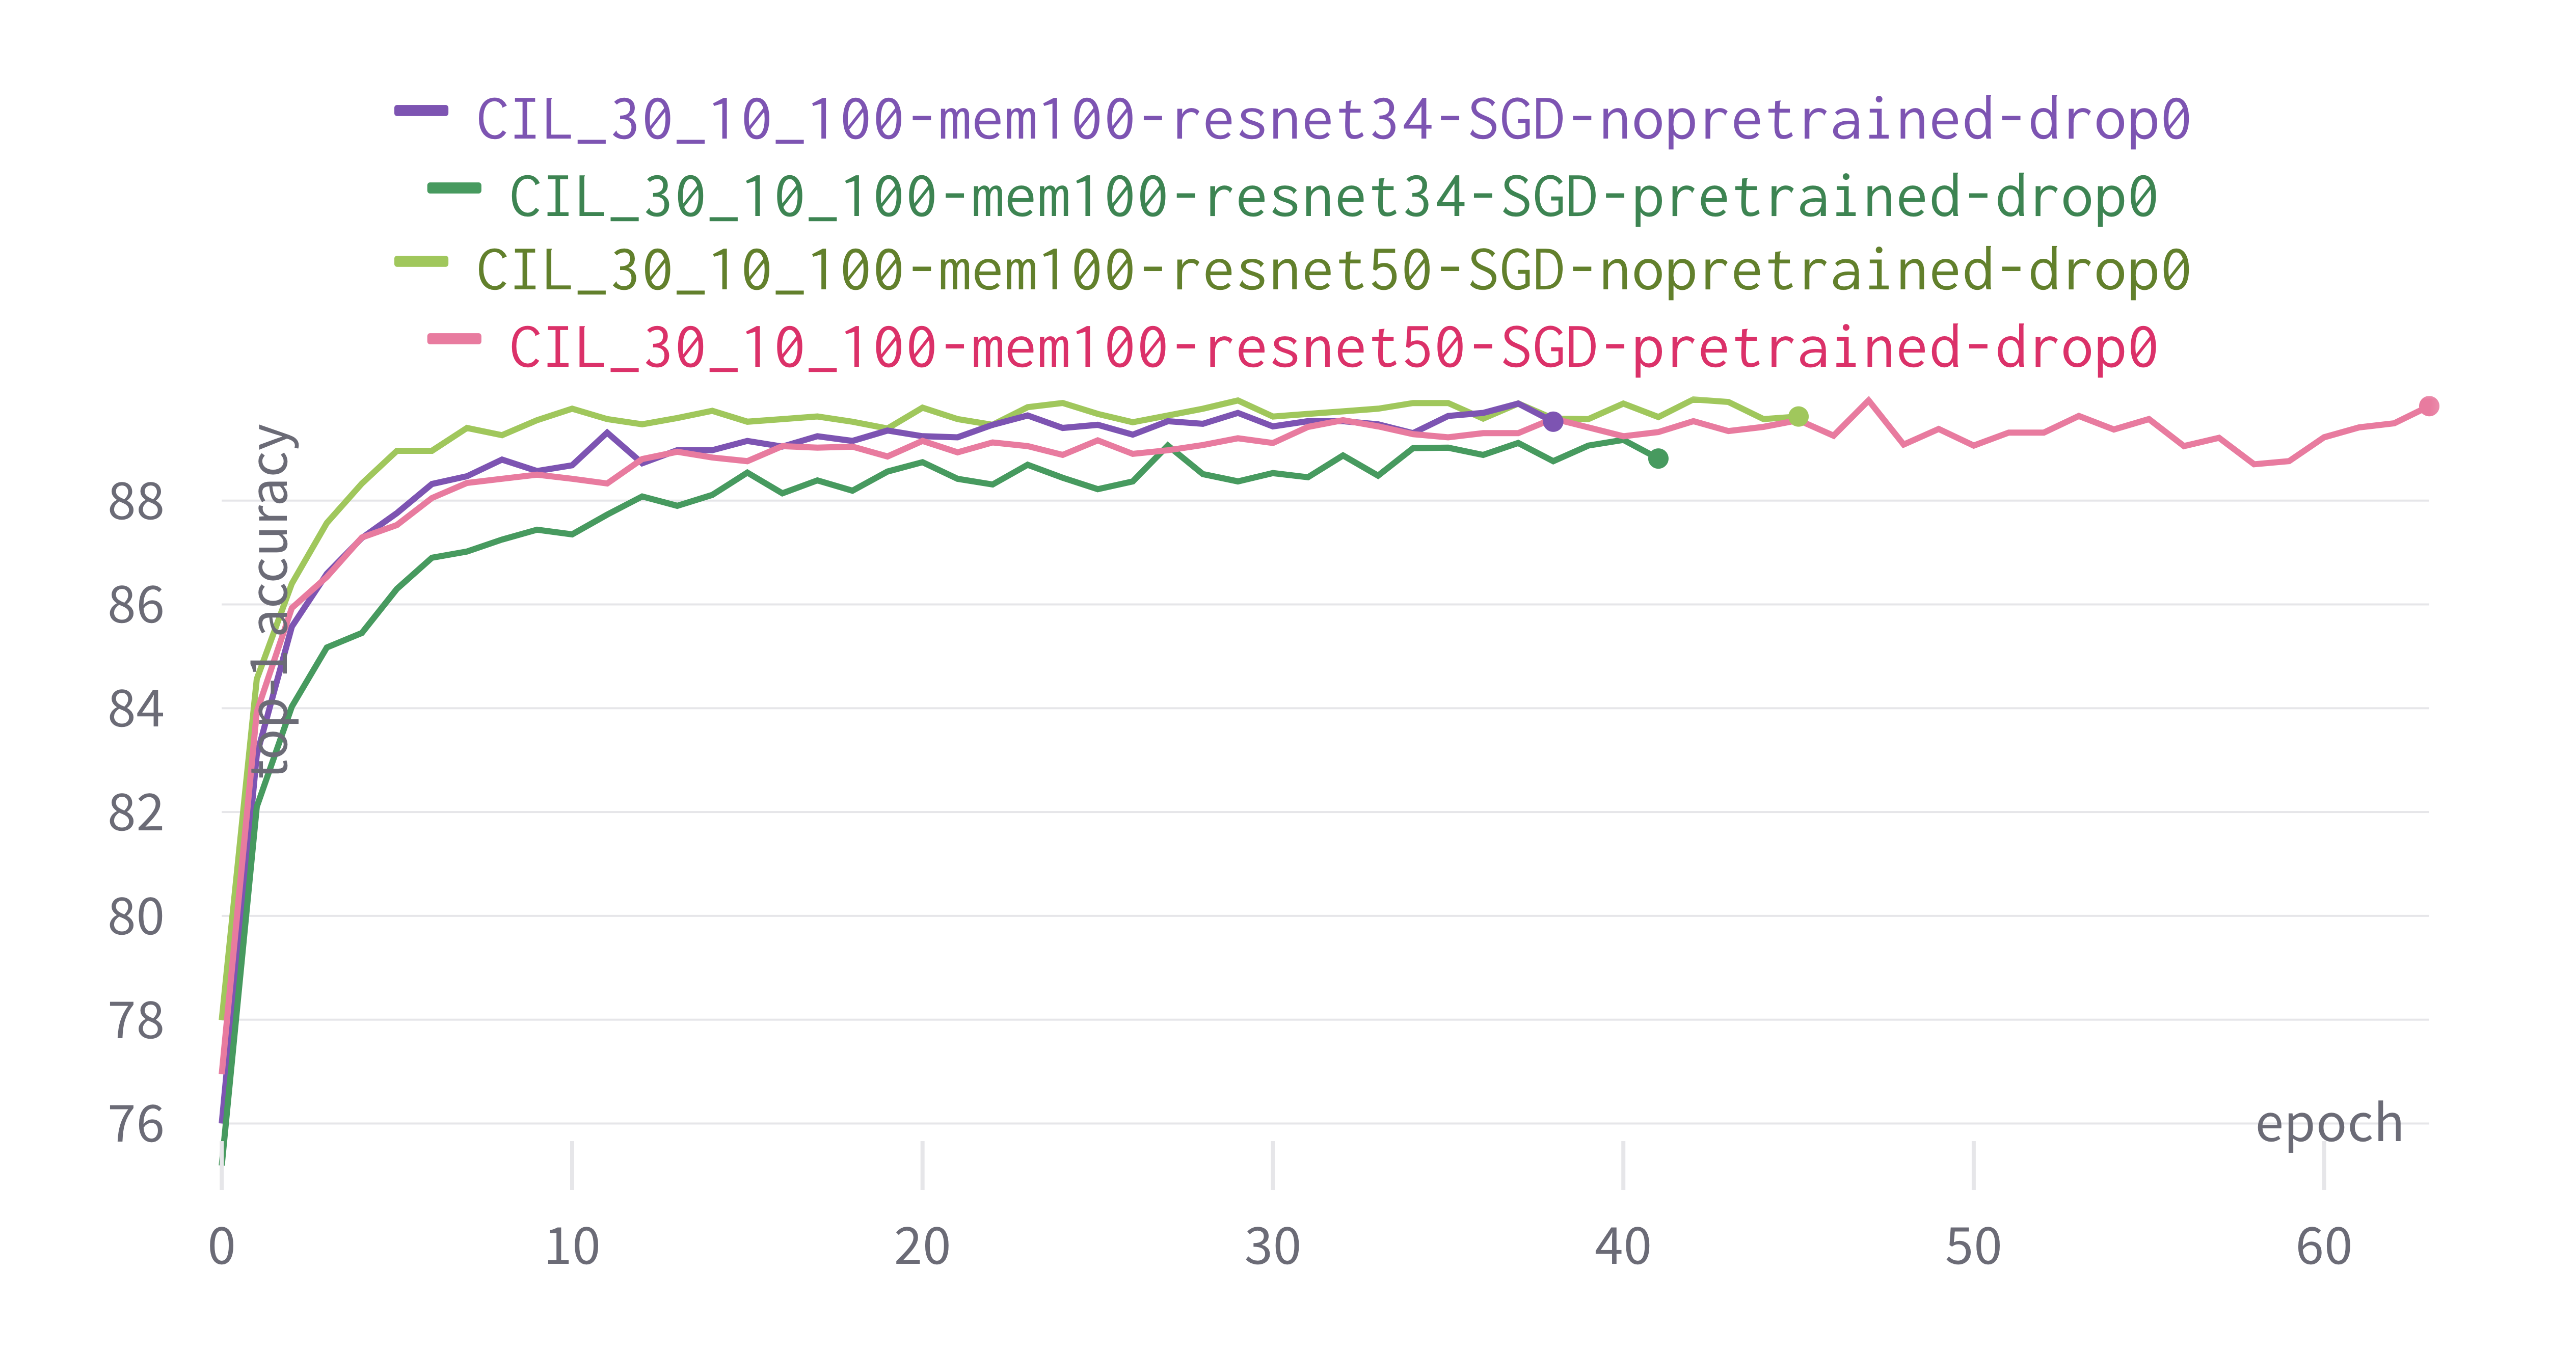
\includegraphics[width=0.80\textwidth]{images/exp/exp1-train.png} }}%
    \qquad
    \centering
    \subfloat[\centering Accuracy on the validation set]{{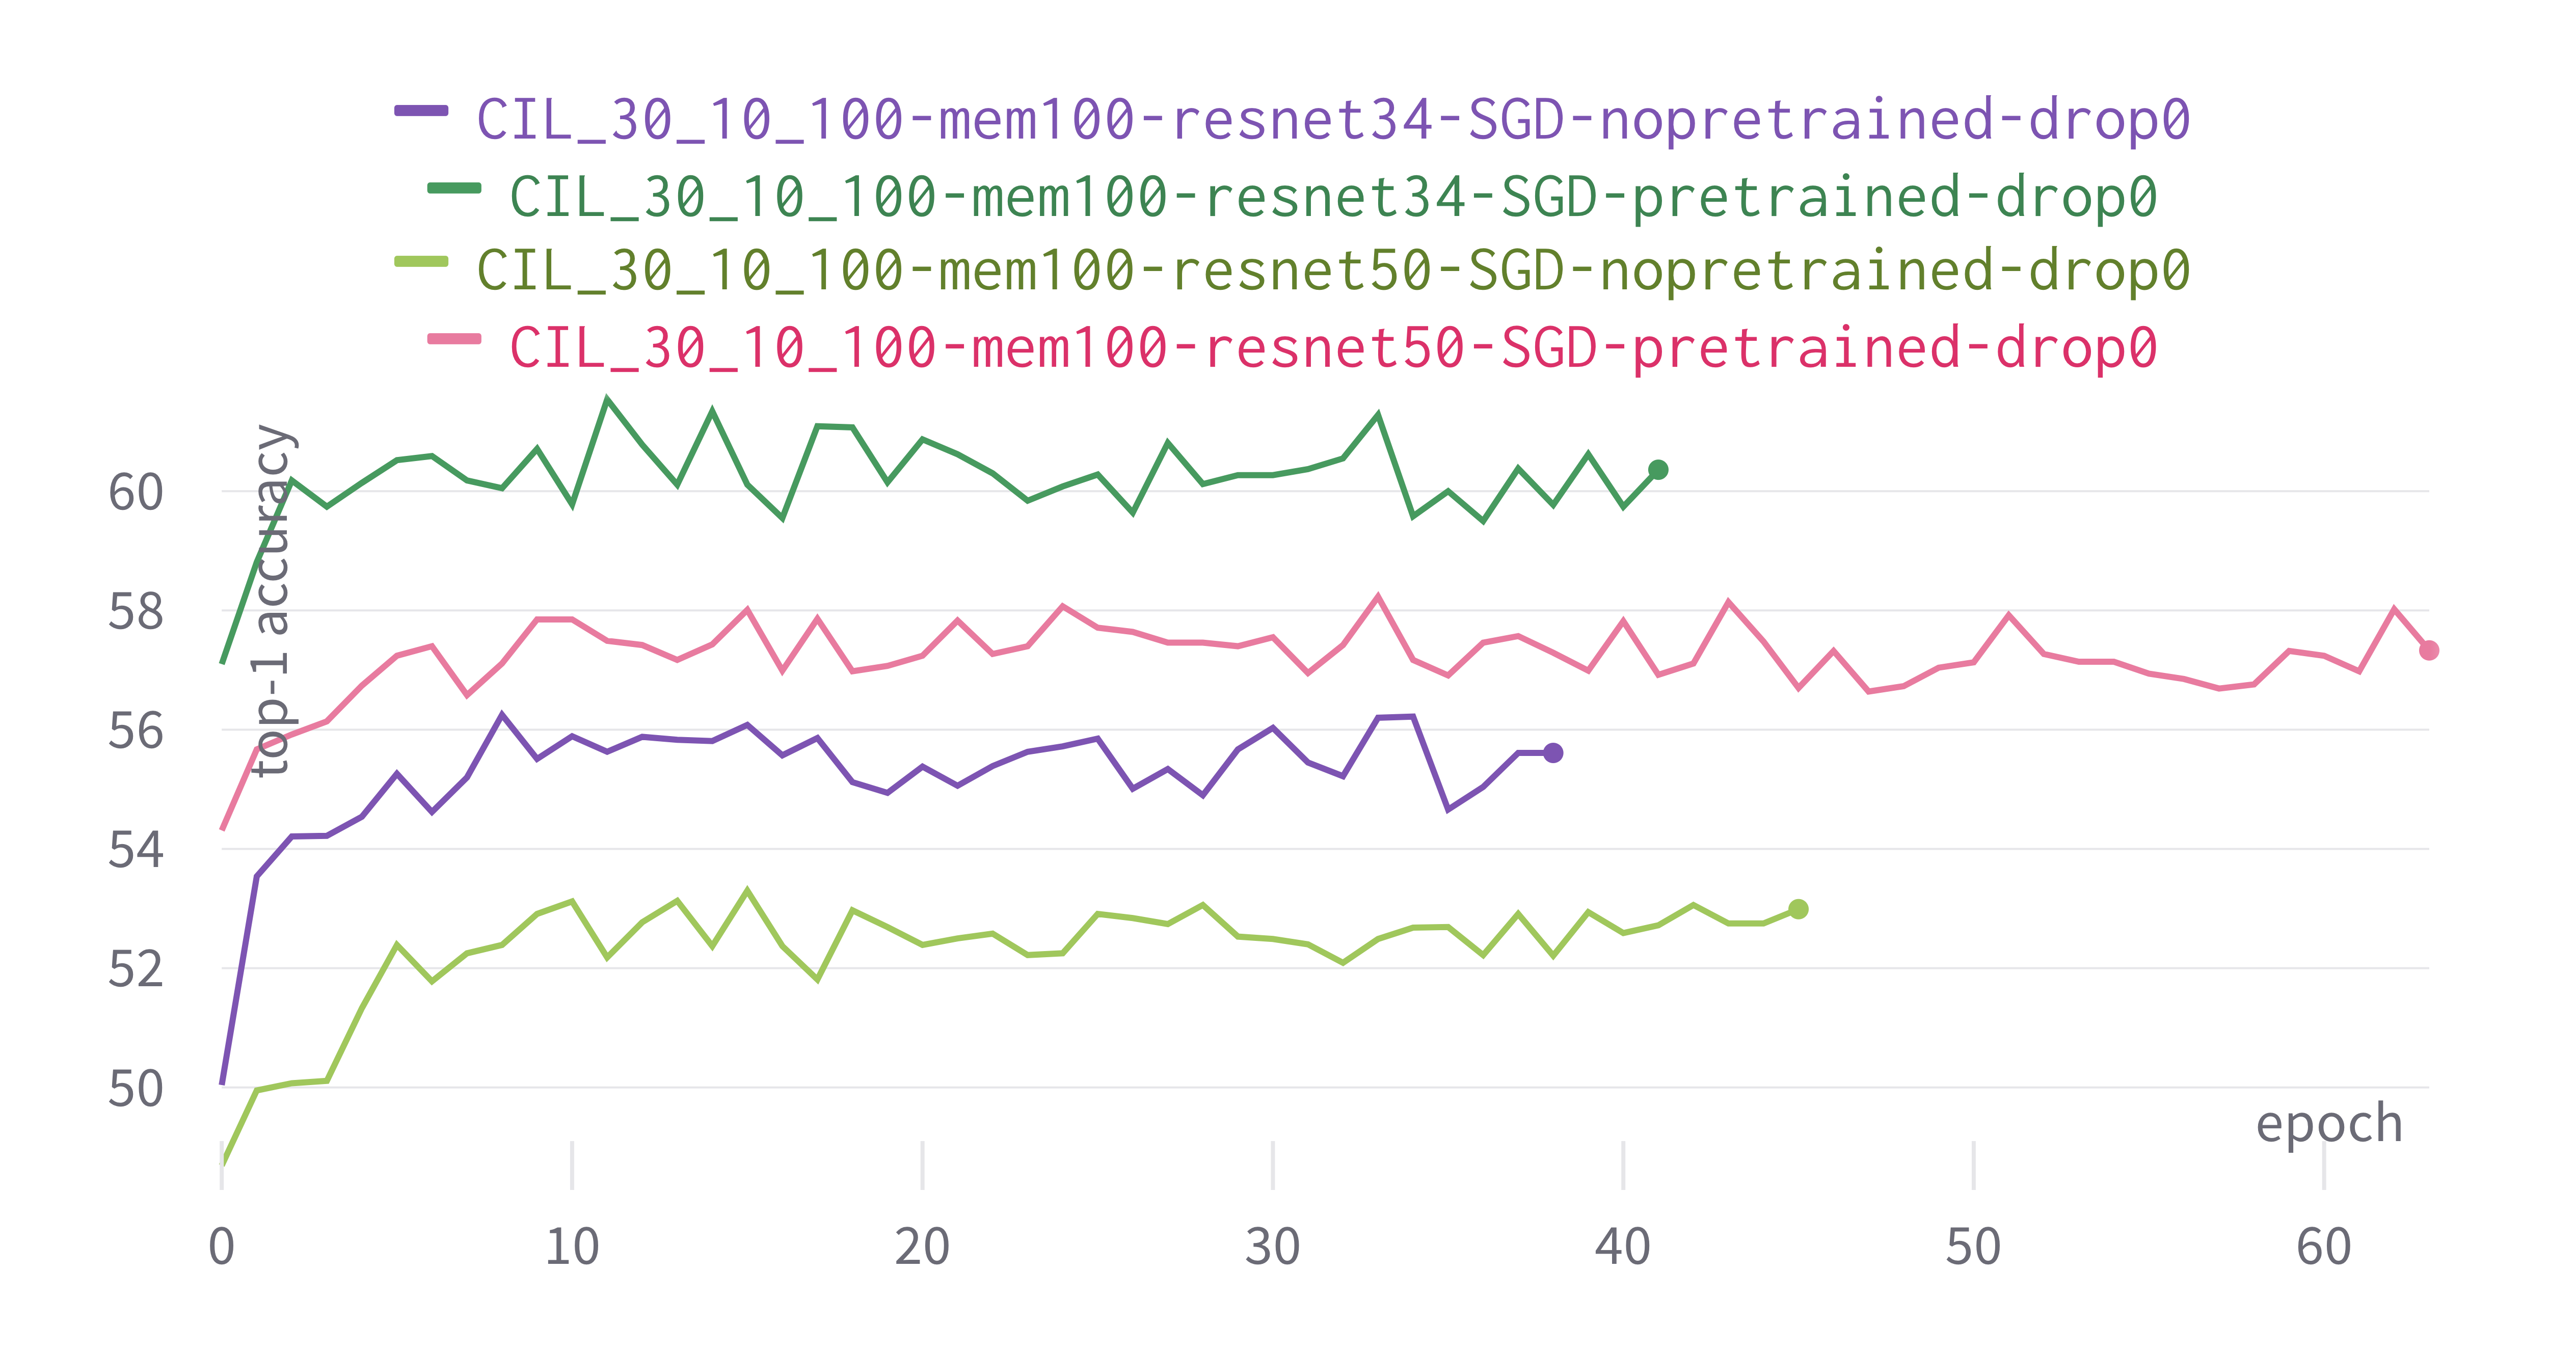
\includegraphics[width=0.80\textwidth]{images/exp/exp1-val.png} }}%
    \caption{Comparison of the accuracy at each training epoch at task 7 between the training and validation set.}%

        \label{fig:exp1-train_val}%
\end{figure}

\newpage
\subsubsection{Regularization and data augmentation}
Following the analysis discussed above, it is necessary to regularize the model.
To do so, the next experiments are performed using the dropout layer (see \autoref{sec:methods-dropout}) and data augmentation (see \autoref{sec:methods-augment}). As said before, the backbone of each model is ResNet-34 and each one is pre-trained on ImageNet.

As expected, the performance at each task is higher than before, as shown in \autoref{fig:exp2}. Analyzing \autoref{fig:exp2-train_val}, the accuracy on the train and validation set at task 7 (the same as before), the training accuracy is lower than models without regularization, but the validation accuracy is higher. This is a sign that the regularization works as intended.

As shown in \autoref{table:exp2}, the top-1 accuracy of the best regularized model which adopting data augmentation is 7\% higher than that without regularization and data augmentation.


\begin{table}[H]
    \centering
    \centerline{
    \begin{tabular}{c|c|c|c|c}
        \hline
        \textbf{Model} &
        \textbf{Data} &
        \textbf{Dropout} &
        \textbf{Top-1} & 
        \textbf{Top-5} \\
        \textbf{name} &
        \textbf{augm.} &
        \textbf{rate} &
        \textbf{acc. (\%)} & 
        \textbf{acc. (\%)} \\
        \hline
        \hline
SGD-nopretrained-drop0 &no&0.0& 52.97 & 87.02\\
SGD-pretrained-drop0 &no&0.0& 60.37 & 93.19\\
\hline
SGD-pretrained-drop0.1-augmented&yes&0.1&	67.17&\textbf{98.15}\\
SGD-pretrained-drop0.3-augmented&yes&0.3&\textbf{67.28}&	97.3\\
SGD-pretrained-drop0.5-augmented&yes&0.5&65.57&	96.24\\
        \hline        
    \end{tabular}}
    \caption{Regularized models with data augmentation. Top-1 accuracy at task 7.}
    \label{table:exp2}
\end{table}

\newpage
\begin{figure}[H]
	\centering
	\subfloat[\centering Top-1 accuracy]{{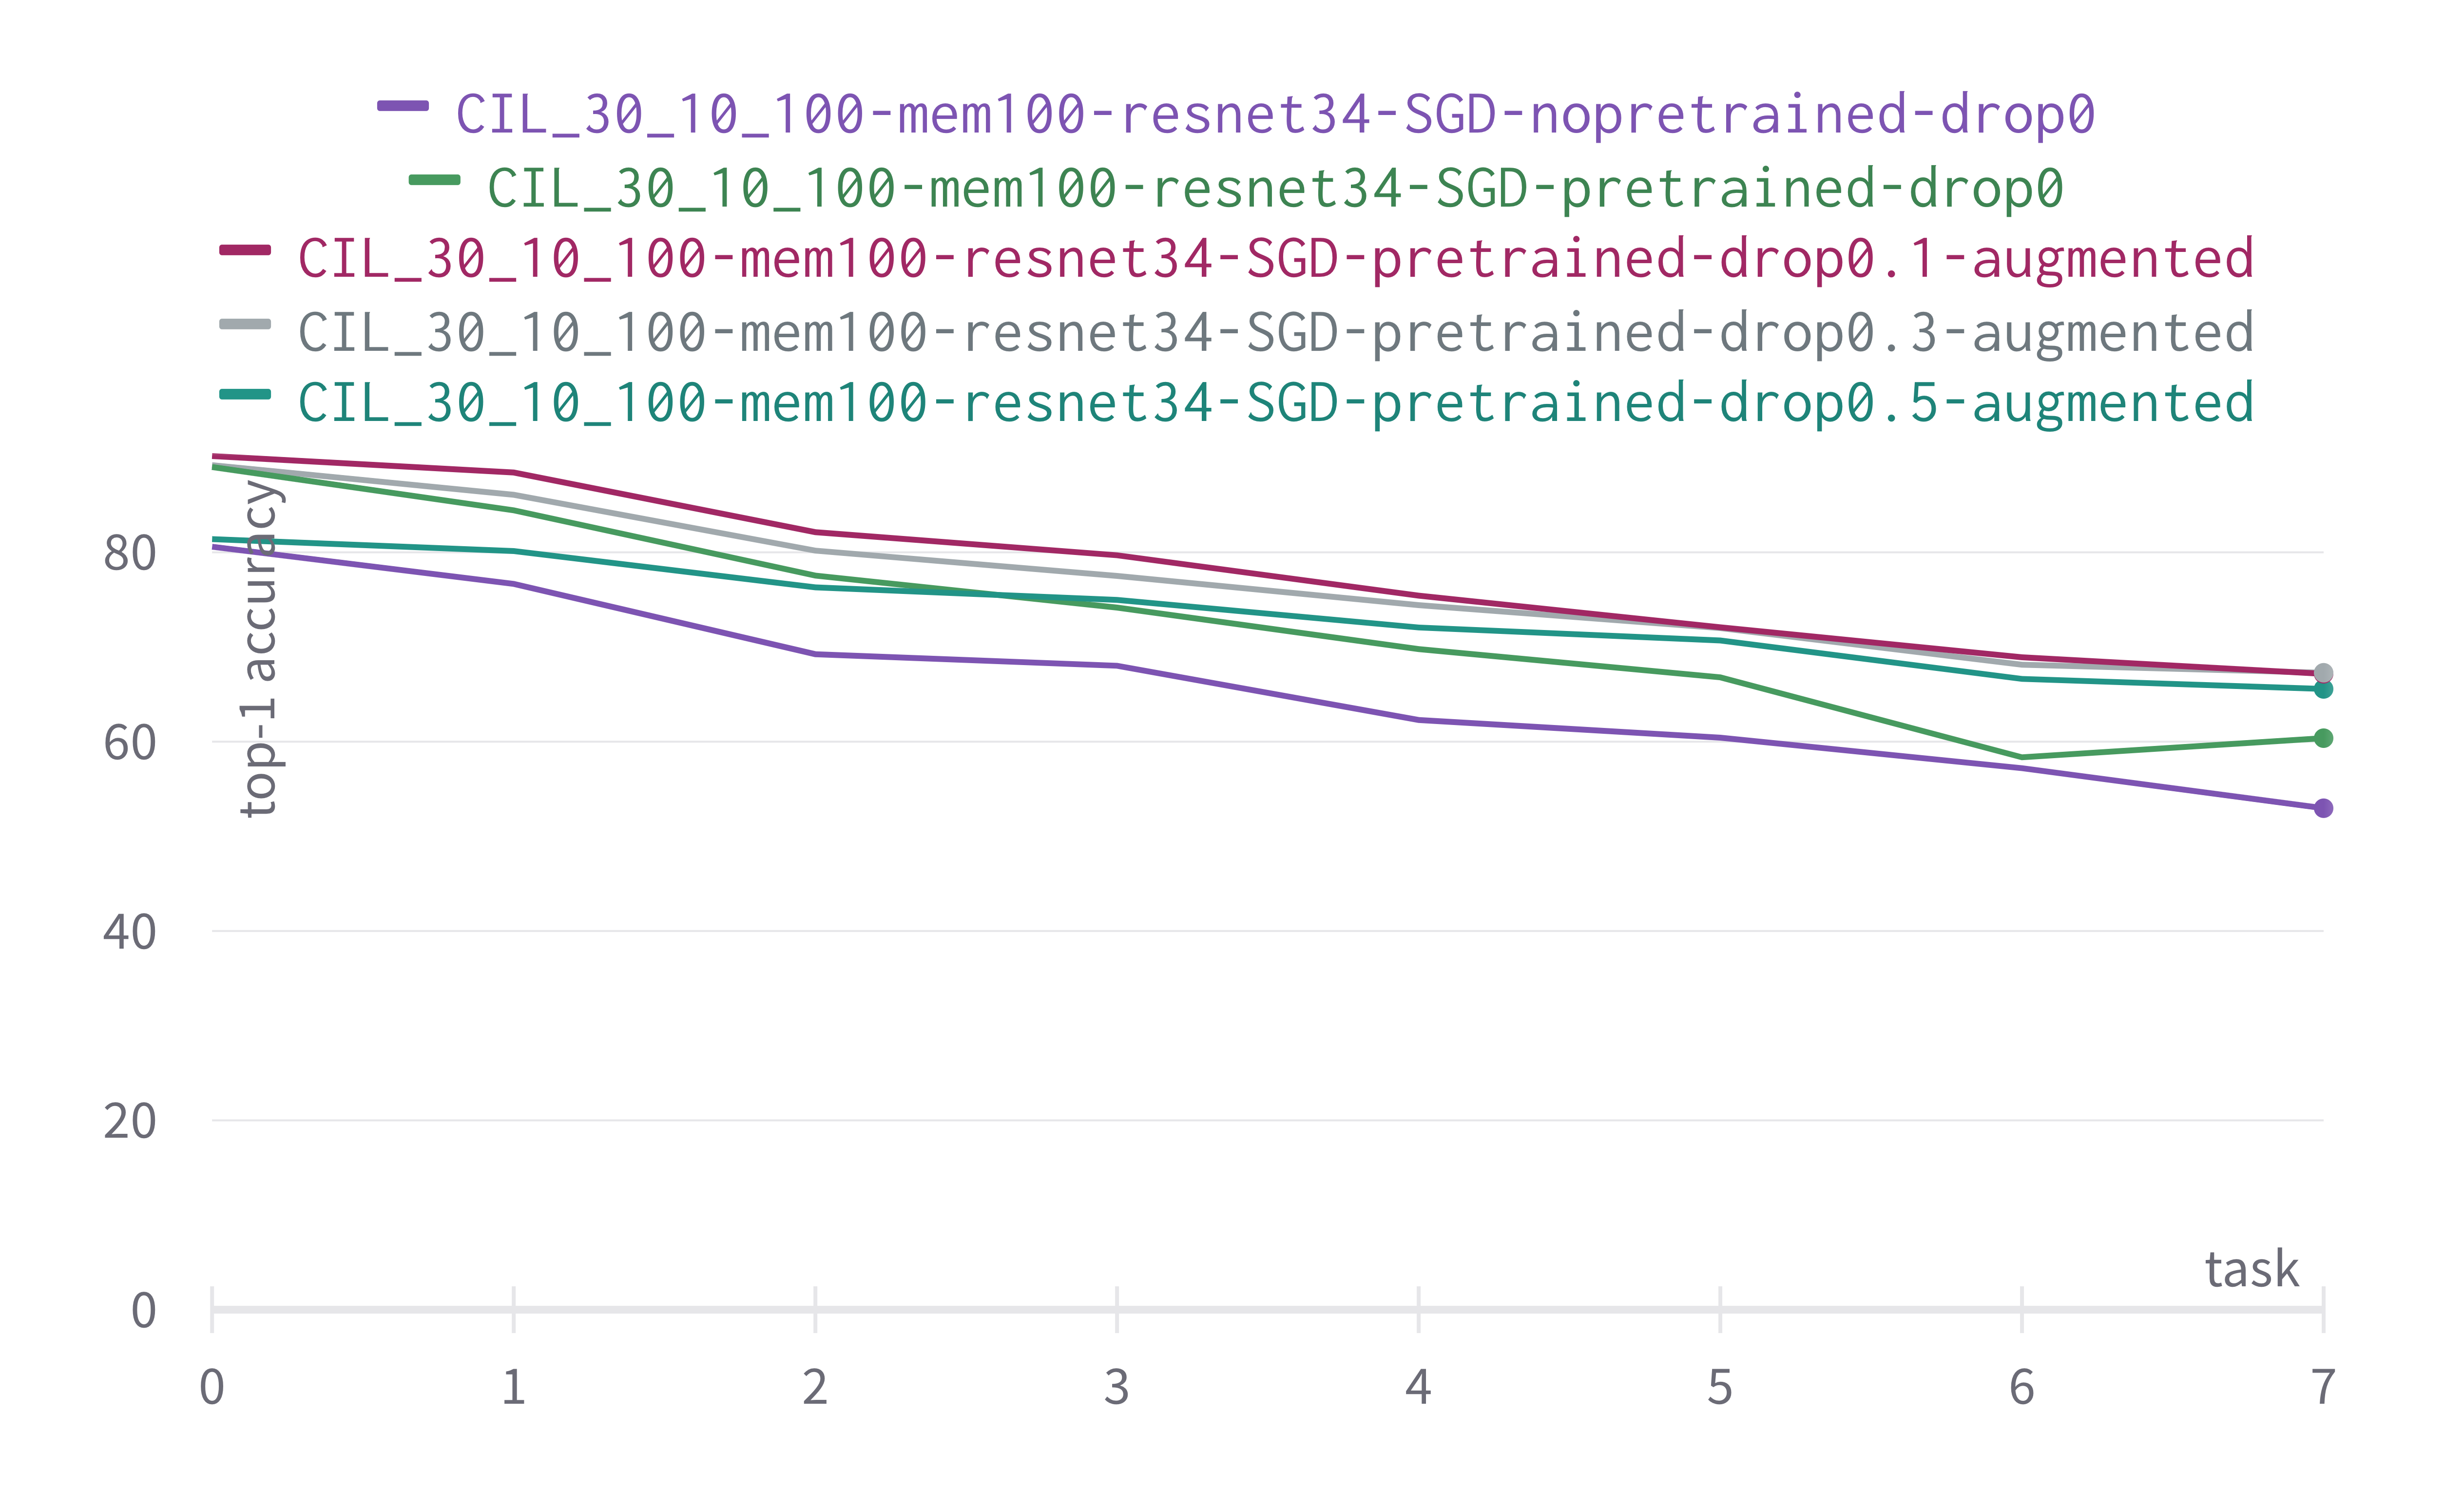
\includegraphics[width=0.80\textwidth]{images/exp/exp2-top1.png} }}%
    \qquad
	\subfloat[\centering Top-5 accuracy]{{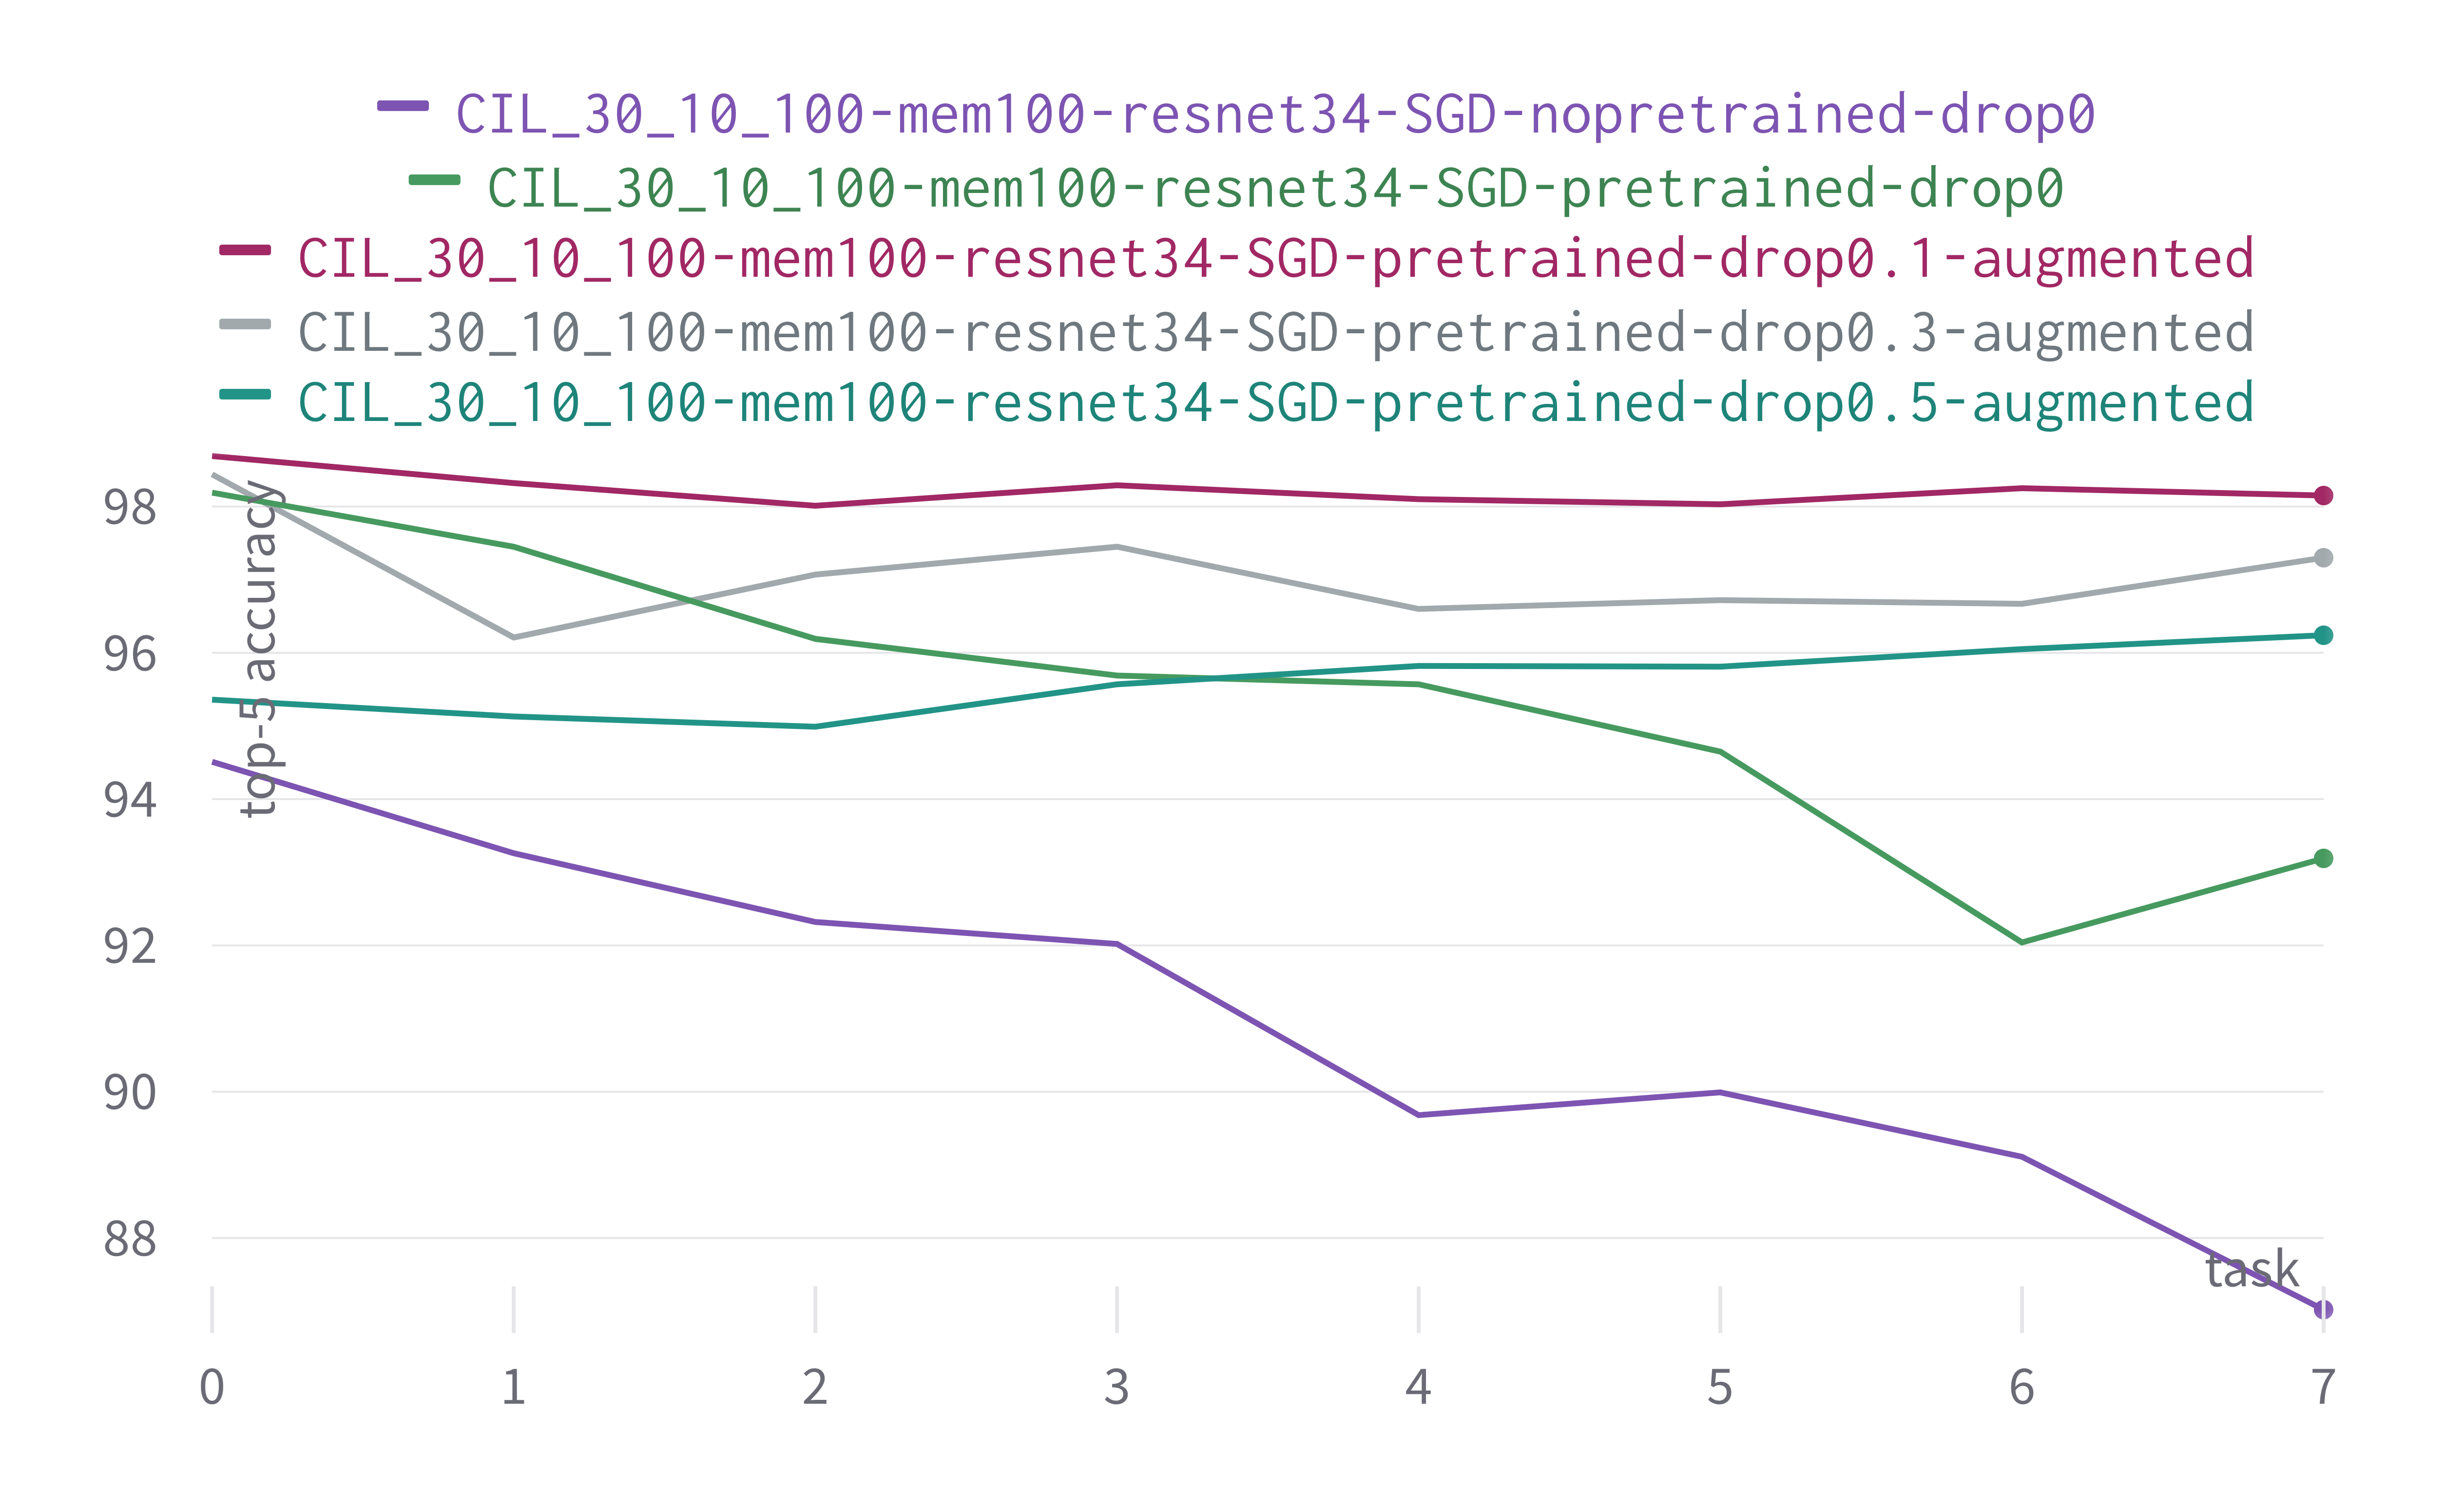
\includegraphics[width=0.80\textwidth]{images/exp/exp2-top5.png} }}%
	\caption{Top-1 and Top-5 accuracy of the regularized models using data augmentation.}%
	\label{fig:exp2}%
\end{figure}

\begin{figure}[H]
	\centering
	\subfloat[\centering Accuracy on the training set]{{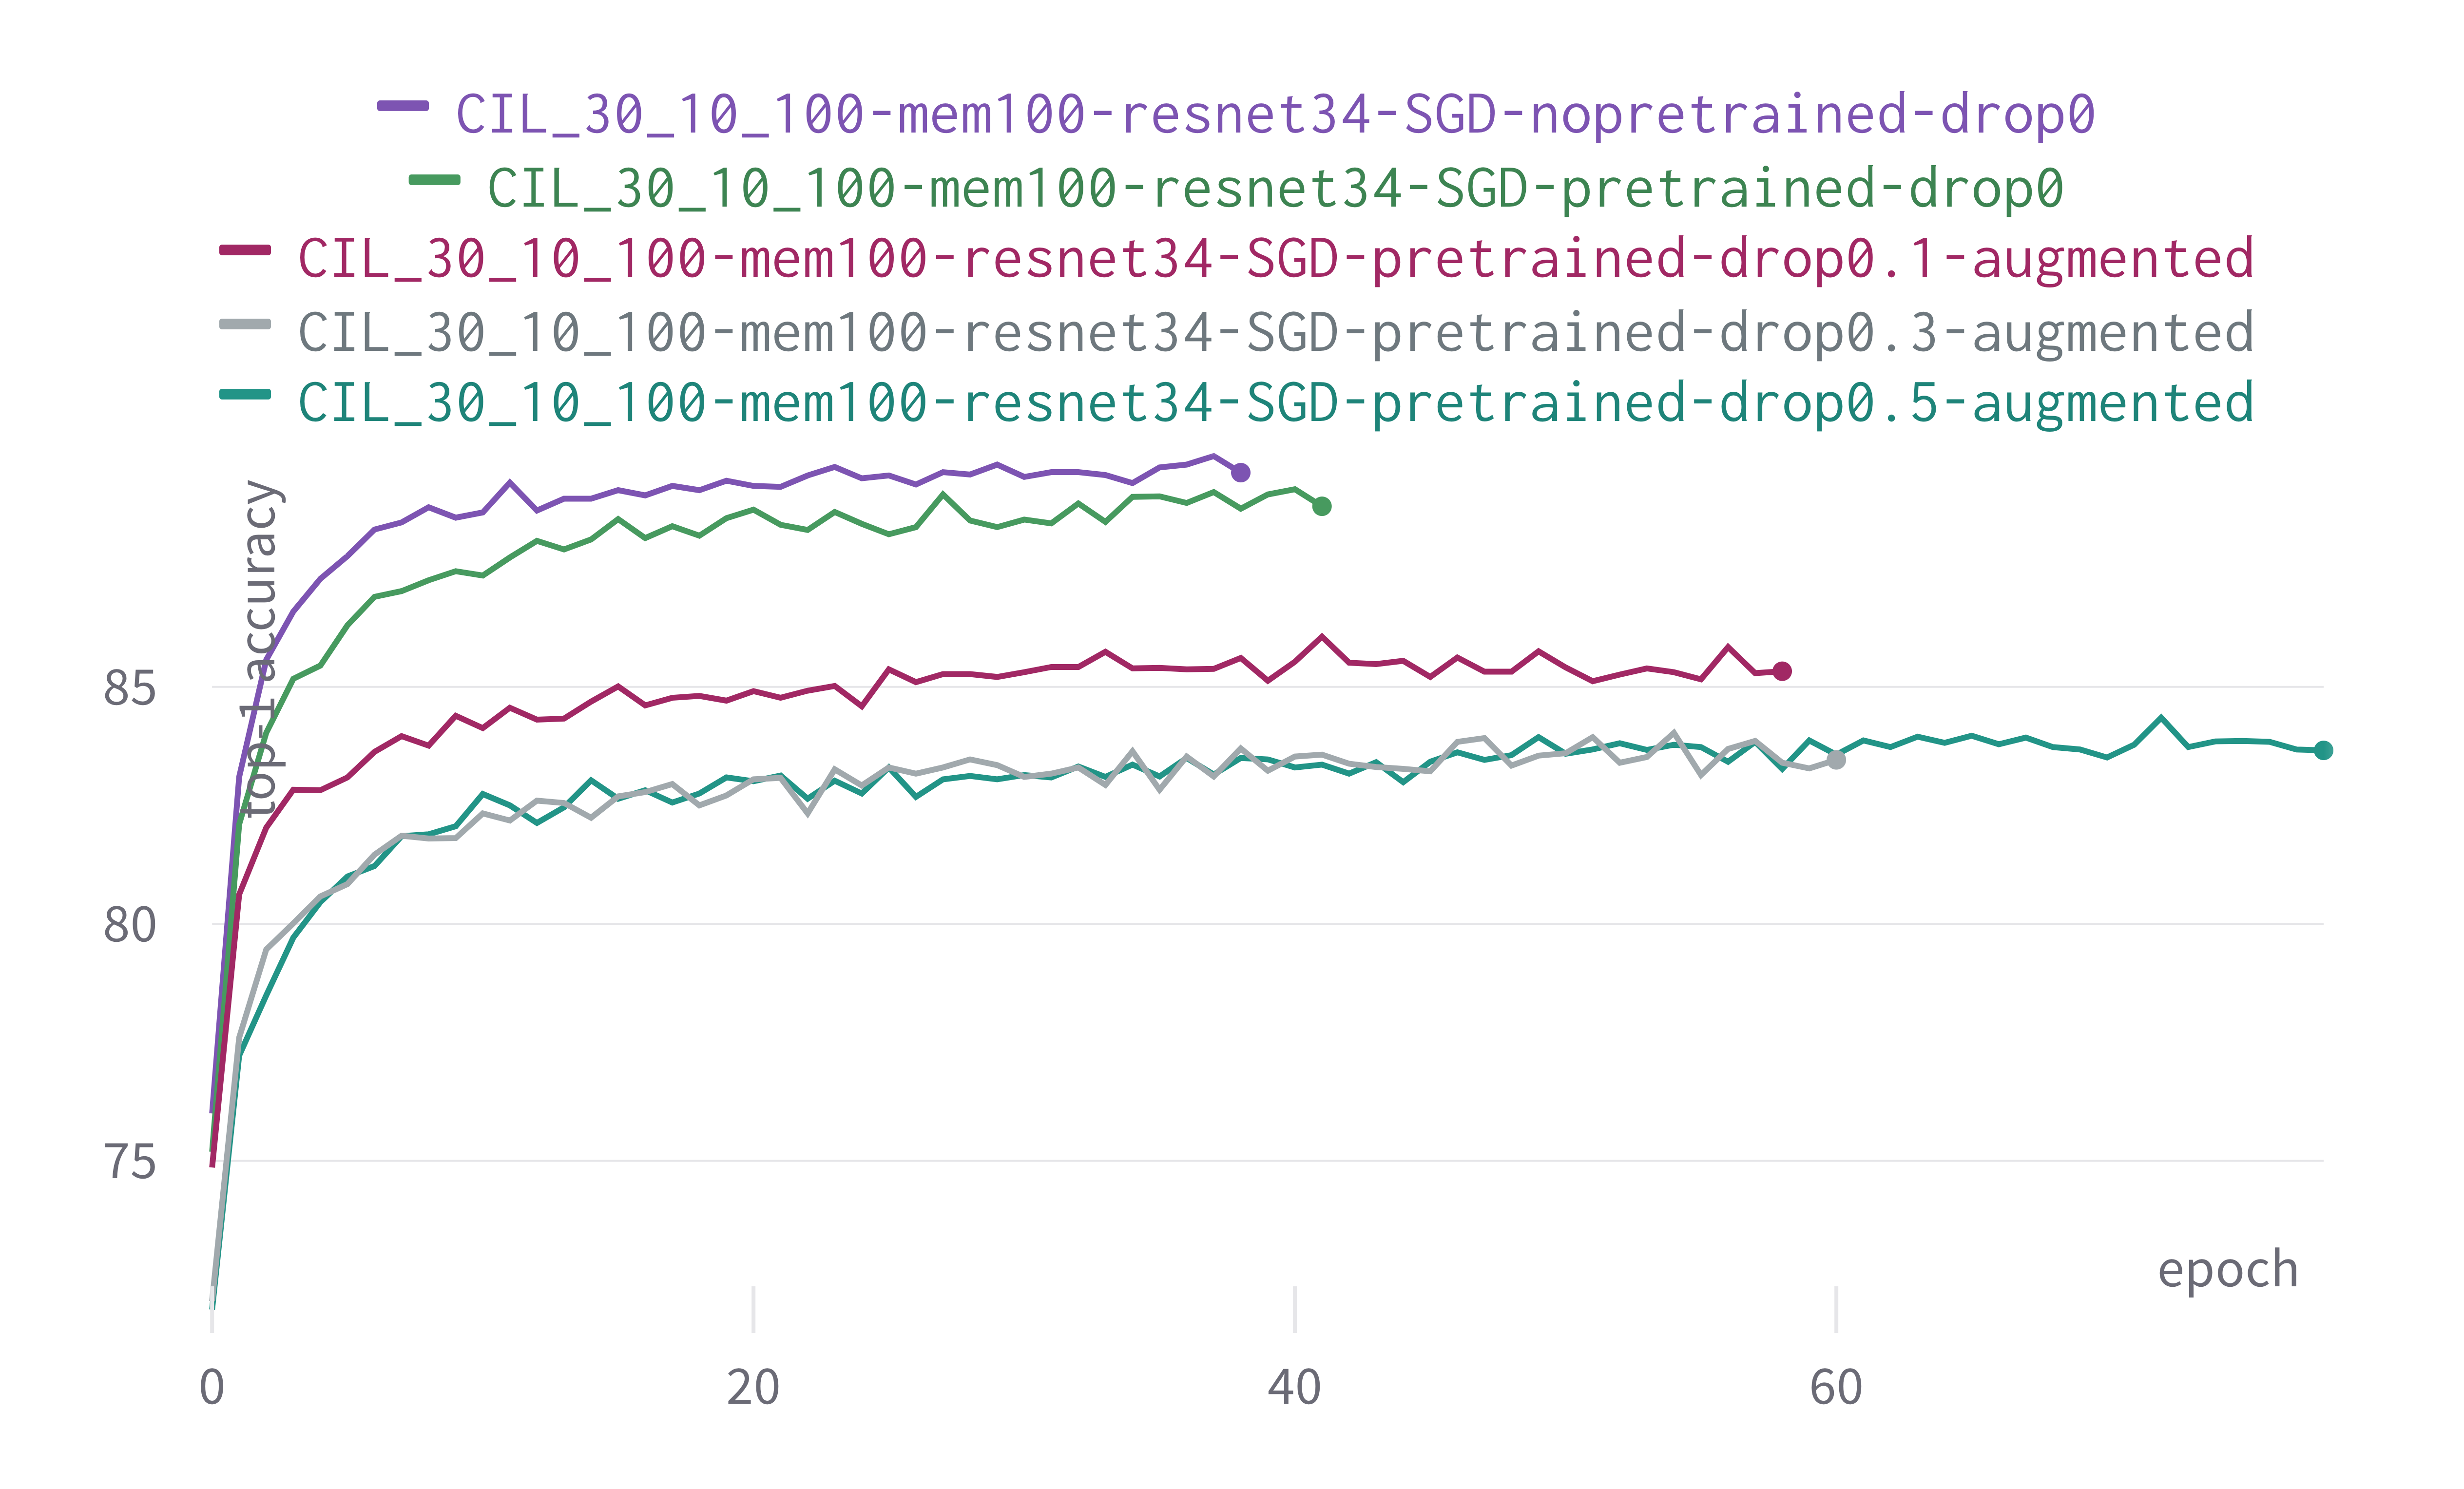
\includegraphics[width=0.80\textwidth]{images/exp/exp2-train.png} }}%
    \qquad
	\subfloat[\centering Accuracy on the validation set]{{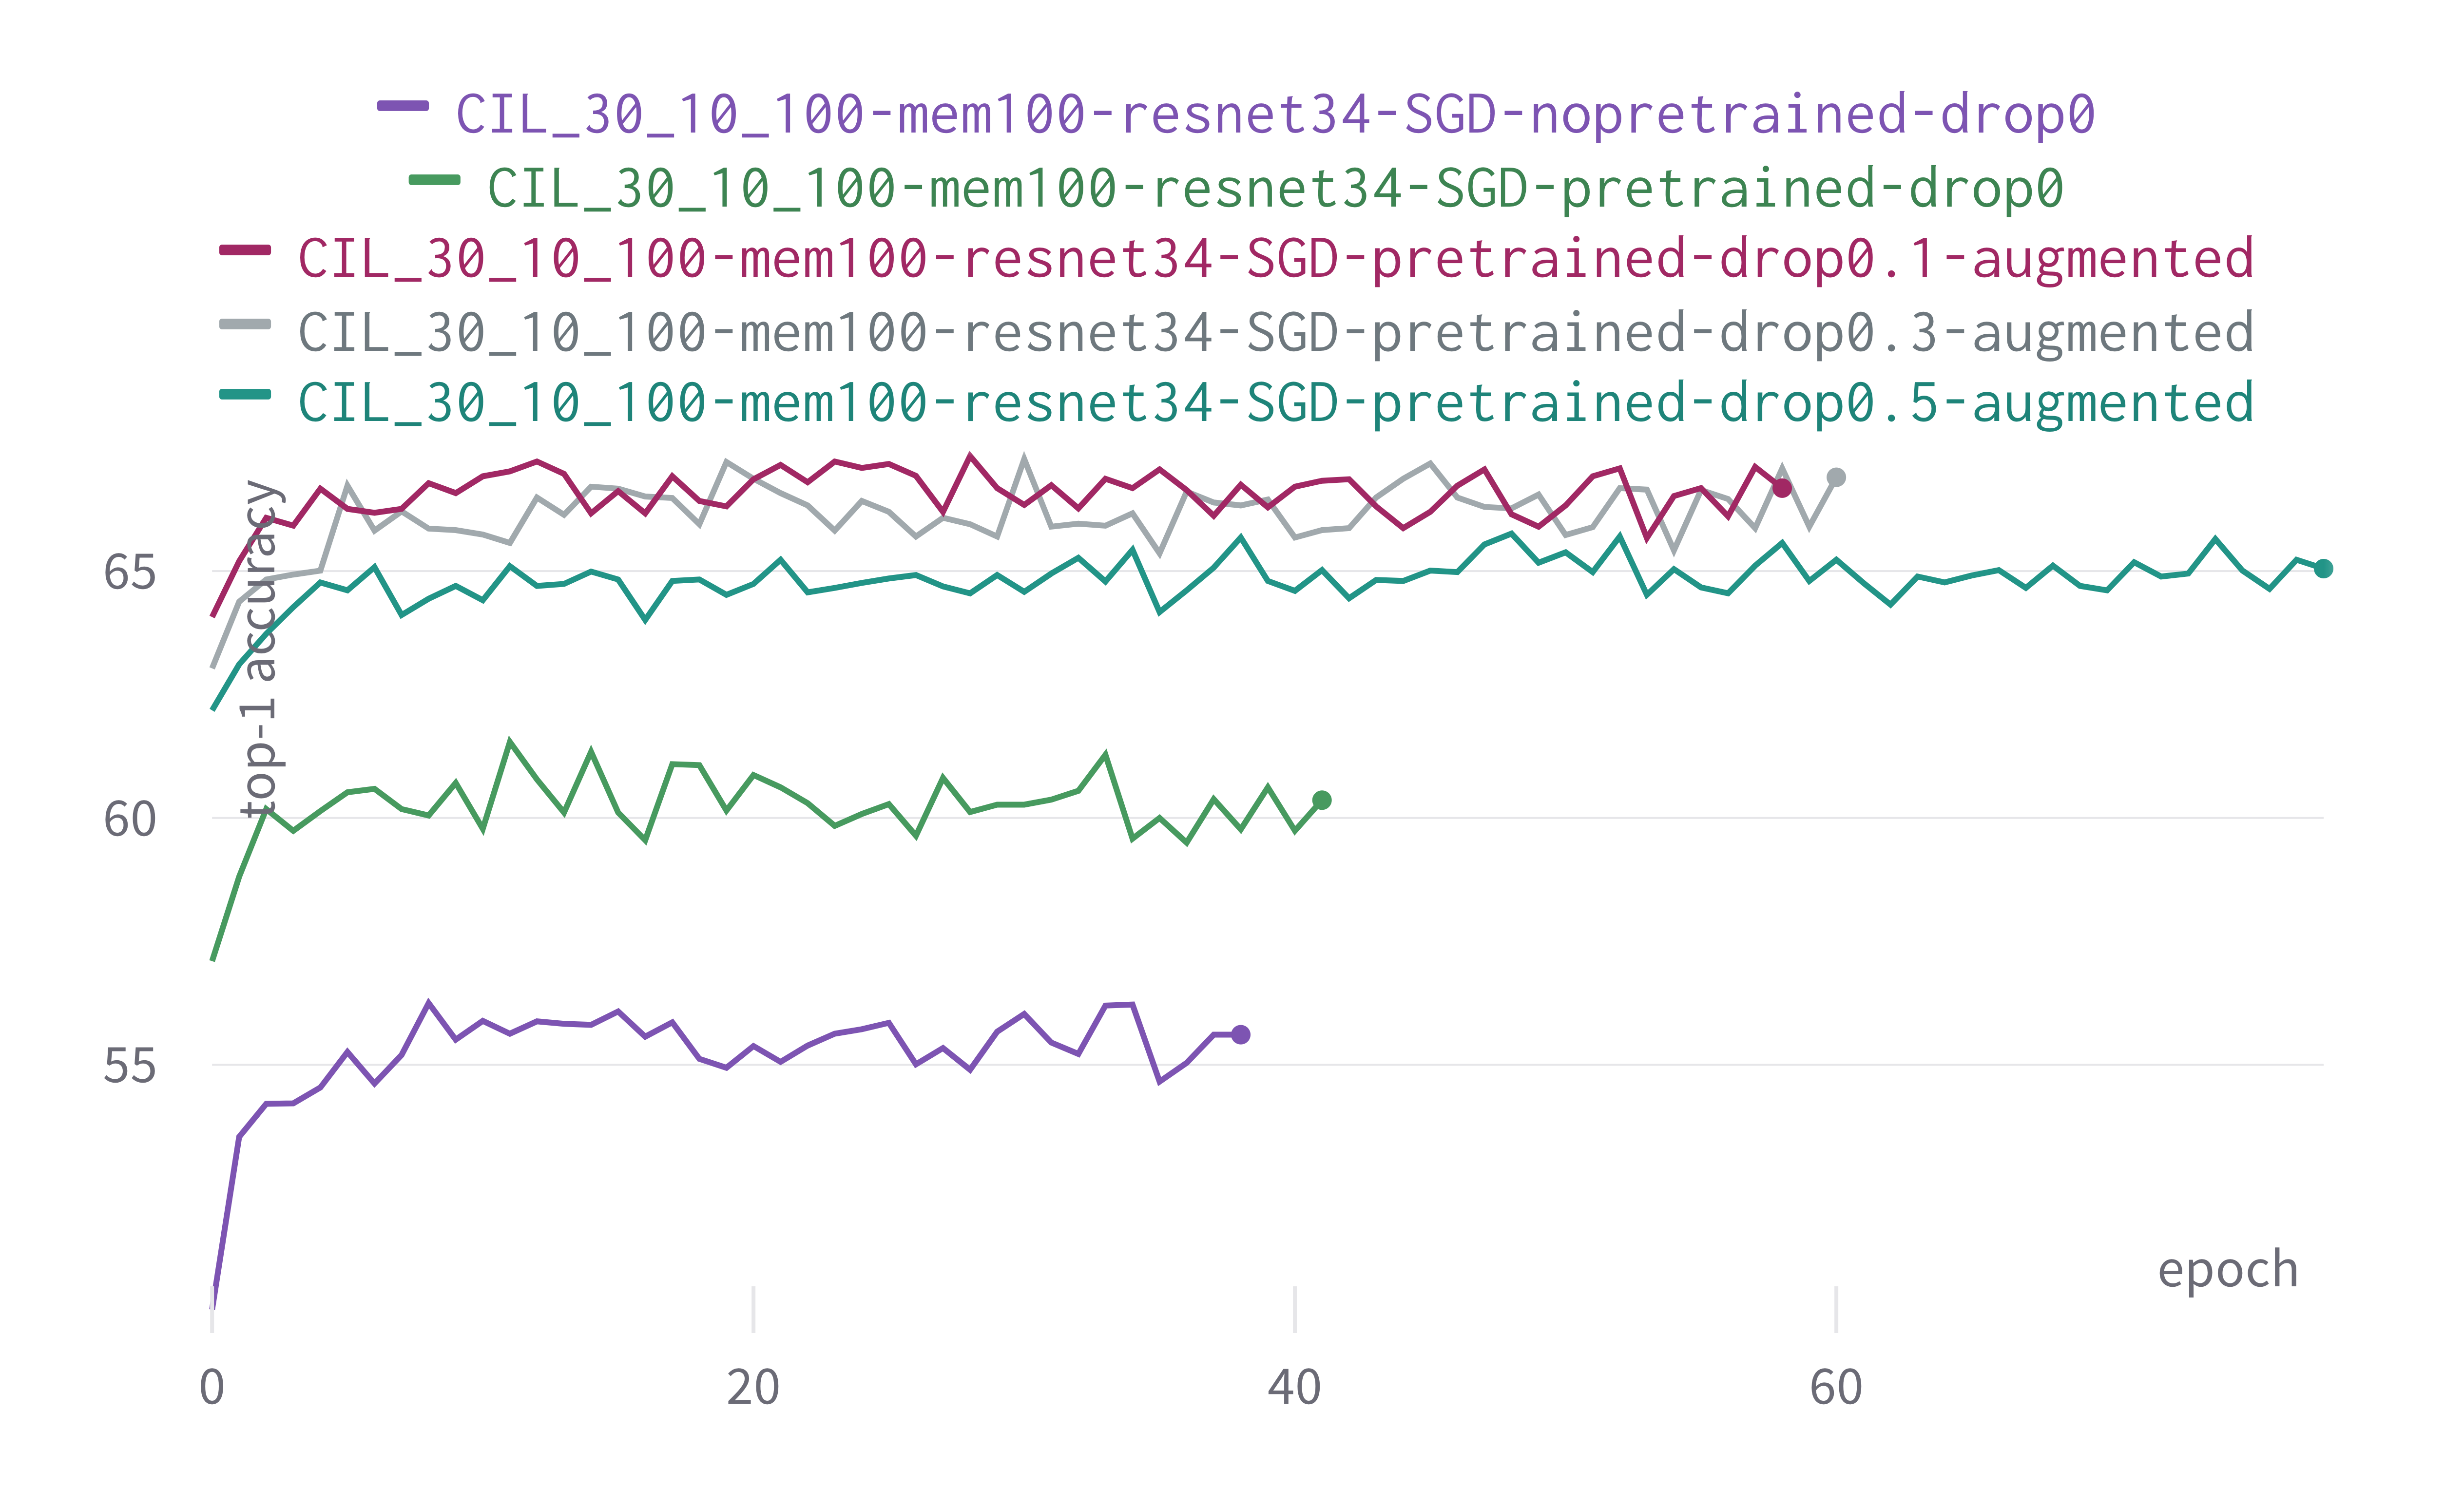
\includegraphics[width=0.80\textwidth]{images/exp/exp2-val.png} }}%
	\caption{Regularized models with data augmentation: comparison of the top-1 accuracy at each training epoch at task 7 between training and validation.}%
	\label{fig:exp2-train_val}%
\end{figure}

\newpage
\subsubsection{Type 1 baseline}
To compare the performance of the CIL model with a standard non-incremental learning setup, a baseline is trained using the same train/validation/test split of the CIL model. In particular, this experiment exploits the definition of 'type 1 baseline' described in \autoref{sec:method-baseline1}, i.e. it uses the DER algorithm and trains the model at task 0 with all 100 classes. Analogous to the CIL model, the baseline uses data augmentation, the SGD optimizer, a dropout layer before the FC layer and ResNet-34 pre-trained on ImageNet as backbone for the feature extract.

The performance comparison between the CIL models and the baselines is compared considering the top-1 accuracy on the test set. The results are shown in \autoref{table:baseline1}. As we can see, the best CIL model performs better than the best baseline, which is the opposite of what one might expect. However, as we can see from \autoref{table:baseline1-params}, this is due to the difference in the number of parameters described in \autoref{sec:method-baseline1}. For this reason, in the section section the CIL models are compared using a different type of baseline.

\begin{table}[H]
    \centering
    \centerline{
    \begin{tabular}{c|c|c}
        \hline
        \textbf{Model} &
        \textbf{Dropout} &
        \textbf{Top-1}\\
        \textbf{name} &
        \textbf{rate} &
        \textbf{acc. (\%)} \\
        \hline
\hline
SGD-pretrained-drop0.1-augmented&0.1&67.17\\
SGD-pretrained-drop0.3-augmented&0.3&\textbf{67.28}\\
SGD-pretrained-drop0.5-augmented&0.5&65.57\\
\hline
BASELINE\_1-pretrained-drop0.1-augmented&0.1&63.04\\
BASELINE\_1-pretrained-drop0.3-augmented&0.3&61.15\\
BASELINE\_1-pretrained-drop0.5-augmented&0.5&57.14\\
\hline 
    \end{tabular}}
    \caption{Performance comparison between the CIL model and the type 1 baseline. Top-1 accuracy at task 7 (CIL model) and task 0 (baseline).}
    \label{table:baseline1}
\end{table}

\begin{table}[H]
    \centering
    \centerline{
    \begin{tabular}{c|c}
        \hline
        \textbf{Model} &
        \textbf{\#Params} \\
        \textbf{name} &
        \textbf{(M)} \\
        \hline
\hline
SGD-pretrained-drop0.1-augmented&170\\
SGD-pretrained-drop0.3-augmented&170\\
SGD-pretrained-drop0.5-augmented&170\\
\hline
BASELINE\_1-pretrained-drop0.1-augmented&21\\
BASELINE\_1-pretrained-drop0.3-augmented&21\\
BASELINE\_1-pretrained-drop0.5-augmented&21\\
\hline 
    \end{tabular}}
    \caption{Number of model parameters between the CIL model and the typ 1 baseline. Number of parameters at task 7 (CIL model) and task 0 (baseline).}
    \label{table:baseline1-params}
\end{table}

\subsubsection{Top-100 Classes}
\label{sec:cil-top100}
In order to assess the extent to which those classes with few examples contribute to performance deterioration, the next experiments are carried out by considering only the top-100 classes, i.e. those with the largest number of examples (see the left-hand side of the distribution in \autoref{fig:logodet-dist}). This is useful to be aware of how much the model is limited in performance by the dataset.

Considering the regularized models and data augmentation, models trained on 100 randomly sampled classes and those trained on the top-100 classes are compared in \autoref{fig:exp3} and \autoref{table:exp3}. As we can see, even if the top-5 accuracy does not change between the two cases, considering the top-1 accuracy there is a drastic improvement in performance. This is a clear sign that classes with few examples deteriorate performance a lot.

\begin{table}[H]
    \centering
    \centerline{
    \begin{tabular}{c|c|c|c|c}
        \hline
        \textbf{Model} &
        \textbf{Dropout} &
        \textbf{Sampling} &
        \textbf{Top-1} & 
        \textbf{Top-5} \\
        \textbf{name} &
        \textbf{rate} &
        \textbf{method} &
        \textbf{acc. (\%)} & 
        \textbf{acc. (\%)} \\
        \hline
        \hline
drop0.1-augmented&0.1&random&	67.17&98.15\\
drop0.3-augmented&0.3&random&67.28&	97.3\\
drop0.5-augmented&0.5&random&65.57&	96.24\\
\hline
drop0.1-augmented-onlytop&0.1&top-100&\textbf{89.1}&\textbf{96.59}\\
drop0.3-augmented-onlytop&0.3&top-100&88.14&96.39\\
drop0.5-augmented-onlytop&0.5&top-100&87.6&95.92\\
        \hline
    \end{tabular}}
    \caption{Comparison of models trained on 100 randomly sampled classed and top-100 classes. Top-1 accuracy at task 7.}
    \label{table:exp3}
\end{table}
\newpage
\begin{figure}[H]
	\centering
	\subfloat[\centering Top-1 accuracy]{{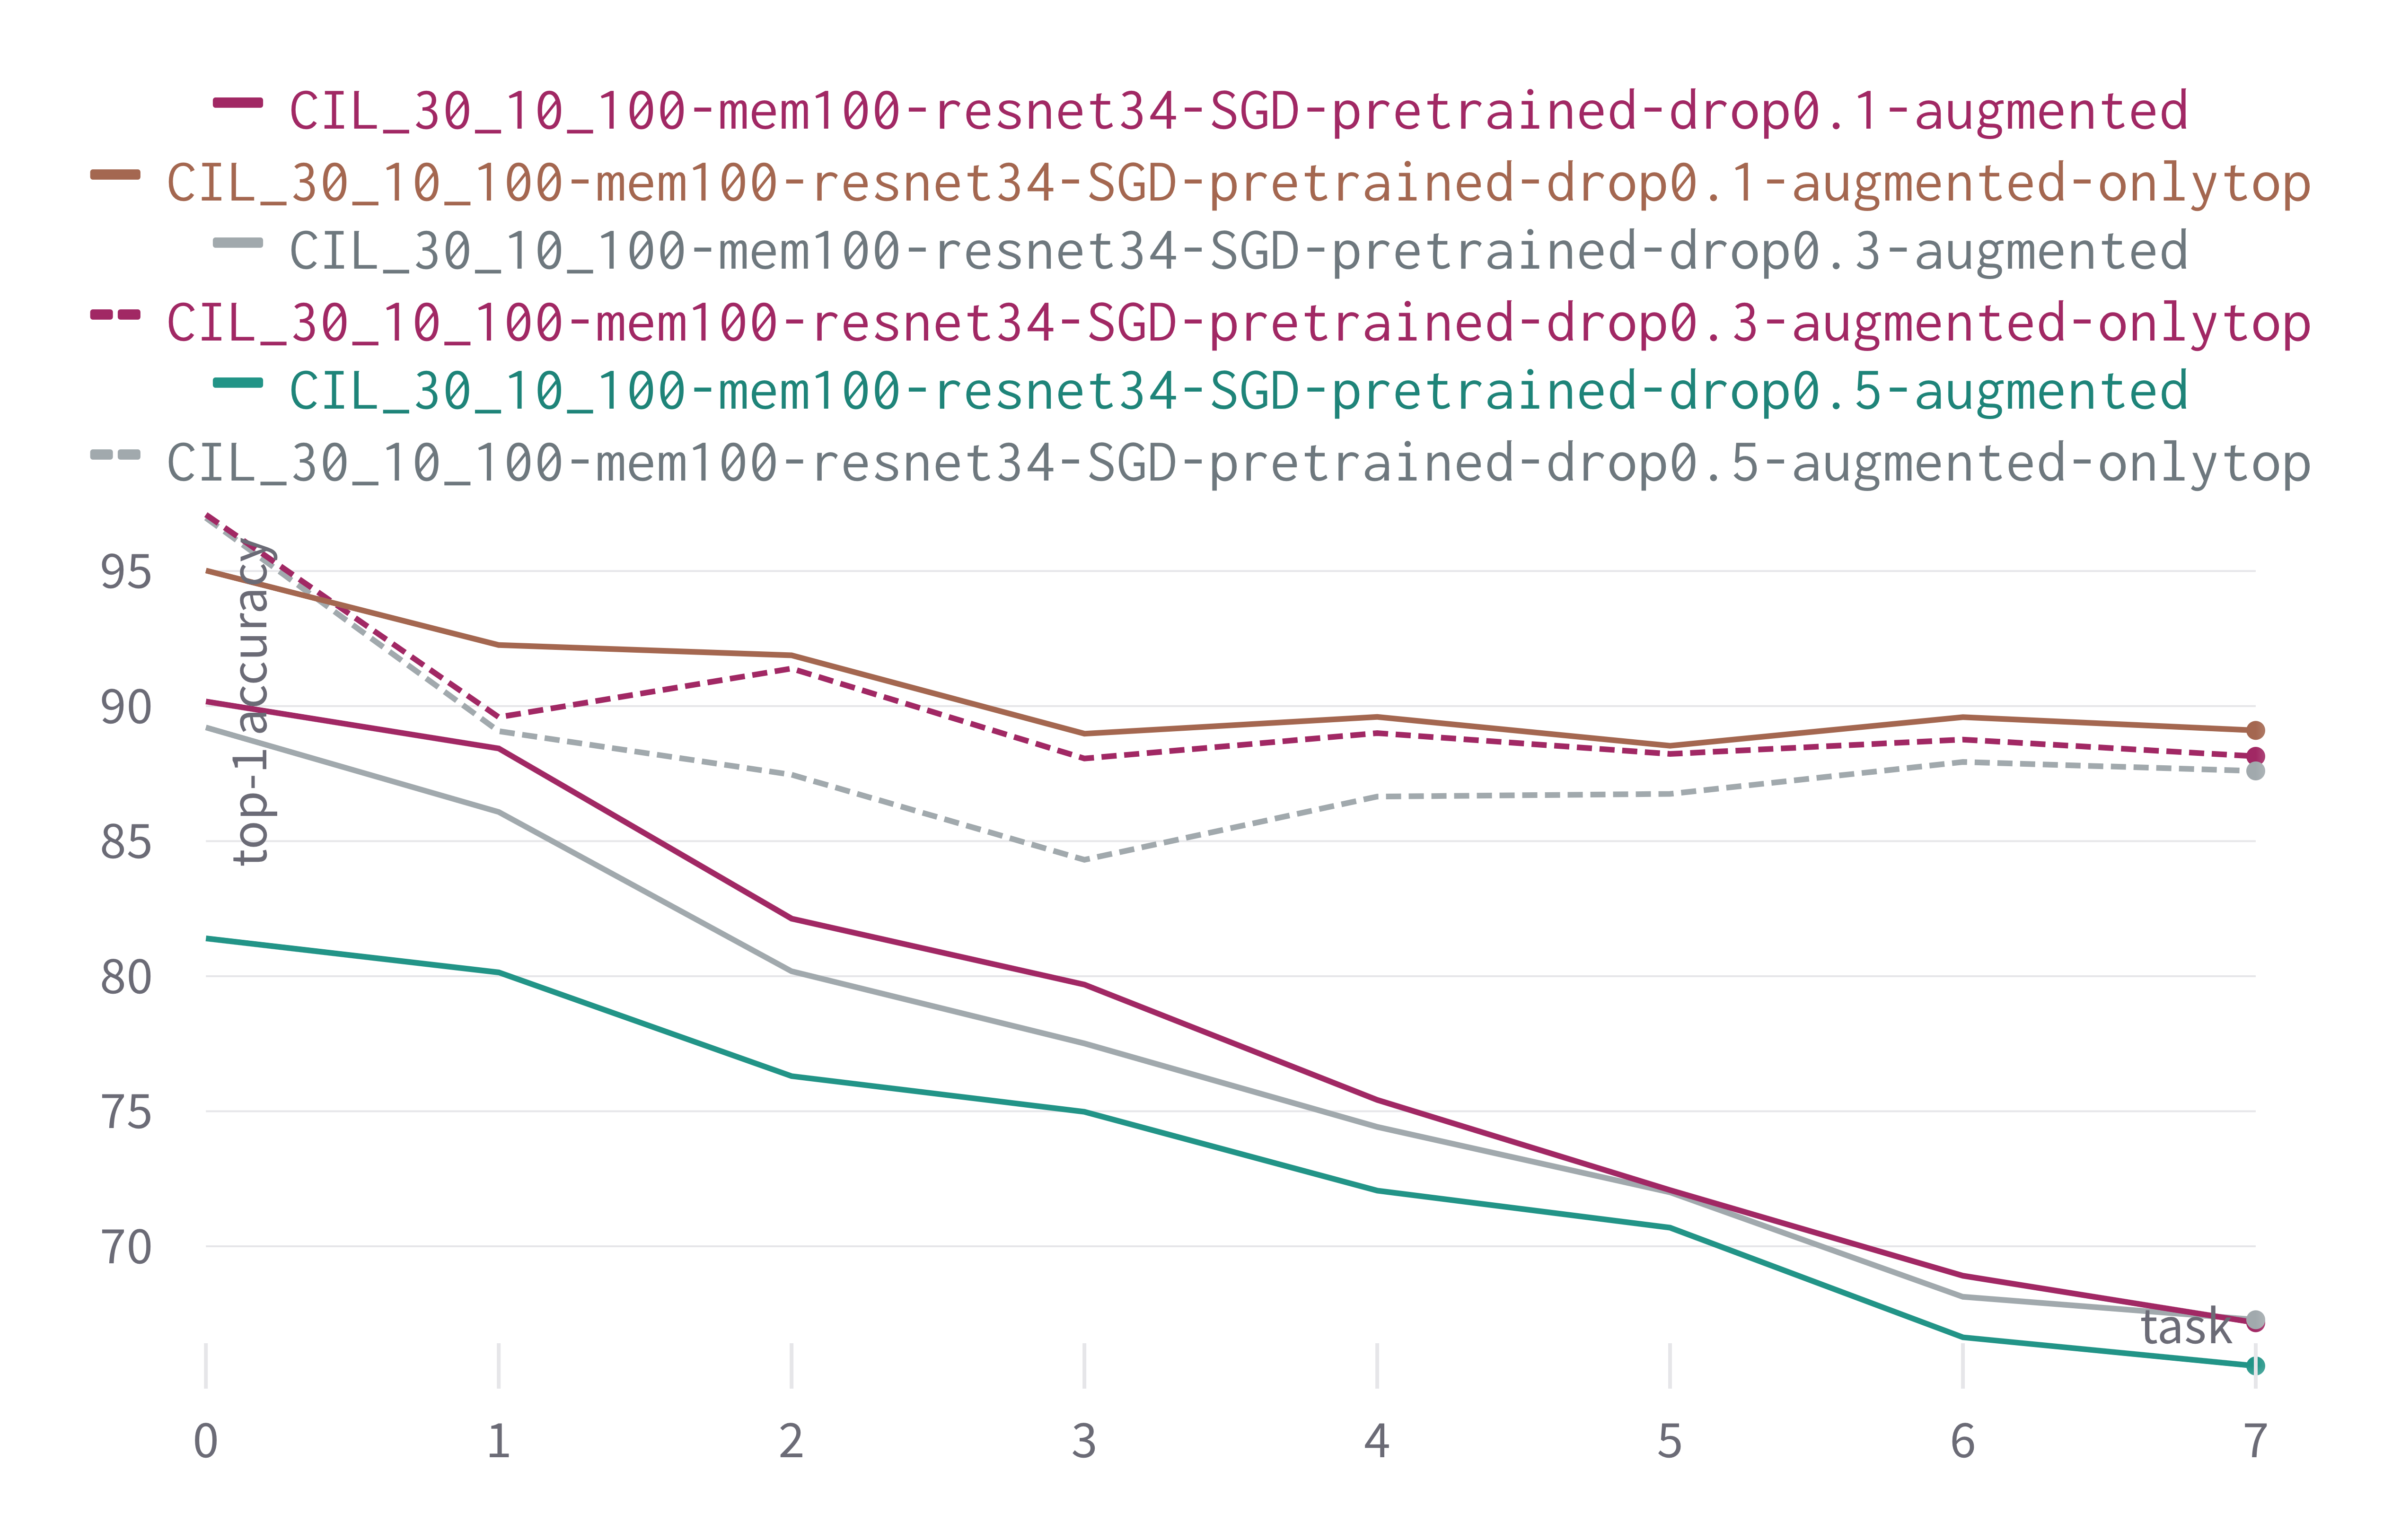
\includegraphics[width=0.80\textwidth]{images/exp/exp3-top1.png} }}%
    \qquad
	\subfloat[\centering Top-5 accuracy]{{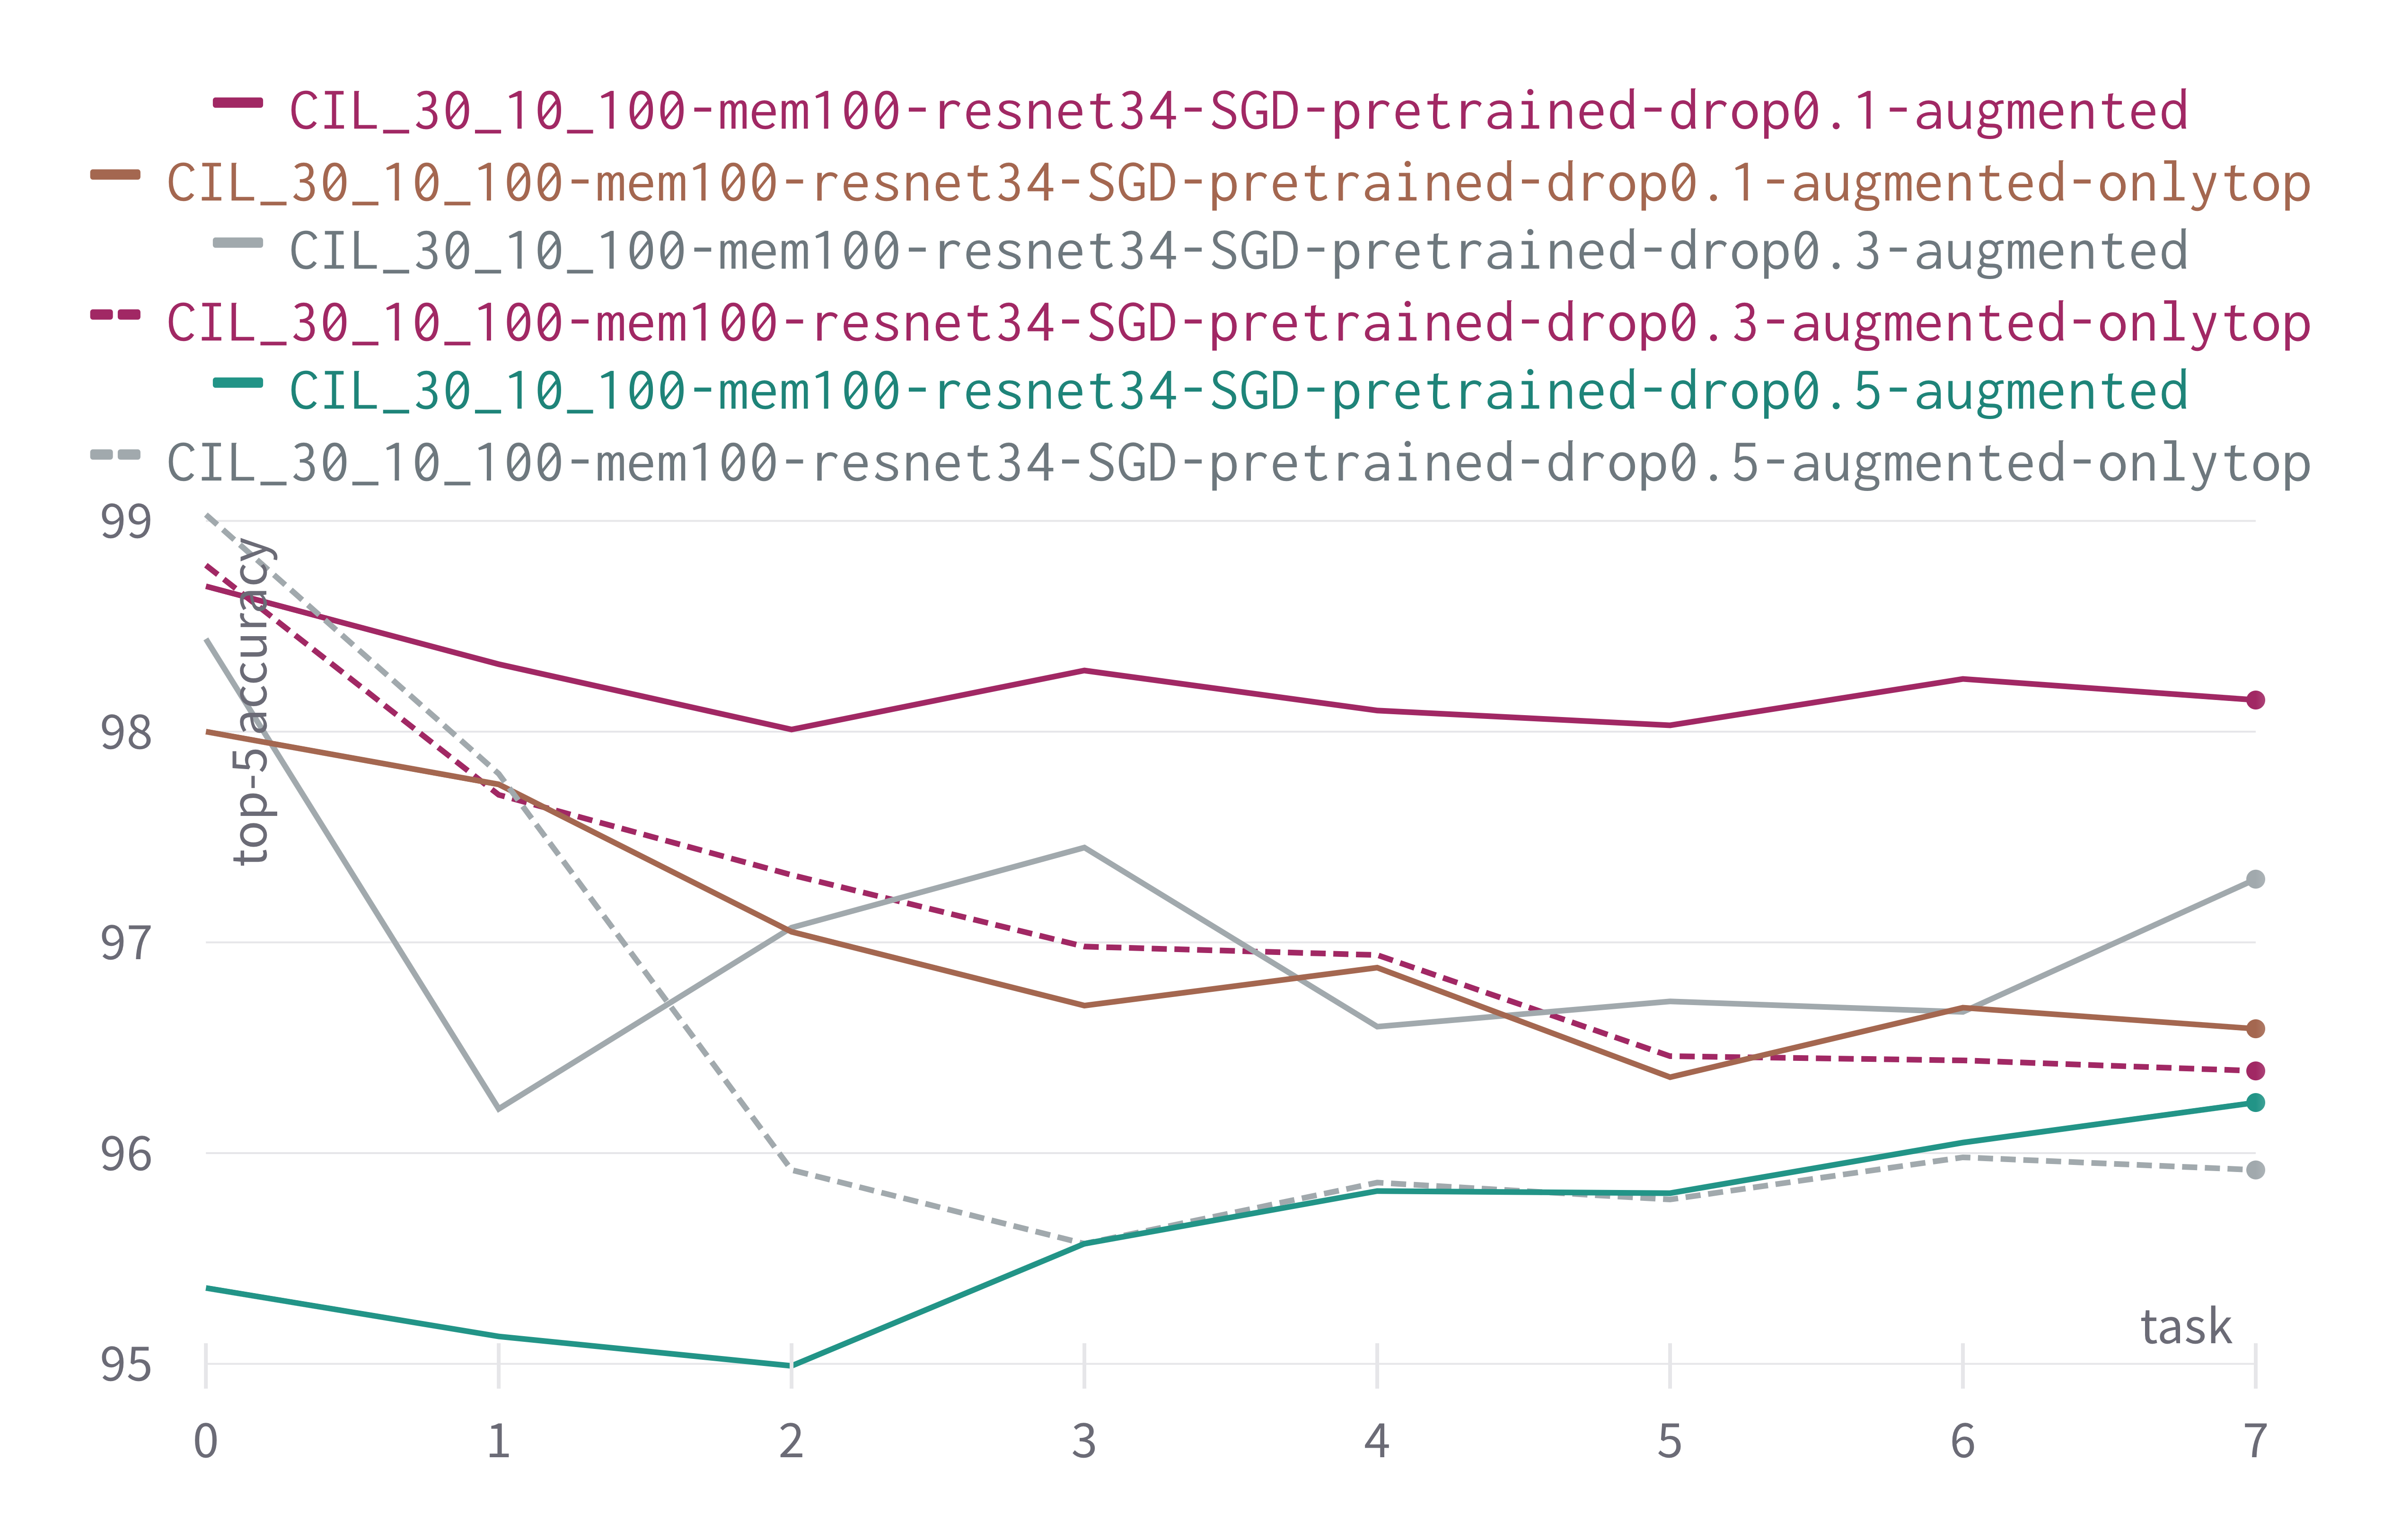
\includegraphics[width=0.80\textwidth]{images/exp/exp3-top5.png} }}%
	\caption{Comparison of models trained on 100 randomly sampled classed and top-100 classes.}%
	\label{fig:exp3}%
\end{figure}

\newpage
\subsubsection{Introduction of Adam optimizer}
The next experiments aim to compare the SGD (see \autoref{sec:sgd_opt}) and Adam (see \autoref{sec:adam_opt}) optimizers. Considering the regularized models, data augmentation and the top-100 classes, the result of this comparison is shown in \autoref{fig:exp4} and \autoref{table:exp4}.


As we can see from the results shown in \autoref{table:exp4}, the top-1 accuracy at task 7 improves by more than 6\% using the Adam as the optimization algorithm. 
In addition to the performance aspect, the training history in \autoref{fig:exp4-train_val} shows that Adam leads to faster convergence. In fact the models trained with this algorithm achieve the highest value of top-1 accuracy on the validation set after only a few training epochs.

\begin{table}[H]
    \centering
    \centerline{
    \begin{tabular}{c|c|c|c|c}
        \hline
        \textbf{Model} &
        \textbf{Dropout} &
        \textbf{Optimizer} &
        \textbf{Top-1} & 
        \textbf{Top-5} \\
        \textbf{name} &
        \textbf{rate} &
        \textbf{method} &
        \textbf{acc. (\%)} & 
        \textbf{acc. (\%)} \\
        \hline
        \hline
SGD-drop0.1-augmented-onlytop&0.1&SGD&89.1&96.59\\
SGD-drop0.3-augmented-onlytop&0.3&SGD&88.14&96.39\\
SGD-drop0.5-augmented-onlytop&0.5&SGD&87.6&95.92\\
\hline
adam-drop0.1-augmented-onlytop&0.1&Adam&92.15&97.92\\
adam-drop0.3-augmented-onlytop&0.3&Adam&91.55&97.75\\
adam-drop0.5-augmented-onlytop&0.5&Adam&\textbf{95.04}&\textbf{98.4}\\
        \hline
    \end{tabular}}
    \caption{Comparison of models trained using SGD and Adam. Top-1 accuracy at task 7.}
    \label{table:exp4}
\end{table}

\newpage

\begin{figure}[H]
	\centering
	\subfloat[\centering Top-1 accuracy]{{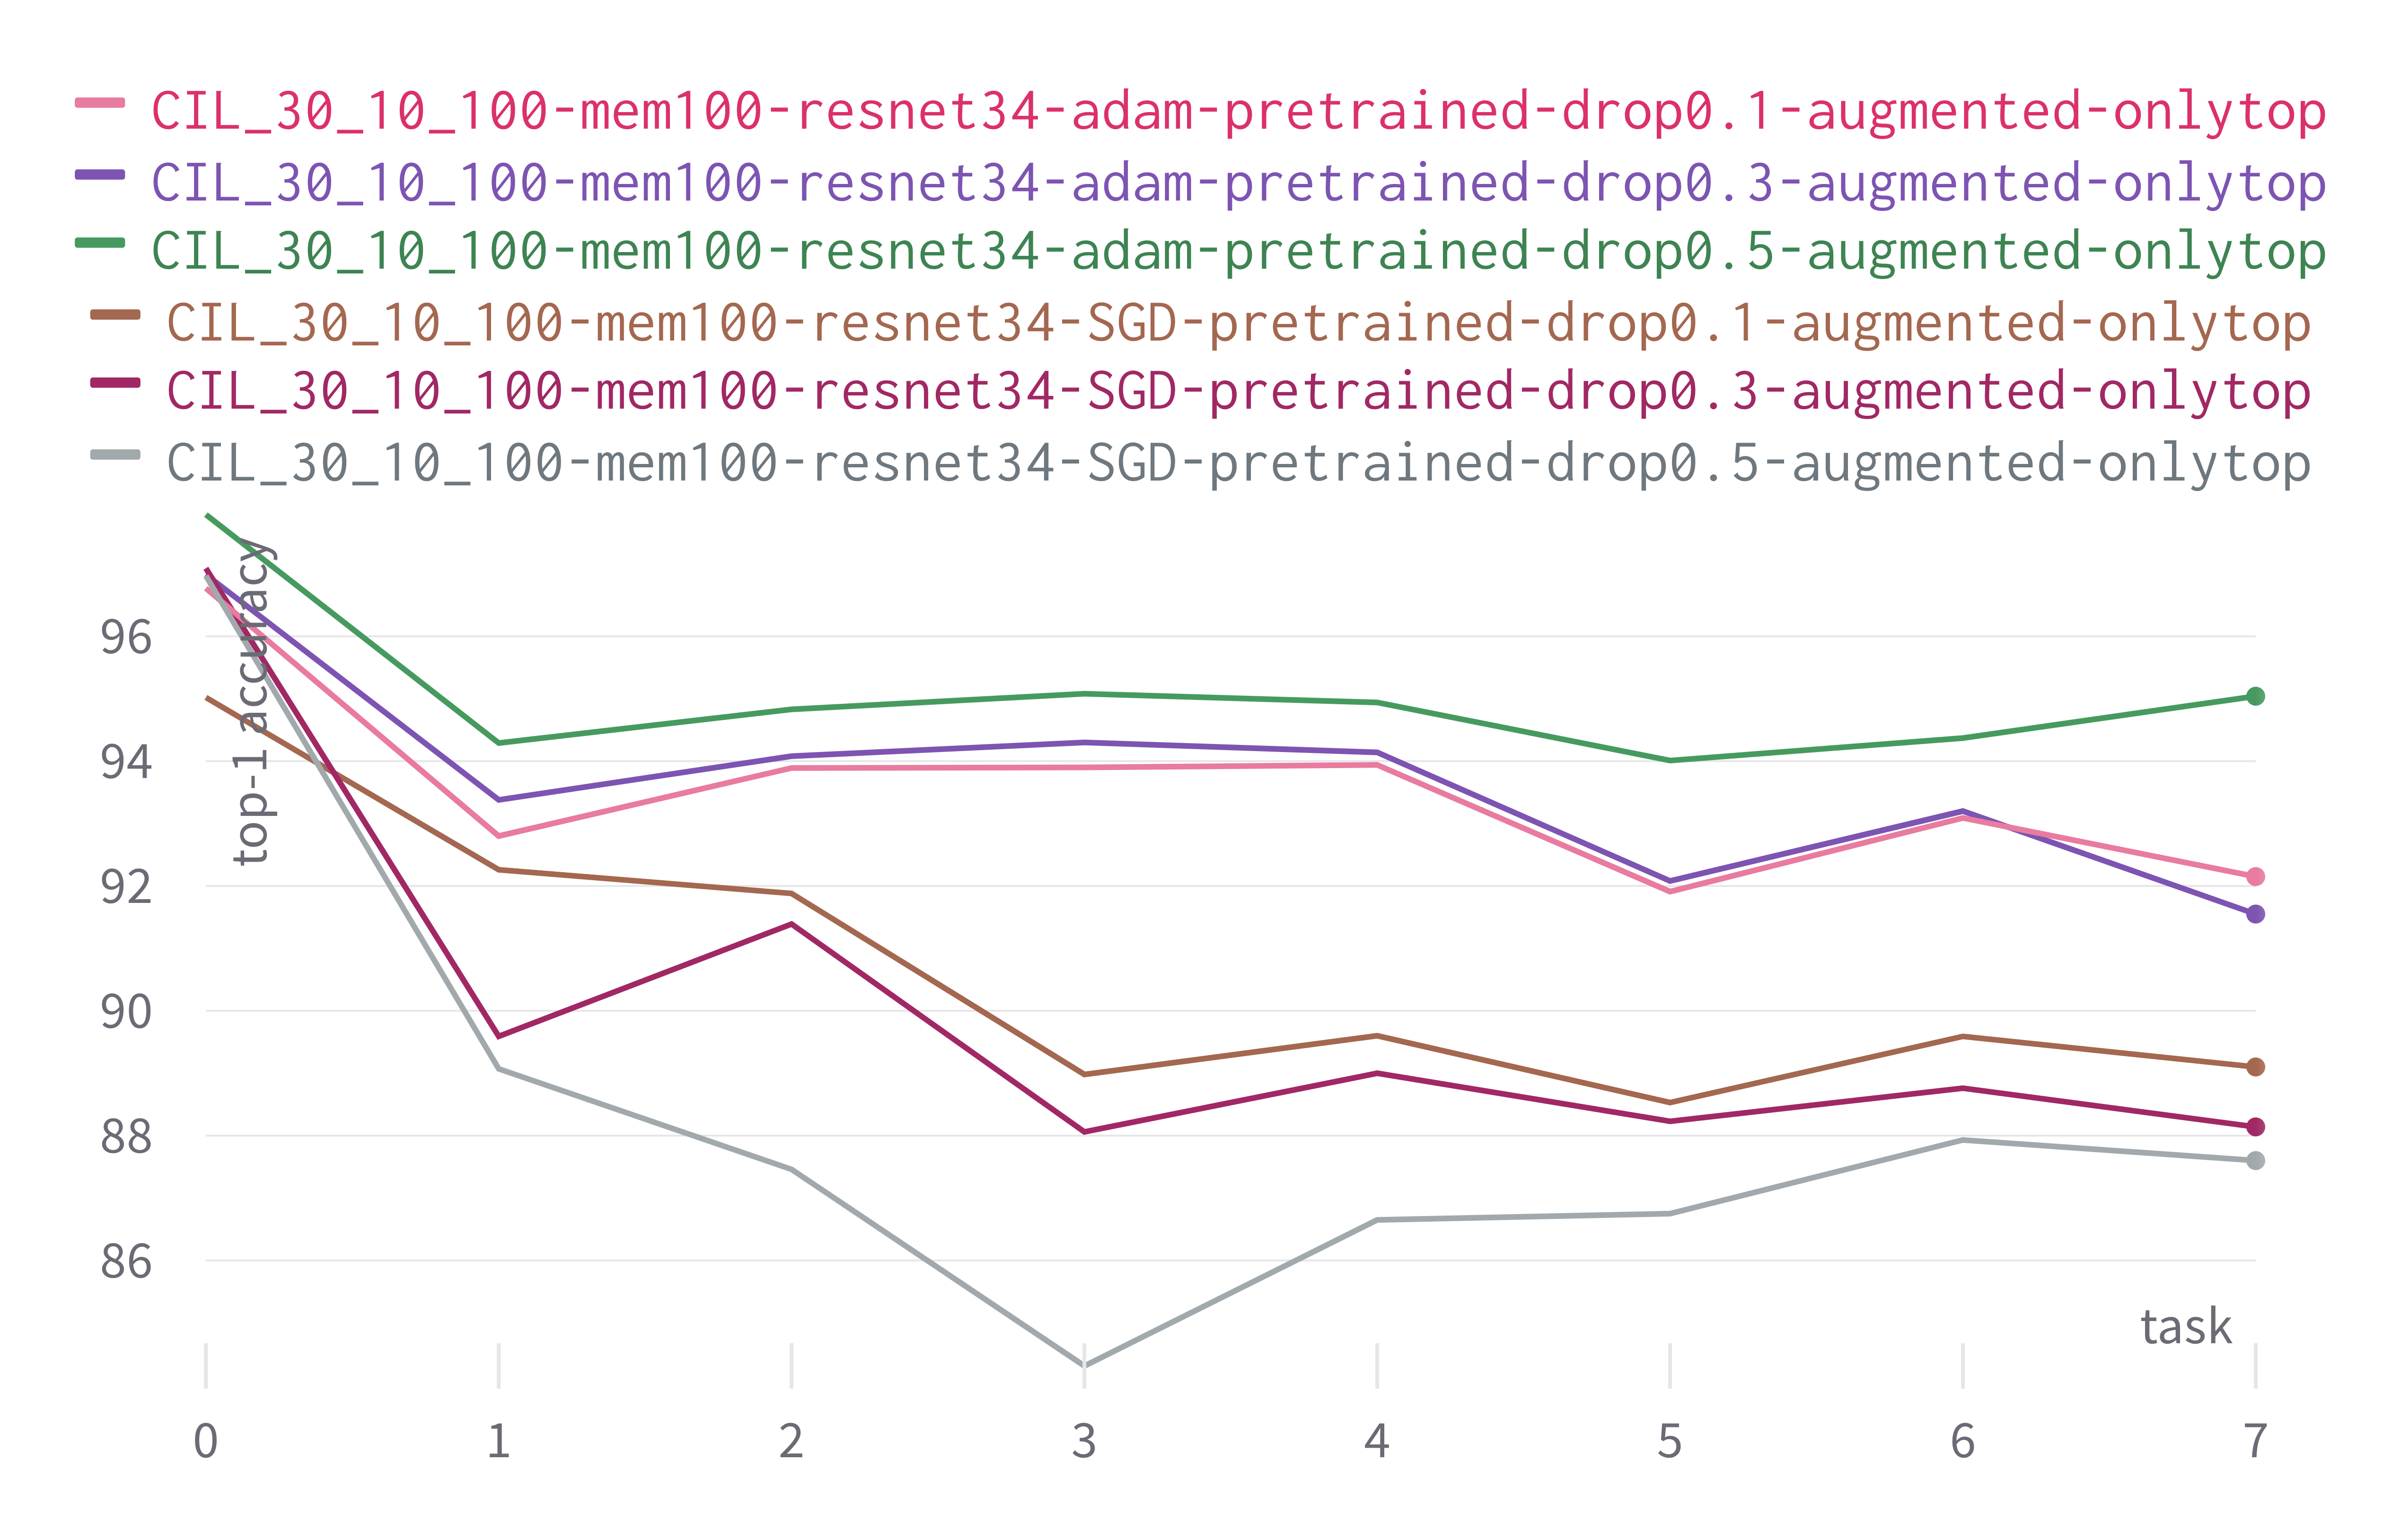
\includegraphics[width=0.80\textwidth]{images/exp/exp4-top1.png} }}%
    \qquad
	\subfloat[\centering Top-5 accuracy]{{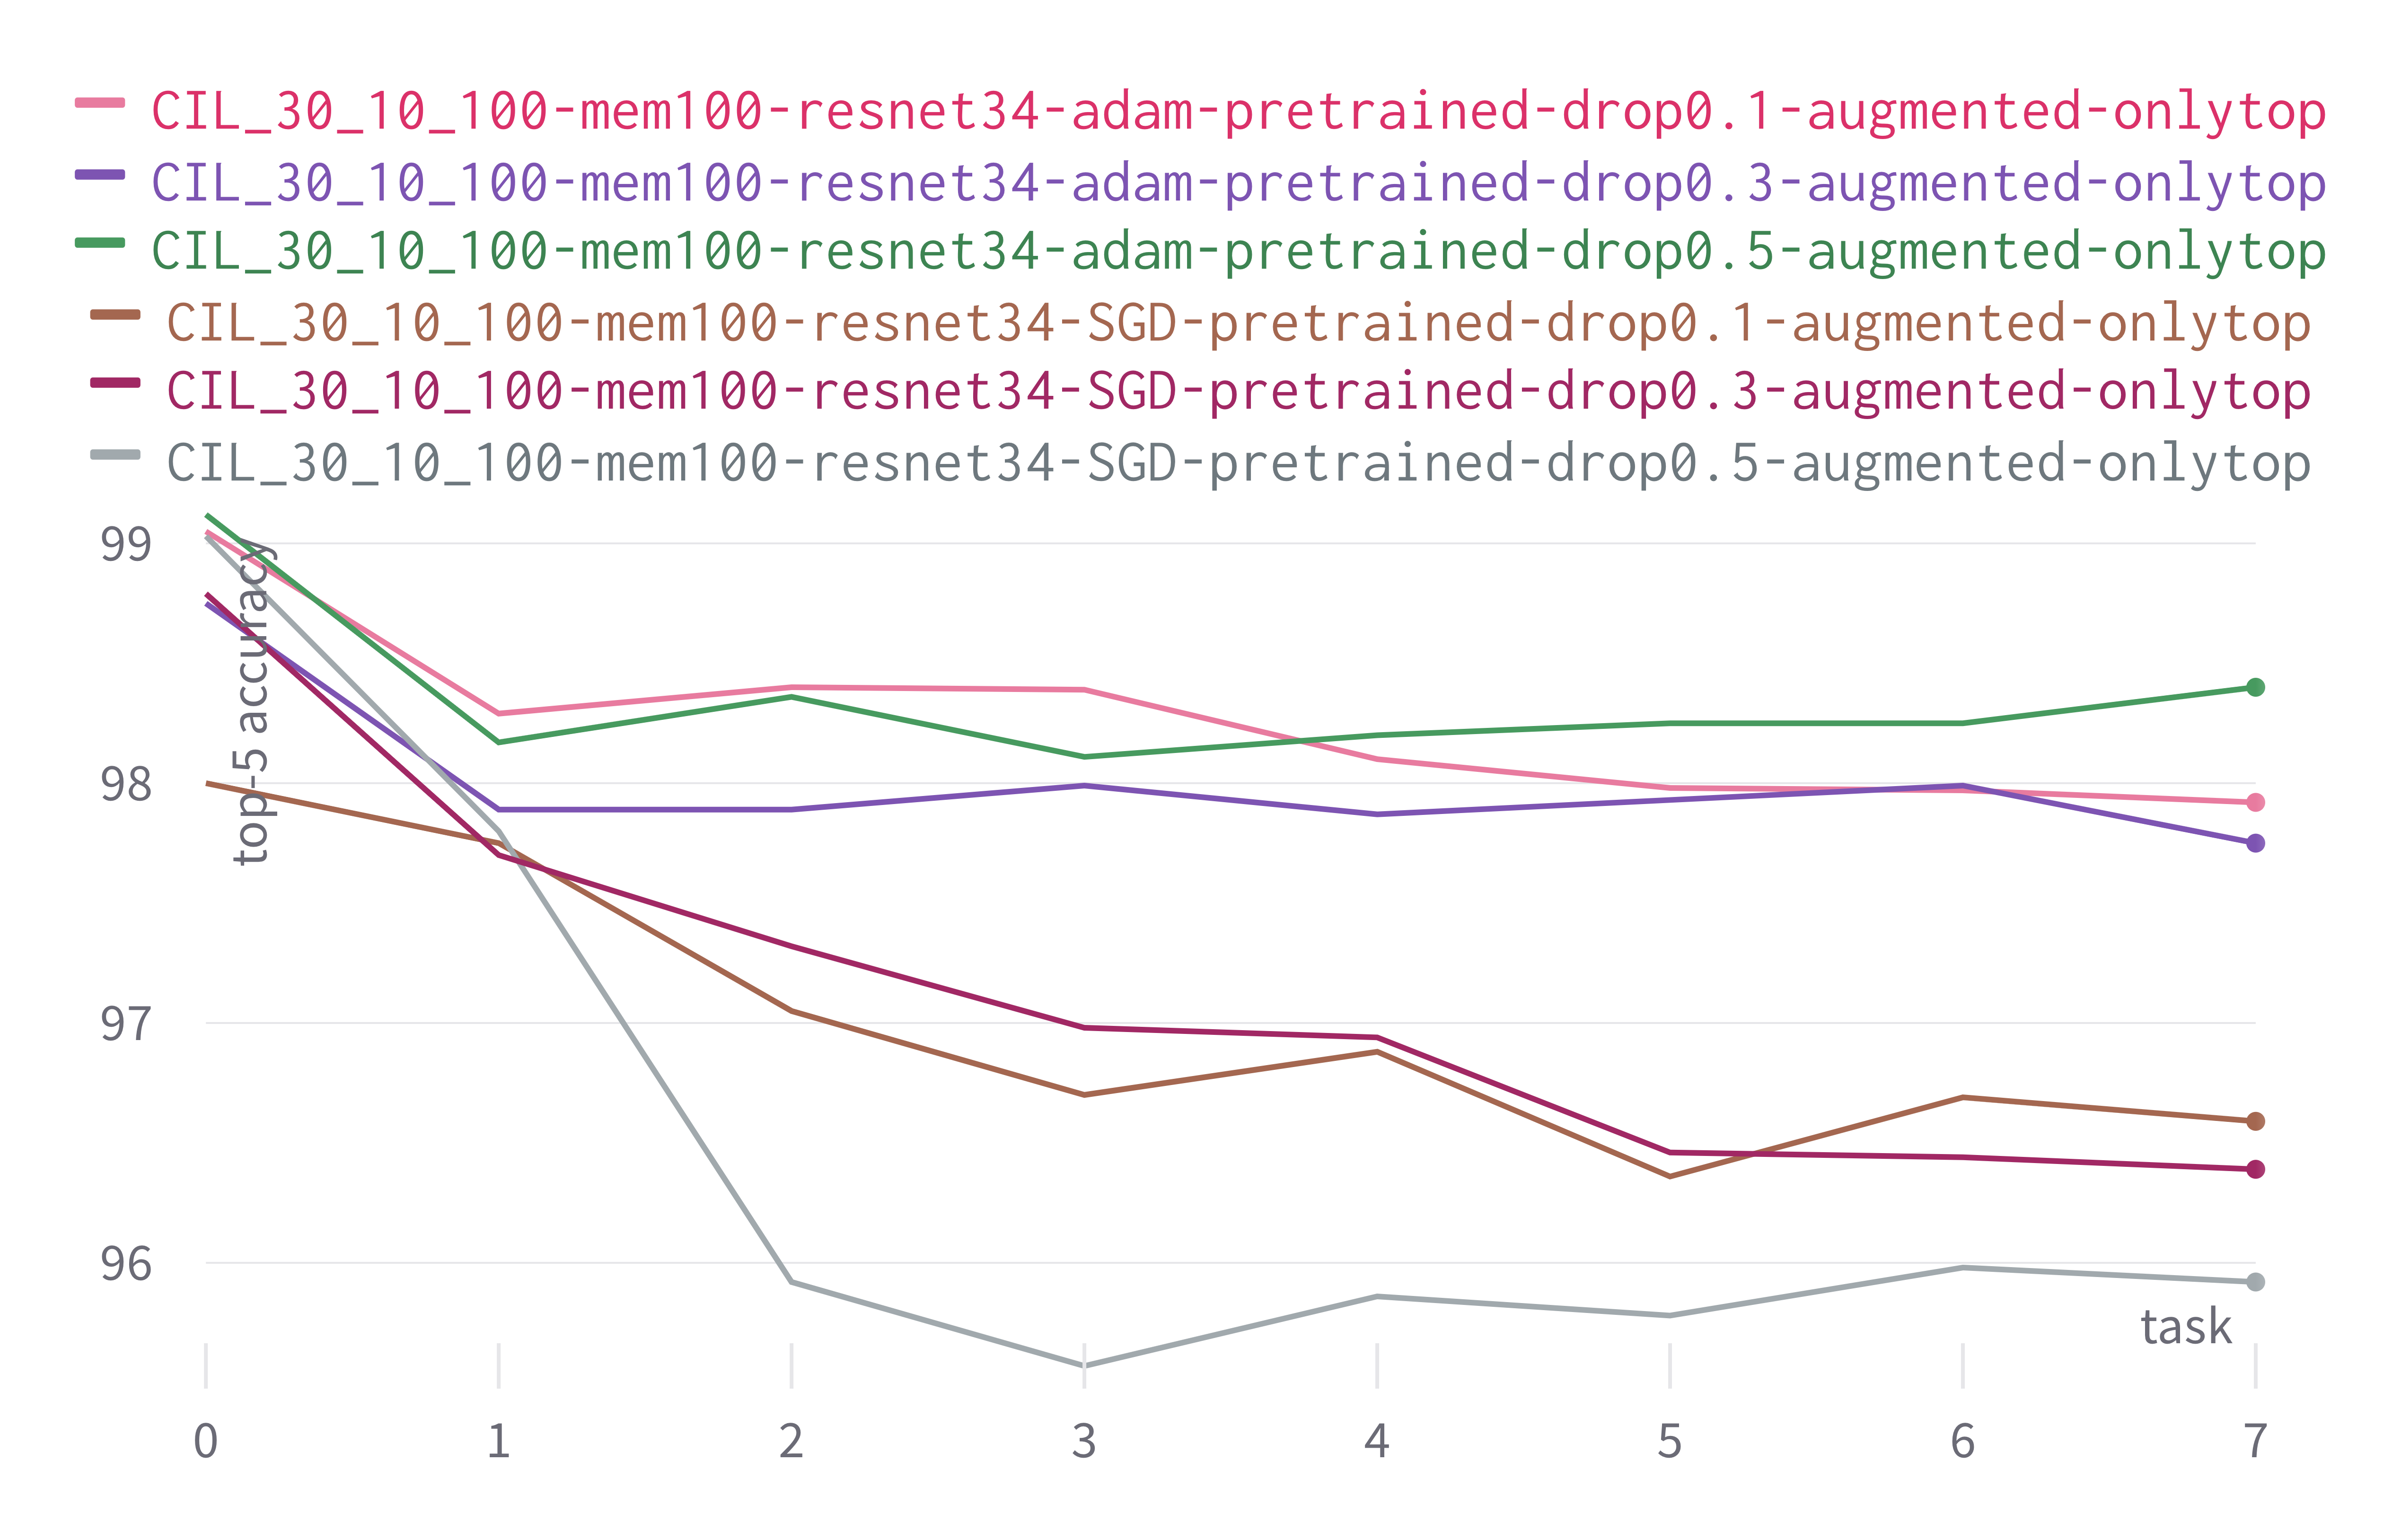
\includegraphics[width=0.80\textwidth]{images/exp/exp4-top5.png} }}%
	\caption{Comparison of models trained using SGD and Adam.}%
	\label{fig:exp4}%
\end{figure}

\begin{figure}[H]
	\centering
	\subfloat[\centering Accuracy on the training set]{{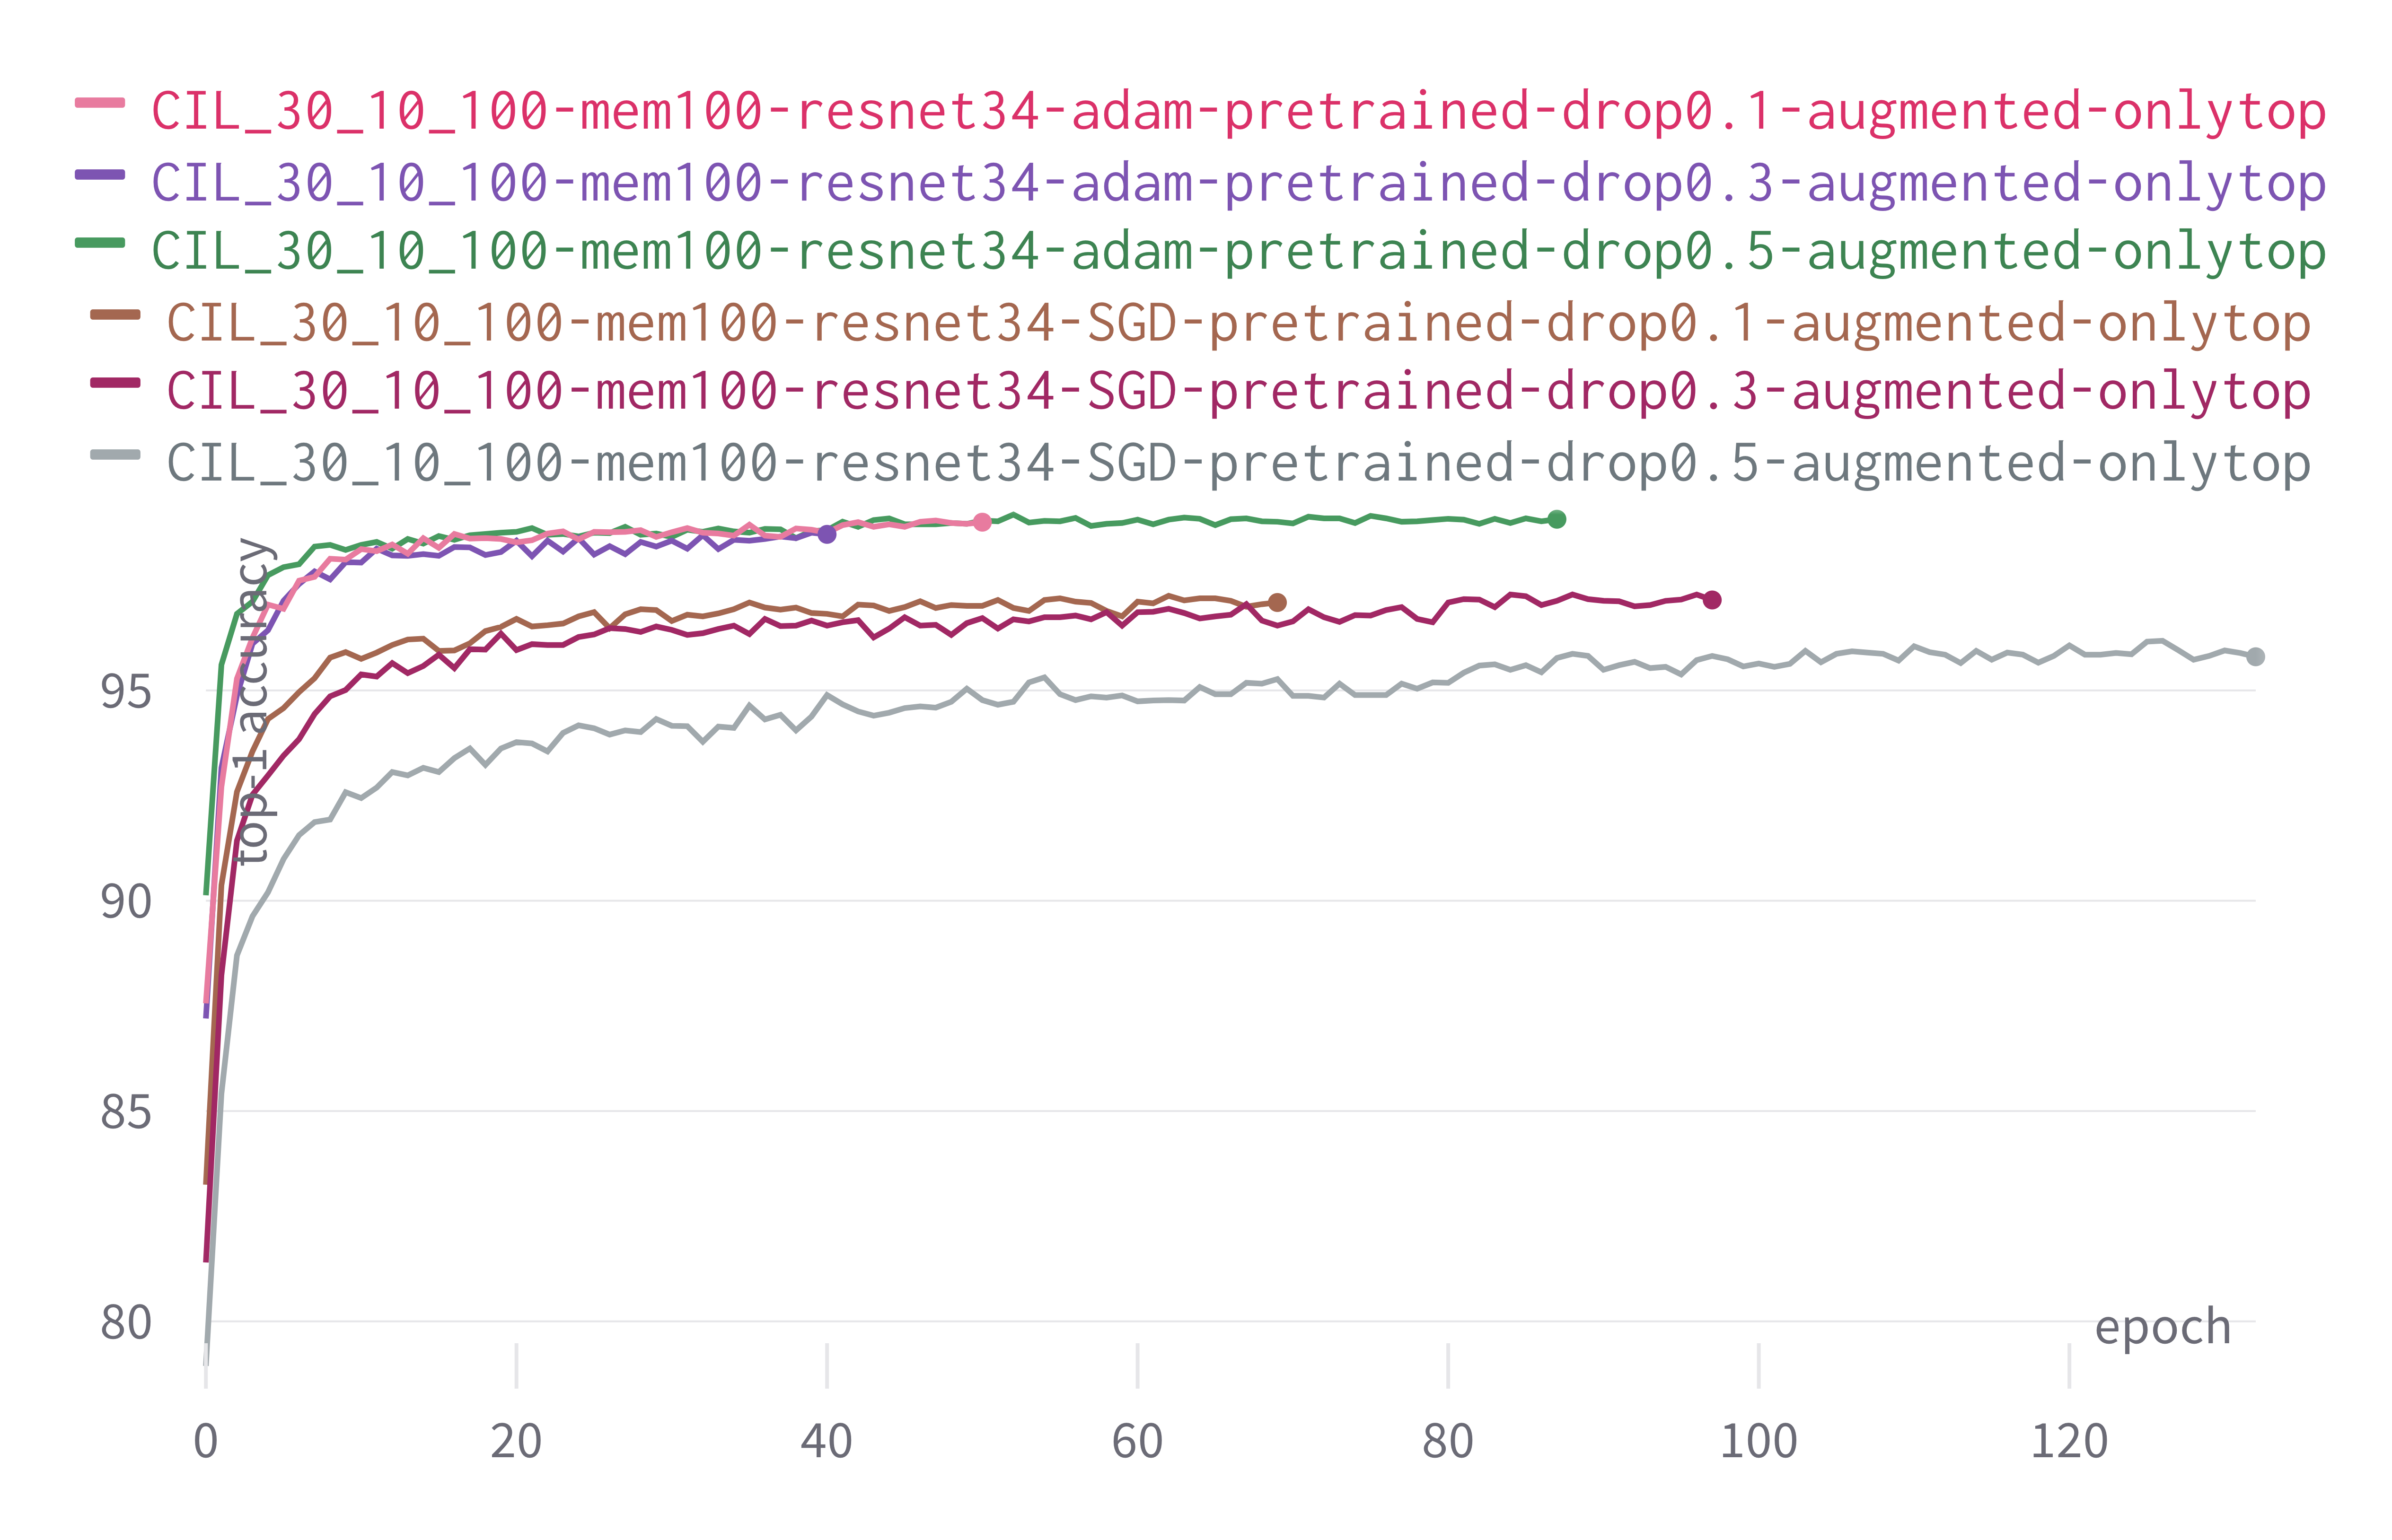
\includegraphics[width=0.80\textwidth]{images/exp/exp4-train.png} }}%
    \qquad
	\subfloat[\centering Accuracy on the validation set]{{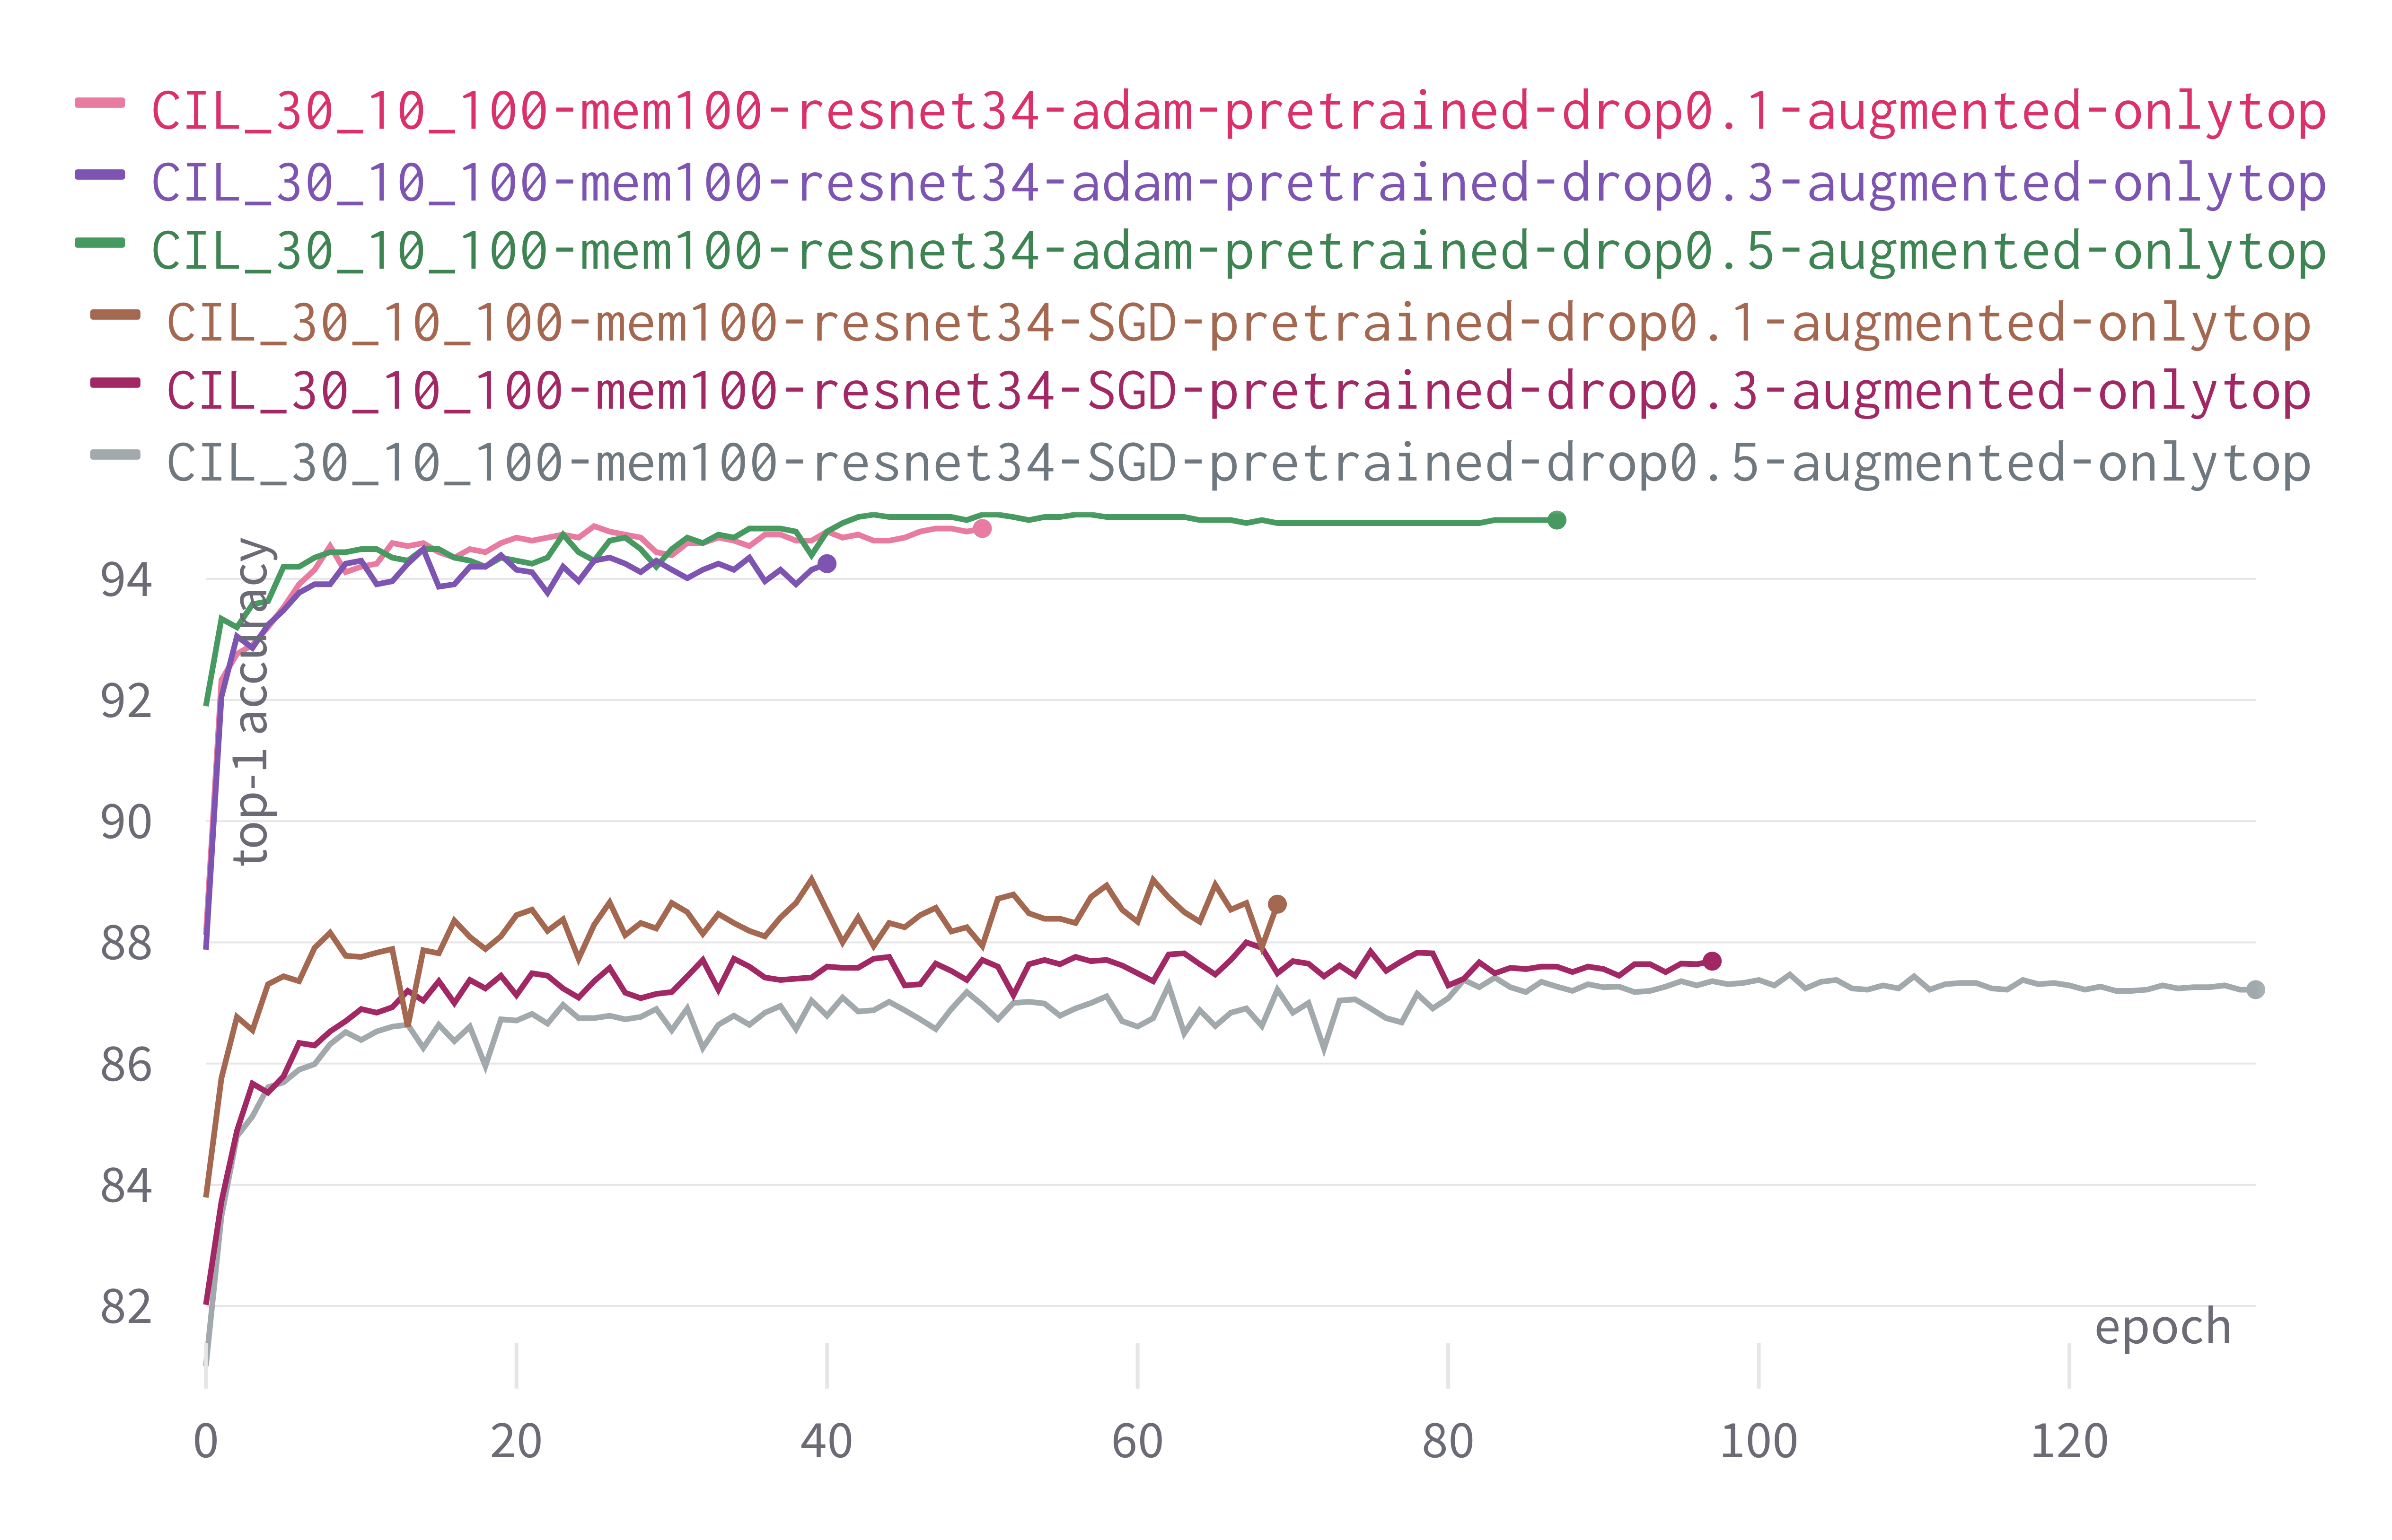
\includegraphics[width=0.80\textwidth]{images/exp/exp4-val.png} }}%
	\caption{Models trained using SGD and Adam: comparison of the accuracy at each training epoch at task 7 between the validation and training set.}%
	\label{fig:exp4-train_val}%
\end{figure}

\newpage


\newpage
\subsubsection{Type 2 baseline}
To address the problems relative to the type 1 baseline, the models tested in the previous section are compared to the 'type 2 baseline' described in \autoref{sec:method-baseline2}. This new baseline is trained on the same dataset used for CIL models and consists in fine-tuning ResNet-152 pretrained on ImageNet to the task of logo classification. This new baseline uses data augmentation, a dropout layer before the FC layer and the Adam optimizer.

Considering the top-1 and top-5 accuracy on the test set, the performance of CIL models and the type 2 baselines is compared in \autoref{table:baseline2}.
As we can see, the performance of the best CIL model is very similar to that of the baseline, but the latter still performs worse, even if slightly.
Although this new baseline mitigates the problem of the number of model parameters, this is still present, as shown in \autoref{table:baseline2-params}.

\begin{table}[H]
    \centering
    \centerline{
    \begin{tabular}{c|c|c}
        \hline
        \textbf{Model} &
        \textbf{Dropout} &
        \textbf{Top-1} \\
        \textbf{name} &
        \textbf{rate} &
        \textbf{acc. (\%)} \\
        \hline
\hline
adam-drop0.1-augmented-onlytop&0.1&92.15\\
adam-drop0.3-augmented-onlytop&0.3&91.55\\
adam-drop0.5-augmented-onlytop&0.5&\textbf{95.04}\\
\hline
BASELINE\_2-drop0.1-augmented-onlytop&0.1&82.35\\
BASELINE\_2-drop0.3-augmented-onlytop&0.3&94.11\\
BASELINE\_2-drop0.5-augmented-onlytop&0.5&88.23\\
\hline 
    \end{tabular}}
    \caption{Performance comparison between the CIL model and the type 2 baseline. Top-1 accuracy tested on 100 classes.}
    \label{table:baseline2}
\end{table}

\begin{table}[H]
    \centering
    \centerline{
    \begin{tabular}{c|c}
        \hline
        \textbf{Model} &
        \textbf{\#Params} \\
        \textbf{name} &
        \textbf{(M)} \\
        \hline
adam-drop0.1-augmented-onlytop&170\\
adam-drop0.3-augmented-onlytop&170\\
adam-drop0.5-augmented-onlytop&170\\
\hline
BASELINE\_2-drop0.1-augmented-onlytop&60\\
BASELINE\_2-drop0.3-augmented-onlytop&60\\
BASELINE\_2-drop0.5-augmented-onlytop&60\\
\hline 
    \end{tabular}}
    \caption{Number of model parameters between the CIL model and the typ 2 baseline.}
    \label{table:baseline2-params}
\end{table}

\newpage
\subsubsection{Type 3 baseline}
This third baseline, 'type 3 baseline' aims to solve the problem of the number of model parameters. In fact, this approach, described in \autoref{sec:method-baseline3}, defines the baseline architecture using the DER algorithm in the exact same setup as the CIL classifier, thus having an identical architecture of the CIL model and the baseline.
This ensures that the number of model parameters is the same.
Therefore, the baseline is trained using the same dataset, data augmentation, regularization, and the Adam optimizer.

The performance between the CIL models and this new baseline is compared considering the top-1 on the test set. As we can see from \autoref{table:baseline3}, the type 3 baseline achieves better performance than the CIL model.

This makes it possible to compare the actual drop in performance using an incremental learning setup compared to a standard setup.
As shown in \autoref{table:baseline3}, this gap is present, with a 3\% drop in top-1 accuracy, but it is expected using an incremental learning setup.
However, a 3\% drop is acceptable when considering the advantages of an incremental learning approach.

\begin{table}[H]
    \centering
    \centerline{
    \begin{tabular}{c|c|c}
        \hline
        \textbf{Model} &
        \textbf{Dropout} &
        \textbf{Top-1} \\
        \textbf{name} &
        \textbf{rate} &
        \textbf{acc. (\%)} \\
        \hline
\hline
adam-drop0.1-augmented-onlytop&0.1&92.15\\
adam-drop0.3-augmented-onlytop&0.3&91.55\\
adam-drop0.5-augmented-onlytop&0.5&95.04\\
\hline\
BASELINE\_3-drop0.1-augmented-onlytop&0.1&\textbf{98.52}\\
BASELINE\_3-drop0.3-augmented-onlytop&0.3&97.05\\
BASELINE\_3-drop0.5-augmented-onlytop&0.5&97.64\\
\hline 
    \end{tabular}}
    \caption{Top-1 accuracy of the CIL model and the type 3 baseline consider all the 100 classes of the test set.}
    \label{table:baseline3}
\end{table}

\newpage
\subsubsection{Pruning (100 classes)}
An important aspect discussed in \autoref{sec:method-pruning} is the number of model parameters. All the models tested up to this point add approximately 22 million parameters with each new incremental iteration of learning, thus reaching 170 million parameters at task 7 (22 million for the initial task and 7 iterations of incremental learning).

The following experiments are designed to assess the pruning capacity of the channel-level masks and the drop in performance obtained by using this method. To this end, the pruned models are compared to those described in the previous section. An important difference in the training procedure of the pruned model is to monitor the loss on the validation set instead of the validation accuracy. Since the validation loss decreases with increasing sparsity of the model, we want to encourage a sparser model given the same accuracy on the validation set.

The results regarding the performance comparison are shown in \autoref{fig:exp5} and \autoref{table:exp5}. As we can see, the drop in performance is negligible, with some pruned models performing even better than un-pruned ones. This can be explained by considering pruning as a regularization technique, in fact, the number of parameters reduced (effectively reducing the Vapnik-Chervonenkis dimension \cite{vapnik1999nature}). However, it is important to emphasize that these models are trained considering the top-100 classes, so it is essential to test the scalability of the models, and also of pruning, to the entire dataset.


\begin{figure}[H]
	\centering
	\subfloat[\centering Top-1 accuracy]{{\includegraphics[width=0.80\textwidth]{images/exp/exp5-top1.png} }}%
    \qquad
	\subfloat[\centering Top-5 accuracy]{{\includegraphics[width=0.80\textwidth]{images/exp/exp5-top5.png} }}%
	\caption{Performance comparison between the pruned model and standard model.}%
	\label{fig:exp5}%
\end{figure}

\begin{table}[H]
    \centering
    \centerline{
    \begin{tabular}{c|c|c|c|c}
        \hline
        \textbf{Model} &
        \textbf{Dropout} &
        \textbf{Pruning} &
        \textbf{Top-1} & 
        \textbf{Top-5} \\
        \textbf{name} &
        \textbf{rate} &
        &
        \textbf{acc. (\%)} & 
        \textbf{acc. (\%)} \\
        \hline
        \hline
drop0.1-augmented-onlytop&0.1&no&92.15&97.92\\
drop0.3-augmented-onlytop&0.3&no&91.55&97.75\\
drop0.5-augmented-onlytop&0.5&no&\textbf{95.04}&\textbf{98.4}\\
\hline
PRUNED-drop0.1-augmented-onlytop&0.1&yes&92.58&96.96\\
PRUNED-drop0.3-augmented-onlytop&0.3&yes&92.05&96.29\\
PRUNED-drop0.5-augmented-onlytop&0.5&yes&91.45&95.67\\
        \hline
    \end{tabular}}
    \caption{Performance comparison between the pruned models and the un-pruned ones. Top-1 accuracy at task 7.}
    \label{table:exp5}
\end{table}

The result of pruning regarding the number of parameters is shown in \autoref{fig:exp5-params} and \autoref{table:exp5-params}. As we can see, this technique is very effective. The final number of model parameters is reduced by almost a factor of 5x, the models not using pruning already exceed the total number of parameters of those using pruning for task 1 (43 for the un-pruned vs. 32 for pruned approx.).

\begin{table}[ht]
    \begin{minipage}[b]{0.49\linewidth}
        \centering
        \includegraphics[width=1\linewidth]{images/exp/exp5-params.png}
        \captionof{figure}{Number of model parameters at each task using the pruning technique.}
        \label{fig:exp5-params}
    \end{minipage}
    \hfill
    \begin{minipage}[b]{0.49\linewidth}
        \centering
        \begin{tabular}{c|c}
            \hline
            \textbf{Model} &
            \textbf{\#Params} \\
            \textbf{name} &
            \textbf{(M)} \\
            \hline
            \hline
UNPRUNED-drop0.1&170\\
UNPRUNED-drop0.3&170\\
UNPRUNED-drop0.5&170\\
\hline
PRUNED-drop0.1&34.08\\
PRUNED-drop0.3&32.48\\
PRUNED-drop0.5&36.41\\
            \hline
        \end{tabular}
            \caption{Number of model parameters at task 7.}
            \label{table:exp5-params}
    \end{minipage}
\end{table}

Other interesting insights emerge by analyzing the training history of the models at task 0. The loss function of the DER algorithm (\autoref{eq:final_der_loss}) is defined as the sum of: the loss of the classifier, the loss of the auxiliary classifier and loss related to the pruning masks. In \autoref{fig:exp5-loss} we can see the classification loss (c), the sparsity loss (d) and the final loss (b) of the model for each training epoch at task 0. Initially, the loss (c) tends to decrease, but as the training epochs advance, the sparsity loss (d) increasingly limits the channels of the convolutional layers. This leads to a continuous decrease in parameters, but the classification (c) is affected considerably. The deterioration in performance can also be seen in the top-1 accuracy (a) on the validation set.


\begin{figure}[H]
	\centering
	\subfloat[\centering Top-1 accuracy]{{\includegraphics[width=0.50\textwidth]{images/exp/exp5-val_acc.png} }}%
    
	\subfloat[\centering Final loss]{{\includegraphics[width=0.50\textwidth]{images/exp/exp5-val_loss.png} }}%
    
	\subfloat[\centering Classification loss]{{\includegraphics[width=0.50\textwidth]{images/exp/exp5-val_clf.png} }}%
    
	\subfloat[\centering Sparsity loss]{{\includegraphics[width=0.50\textwidth]{images/exp/exp5-val_spars.png} }}%
	\caption{Training history of the pruned model on the validation set at task 0.}%
	\label{fig:exp5-loss}%
\end{figure}


\subsection{2993 Classes}
\label{sec:whole_dataset_clf}

The following experiments test the scalability capabilities of the model. In fact, in this section, models will be trained on 2993 classes, i.e. the entire dataset.

\subsubsection{Varying the memory size}
Another important factor for testing the scalability of the model is the number of stored examples for old classes. Indeed, when many classes are introduced, it is necessary to limit the memory used to save old examples.
In this first section, the models are trained by varying the size of the memory used by the models to store examples of the old classes. The memory size is tested using: 50, 20 and 10 examples.

Regarding the other specifications of the model, it is trained according to the best results obtained previously with the experiments on 100 classes. Thus, the architecture of each feature extractor is ResNet-34 pretrained on ImageNet, the optimizer is Adam, regularization with a dropout layer is used as well as data augmentation, but initially no pruning is performed.

The results of the experiments are shown in \autoref{fig:exp6} and \autoref{table:exp6}.
As we can see, the models scale fairly well over the entire dataset, as a comparison of the setup of 100 classes shown in \autoref{table:exp5}, the drop in performance is only about 8\%, even though the examples stored in the setup of 2993 classes are 1/10 than before. As expected, the more samples stored for incremental learning iterations, the better the overall accuracy. The total number of examples stored by each model at task 8 is shown in \autoref{table:exp6-memsize}.

\begin{table}[H]
    \centering
    \centerline{
    \begin{tabular}{c|c|c|c|c}
        \hline
        \textbf{Model} &
        \textbf{Dropout} &
        \textbf{Mem.} &
        \textbf{Top-1} & 
        \textbf{Top-5} \\
        \textbf{name} &
        \textbf{rate} &
        \textbf{size} &
        \textbf{acc. (\%)} & 
        \textbf{acc. (\%)} \\
        \hline
        \hline
CIL\_2993-mem10-drop0.5-adam $\vardiamondsuit$ &0.1&10&87.2&92.19\\
CIL\_2993-mem20-drop0.5-adam&0.1&20&88.47&92.58\\
CIL\_2993-mem50-drop0.5-adam $\clubsuit$ &0.1&50&\textbf{89.22}&\textbf{92.97}\\
        \hline
    \end{tabular}}
    \caption{Performance of the models at each incremental task trained on the entire dataset using different dimensions of memory size. Top-1 accuracy at task 8.}
    \label{table:exp6}
\end{table}


\begin{table}[H]
    \centering
    \begin{tabular}{c|c|c}
        \hline
        \textbf{Model} &
        \textbf{Mem.} &
        \textbf{\# Total saved} \\
        \textbf{name} &
        \textbf{per class} &
        \textbf{examples (K)} \\
        \hline
        \hline
CIL\_2993-mem10-drop0.5-adam&10&102\\
CIL\_2993-mem20-drop0.5-adam&20&53\\
CIL\_2993-mem50-drop0.5-adam&50&29\\
        \hline
    \end{tabular}
    \caption{Number of total examples stored by each model at task 8.}
    \label{table:exp6-memsize}
\end{table}


\begin{figure}[H]
	\centering
	\subfloat[\centering Top-1 accuracy]{{\includegraphics[width=0.80\textwidth]{images/exp/exp6-top1.png} }}%
    \qquad
	\subfloat[\centering Top-5 accuracy]{{\includegraphics[width=0.80\textwidth]{images/exp/exp6-top5.png} }}%
	\caption{Performance of the models at each incremental task trained on the entire dataset using different dimensions of memory size.}%
	\label{fig:exp6}%
\end{figure}

\newpage

\subsubsection{Type 3 baseline (2993 classes)}
As in the case of 100 classes, the performance of the CIL models is compared with the type 3 baseline (see \autoref{sec:method-baseline3}). For this purpose, the baseline is trained considering the same dataset used to train the models in the previous section.
Note that in the case of the baseline, there is no need to use a memory for the old classes since the incremental learning setup does not hold.
 
The comparison of top-1 accuracy between CIL models and baselines is shown in \autoref{table:baseline3-2993}.
Osservazioni\todo{Osservazioni}


\begin{table}[H]
    \centering
    \centerline{
    \begin{tabular}{c|c|c|c}
        \hline
        \textbf{Model} &
        \textbf{Dropout} &
        \textbf{Mem.} &
        \textbf{Top-1}\\
        \textbf{name} &
        \textbf{rate} &
        \textbf{size} &
        \textbf{acc. (\%)} \\
        \hline
\hline
CIL\_2993-mem10-drop0.5-adam&0.1&10&87.2\\
CIL\_2993-mem20-drop0.5-adam&0.1&20&88.47\\
CIL\_2993-mem50-drop0.5-adam&0.1&50&89.22\\
\hline\
BASELINE\_3-2993classes-drop0.1&0.1&-&88.48\\
BASELINE\_3-2993classes-drop0.3&0.3&-&\textbf{91.92}\\
BASELINE\_3-2993classes-drop0.5&0.5&-&-\\
\hline 
    \end{tabular}}
    \caption{Top-1 accuracy of the CIL model and the type 3 baseline consider all the 100 classes of the test set.}
    \label{table:baseline3-2993}
\end{table}

\newpage

\subsubsection{Pruning (2993 classes)}
\label{sec:pruning-entire}
Similarly to the setup with 100 classes, the pruning strategy is tested for models trained on the entire dataset. As we can see from \autoref{fig:exp7} and \autoref{table:exp7}, when using the pruning in combination to the Weight Aligning (WA), the performance drops dramatically. Therefore, only for models using pruning, WA is disabled.

In contrast to the experiments on 100 classes, now pruning results in poor performance, in fact the drop in accuracy is considerable compared to those models without pruning. Even considering the case using 50 samples for the pruning model, performance deteriorates by almost 20\%.

Regarding the number of parameters, even in the setup with 2993 classes the model is reduced in size considerably. As we can see from \autoref{table:exp7-params}, however, the pruning factor corresponds to approximately 3x compared to the 5x achieved in the previous setup.

In conclusion, the pruning strategy is not effective in the case of models trained on the entire dataset. For this reason, the KD is used and the result of the experiments is shown in \autoref{sec:exp-kd}.

\begin{table}[H]
    \centering
    \begin{tabular}{c|c|c|c|c|c}
        \hline
        \textbf{Model} &
        \textbf{Mem.} &
        \textbf{WA} &
        \textbf{Pruning} &
        \textbf{Top-1} & 
        \textbf{Top-5} \\
        \textbf{name} &
        \textbf{size} &
        &
        &
        \textbf{acc. (\%)} & 
        \textbf{acc. (\%)} \\
        \hline
        \hline
UNPRUNED-WA-mem10-drop0.5&10&yes&no&87.2&92.19\\
UNPRUNED-WA-mem20-drop0.5&20&yes&no&88.47&92.58\\
UNPRUNED-WA-mem50-drop0.5&50&yes&no&\textbf{89.22}&\textbf{92.97}\\
\hline
PRUNED-noWA-mem10-drop0.3&10&no&yes&51.69&62.56\\
PRUNED-noWA-mem20-drop0.3&20&no&yes&63.2&73.97\\
PRUNED-noWA-mem50-drop0.3 $\spadesuit$&50&no&yes&70.37&81.85\\
\hline
PRUNED-WA-mem10-drop0.3&50&no&yes&7.6&10.67\\
\hline
\end{tabular}
\caption{Performance comparison between the pruned and un-pruned models. Top-1 accuracy at task 8.}
    \label{table:exp7}
\end{table}


\begin{table}[H]
    \centering
    \begin{tabular}{c|c}
        \hline
        \textbf{Model} &
        \textbf{\#Params} \\
        \textbf{name} &
        \textbf{(M)} \\
        \hline
        \hline
UNPRUNED-CIL\_2993-WA-mem10-drop0.5&205\\
UNPRUNED-CIL\_2993-WA-mem20-drop0.5&205\\
UNPRUNED-CIL\_2993-WA-mem50-drop0.5&205\\
\hline
PRUNED-CIL\_2993-noWA-mem10-drop0.3&68.79\\
PRUNED-CIL\_2993-noWA-mem20-drop0.3&71.66\\
PRUNED-CIL\_2993-noWA-mem50-drop0.3&68.33\\
\hline
PRUNED-CIL\_2993-WA-mem10-drop0.3&70.69\\
        \hline
    \end{tabular}
	\caption{Number of model parameters at task 8.}%
    \label{table:exp7-params}
\end{table}

\begin{figure}[H]
	\centering
	\subfloat[\centering Top-1 accuracy]{{\includegraphics[width=0.80\textwidth]{images/exp/exp7-top1.png} }}%
    \qquad
	\subfloat[\centering Top-5 accuracy]{{\includegraphics[width=0.80\textwidth]{images/exp/exp7-top5.png} }}%
	\caption{Performance comparison between the pruned and unpruned models trained on the entire dataset.}%
	\label{fig:exp7}
\end{figure}

\newpage

%\subsubsection{Ablation study}

\section{Knowledge Distillation}
\label{sec:exp-kd}
To address the drastic drop in accuracy when using pruning on models trained on the whole dataset (see \autoref{sec:pruning-entire}), KD is adopted as described in \autoref{sec:method-kd}. During the KD, an un-pruned model is used as the teacher, while the student is a significantly smaller CNN. In the experiments presented in this section, ResNet-50 pretrained on ImageNet is used as the backbone for the student, with a dropout layer before the FC layer.

KD is performed after the training of the teacher model. Since the CIL classifier is trained using the DER algorithm, and this algorithm requires that a part of the examples of the old classes is stored, in a real situation the KD can only be performed with those examples available as a result of the storage. For this reason, in order to reproduce a realistic situation, the student model is trained under the supervision of the teacher, but only the samples stored by the teacher are used as training data.

The result of the experiments regarding KD are shown in \autoref{table:exp-kd}, where different models with varying memory size are used as teachers. As we can see, the number of examples used to train the student heavily affects the final performance.
However, the student trained with 50 samples per class achieves 0.80 as top-1 accuracy, resulting in performance drop of 9\% compared to the teacher model. Although this drop in performance is rather large, it is important to consider the number of parameters: all teacher models have 205 million parameters, while the final models used as students have 30 million parameters.
Therefore, even if the accuracy drops, the number of parameters drops by a factor of almost 7x.

KD outperforms the result obtained with the pruning method (see \autoref{table:exp7} and \autoref{table:exp7-params}). In fact, comparing KD with pruning, the performance increases from 70.37\% to 80.0\% and the compression factor goes up from 3x to 7x.


\begin{table}[H]
    \centering
    \begin{tabular}{c|c|c|c|c}
        \hline
        \textbf{Teacher} &
        \textbf{Student} &
        \textbf{Mem.} &
        \textbf{Dropout rate} &
        \textbf{Top-1} \\
        \textbf{model} &
        \textbf{model} &
        \textbf{size} &
        \textbf{student} &
        \textbf{acc. (\%)} \\
        \hline
        \hline
UNPRUNED-WA-mem10-drop0.5&ResNet-50&10&0.1&62.42\\
UNPRUNED-WA-mem50-drop0.5&ResNet-50&10&0.3&69.09\\
UNPRUNED-WA-mem50-drop0.5 $\varheartsuit$&ResNet-50&50&0.3&\textbf{80.0}\\
\hline
\end{tabular}
\caption{Top-1 accuracy of the students trained using KD. The teacher column represents which model is used as teacher, the student column refers to the backbone of the student model. }
    \label{table:exp-kd}
\end{table}


\section{Logo detector}
\label{sec:exp-det}
This section described the experiments designed to evaluate the class-agnostic logo detector introduced in \autoref{sec:method-roi}.
The CIL classifier is trained starting from the cropped regions.
However, the detector predicts the bounding boxes using the entire image as input.
Since an image can contain multiple logos, the detector is trained to exploit the same training, validation and testing set used by the CIL classifier.
This is done by considering the training labels for the detector only if that bounding box corresponds to a ROI used as a training example for the classifier, otherwise the bounding box is used in the validation or test set, depending on the split used for the classifier.
This process is shown in \autoref{fig:detector-split-dataset}.
This results in an unbiased evaluation of both the detector and the classifier.

\begin{figure}[H]
	\centering
    \includegraphics[width=0.7\textwidth]{images/logos-split.drawio.png}
	\caption{Training, validation and test split for the detector based on the splits used to train the CIL classifier.}%
	\label{fig:detector-split-dataset}%
\end{figure}

\subsection{Metrics}
Mean Average Precision (mAP) metric is a metric used to evaluate object detection models. This metric is based on: Intersection over Union (IoU), Recall, Precision.

\subsubsection{Intersection over Union}
Given a ground-truth bounding box $box_{gt}$ and a detected bounding box $box_{pred}$, as shown in \autoref{fig:iou}, the IoU is computed as the ratio of the overlap and union areas:
\begin{equation}
    \text{IoU} = \frac{box_{gt} \cap box_{pred}}{box_{gt} \cup box_{pred}} 
\end{equation}
Then a prediction is considered correted if IoU $ \geq \tau$, where $\tau$ is a threshold (a typical value for $\tau$ is $0.5$).

\begin{figure}[H]
	\centering
    \includegraphics[width=1\textwidth]{images/iou.drawio.png}
	\caption{Intersection over Union (IoU). The green box represents the ground-truth bounding box, the red one represents the predicted bounding box and the intersection is given by the yellow region. Then, the IoU is computed as the ratio of the overlap and union areas.}
	\label{fig:iou}
\end{figure}

\subsubsection{Precision and Recall}
Given the IoU and a threshold $\tau$ it is possible to count the number of:
\begin{itemize}
    \item True Positive (\textbf{TP}): The number of bounding boxes which have a IoU $geq \tau$ with the ground-truth bounding box.
    \item False Positive (\textbf{FP}): The number of bounding boxes that predict an object which is not actually an object.
    \item False Negative (\textbf{FN}): The number of bounding boxes which have a IoU $< \tau$ with the ground-truth bounding box.
\end{itemize}
Note that the True Negative (TN) are not considered in an object detection task, as this would mean counting as TN the background of the image that contains no object.

Then, the Precision $P$ is given by:
\begin{equation} %tp / (tp + fp)
    P = \frac{TP}{TP + FP}
\end{equation}
and the Recall $R$ is given by:
\begin{equation} %tp / (tp + fn)
    R = \frac{TP}{TP + FP}
\end{equation}
Intuitively, precision is the ability of the detector not to consider as object a part of the image that is not, and recall is the ability of the detector to find all objects in the image.
The threshold $\tau$ affects the number of TP, FP, FN, thus the value of Precision and Recall. For this reason, given a value for $\tau$ (e.g. $\tau = 0.5$), when computing the Precision/Recall at $\tau = 0.5$, this is denoted by $P@.5$ and $R@.5$.

\subsubsection{Mean Average Precision}
Average Precision (AP) is calculated as the weighted mean of precisions at each threshold; the weight is the increase in recall from the prior threshold. For values of $\tau \in T$, where $T = [0.50, 0.55, 0.60,\, ..., \, 0.95 ]$, the AP computed using the thresholds in $T$ and denoted by $\text{AP}@.5:.95$ is given by:
\begin{equation}
    AP = 1 \sum_{i=1}^{|T| - 1}(R@\tau_i - R@\tau_{i+1} ) * P@\tau_{i}
\end{equation}
Finally, given $k$ different classes, the mAP is the average of the AP among each class:
\begin{equation}
    mAP = \frac{1}{k} \sum_{i=1}^{k} AP_i
\end{equation}

\subsection{100 Classes}

As described in \autoref{chap:methods}, the class-agnostic logo detector represents the first stage of the system and works in combination with the CIL model to achieve incremental learning logo detection and recognition.

\subsubsection{Training using the 30 classes of the initial task}
Similarly to the CIL classifier, the first logo detector experiments focus on the the top-100 classes of the dataset (where top-100 refers to the 100 classes with the highest number of samples, see \autoref{sec:cil-top100}).
Given the nature of the problem, in a real case scenario, the detector is trained using only those classes available for the CIL model at task 0. In the experimental setup described in \autoref{sec:exp-setup}, the initial task consists of 30 classes.

For this reason, in the top-100 classes setup, the detector is trained for 30 epochs with the SGD optimizer using only those 30 classes available at task 0.
Note that, as described before, the 30 classes correspond to those considered by the CIL model at task 0. Furthermore, the train, validation and test sets for the detector are maintained identical as the classifier, so that to use the same sample images for training and testing of the two models

During the training of the detector, the object loss, box loss (see \autoref{sec:yolo} and \autoref{eq:yolo-loss}) and the mAP@.5 is monitored on the validation set. The performance shown in \autoref{fig:exp-det_100} considers only the 30 classes used for training, which is a useful information for analyzing the training phase. However, considering an incremental learning setup, we expect the class-agnostic logo detector to perform well on all the 100 classes.
To this purpose, the detector is evaluated considering the mAP@.5 on the test set of the initial 30 classes and the test of the remaining 70 classes.
This evaluation represents a real-world scenario and it is therefore the most reliable performance and best suited to assessing the detector.
The result of the evaluation is shown in \autoref{table:exp-det_100}.


\subsubsection{Generalization capabilities of the class-agnostic logo detector}
To better investigate the generalizing capabilities of the detector trained on 30 classes to the remaining 70, the detector is compared with a new one trained on all the 100 classes.
This detector can be considered as a baseline with regard to the generalization capabilities of the detector trained on 30 classes: the smaller the gap between the performance of these two models, the better the generalization capabilities.
This new detector is trained for 30 epochs on the 100 classes and, as before, the object loss, box loss and the mAP@.5 is monitored on the validation set. The comparison between the two detector is shown in \autoref{fig:exp-det_100}.

As we can see from \autoref{fig:exp-det_100}, the performance between the detectors trained on 100 and 30 classes are quite similar. However, a crucial aspect of this training results, is that these metrics consider all and only the classes which the model is trained on, thus 30 classes and 100 classes.
The fact that the detectors achieve the same performance is a sign that they accomplish similar results in detecting logos across a different number of classes.
However, the real comparison consists in considering the mAP@0.5 for each detector, computed on the test set of all the 100 classes. This comparison is shown in \autoref{table:exp-det_100}.

From \autoref{table:exp-det_100}, we can see how the detector trained on 30 classes does not generalize well on the remaining 70 classes.
In fact, comparing the mAP@.5 computed on the test set composed of all the 100 classes, with the mAP@.5 obtained on the validation in the last epochs of training (shown in \autoref{fig:exp-det_100}), the drop in performance goes from about 0.97 to 0.75.

In contrast, the detector trained on all the 100 classes, obtains a mAP@.5 on the test set of 0.982, which is consistent with the performance obtained on the validation set in the last epochs of training.
However, it must be considered that, as this detector is trained using 70 more classes, it has more training samples at its disposal, hence more data from which to acquire knowledge of a logo.


\begin{table}[H]
    \centering
    \begin{tabular}{c|c|c|c|c}
        \hline
        \textbf{Model} &
        \textbf{Precision} &
        \textbf{Recall} &
        \textbf{mAP@.5} &
        \textbf{mAP@.5:.95} \\
        \hline
        \hline
DET\_class-agnostic\_30cls&0.784&0.659&0.75&0.542\\
DET\_class-agnostic\_100cls&0.944&0.972&0.982&0.776\\
\hline
\end{tabular}
\caption{Precision, Recall, mAP@.5 and mAP@.5:.95 obtained by the detector trained on 30 classes (DET\_class-agnostic\_30cls) and that trained on 100 classes (DET\_class-agnostic\_10cls). The performance refers to the test set composed of all the 100 classes.}
    \label{table:exp-det_100}
\end{table}
\newpage

\begin{figure}[H]
	\centering
	\subfloat[\centering mAP@.5]{{\includegraphics[width=0.70\textwidth]{images/exp/exp-det-map.png} }}%
    \qquad
	\subfloat[\centering Box loss]{{\includegraphics[width=0.70\textwidth]{images/exp/exp-det-box_loss.png} }}%
    \qquad
	\subfloat[\centering Object loss]{{\includegraphics[width=0.70\textwidth]{images/exp/exp-det-obj_loss.png} }}%
    \caption{Performance comparison between the class-agnostic logo detector trained on 30 classes and the one trained on 100 classes. The plots show the mAP@.5, box loss and object loss on the validation set at each training epoch. Note that these performance are computed on the validation set of each model, thus using 30 and 100 classes respectively.}%
	\label{fig:exp-det_100}
\end{figure}


\subsection{2993 Classes}
\label{sec:2993-detector}
The experiments conducted in the previous section are performed in the same way for the 2993 classes setup.
The 2993 classes setup (see \autoref{sec:exp-setup}) consists of 1000 classes used at the initial task, then at each incremental task 250 classes are added.
This section evaluates how the detector's ability to scale when going from the recognition of 100 classes to the case of 2993 classes.

As in the case for the top-100 classes setup, the detector is trained on the first 1000 classes of the initial task, then the evaluation metrics are computed on the test set of these 1000 classes combined with the remaining 1993, thus the entire dataset consisting of 2993 classes in total.

The detector is trained for 30 epochs with the SGD optimizer using only those 1000 classes available at task 0.
During the training, the object loss, box loss (see \autoref{sec:yolo} and \autoref{eq:yolo-loss}) and the mAP@.5 is monitored on the validation set composed of the 1000 classes used for training.
As we can see in \autoref{fig:exp-det_2993}, the mAP@.5 of the model computed on the validation set is lower than the 30 or 100 classes setup.
This result is self-explanatory, as recognizing 1000 different logos is a more difficult task than recognizing 30 or 100 different logos.

Other than the performance on the validation set during the training, the most useful insights are obtained when evaluating the detector on the test set composed of all the 2993. The result is shown in \autoref{table:exp-det_2993}.

Another important comparison is between the detector trained on 1000 classes and the one trained on all the 2993 classes, as done for the 100 classes setup.
This is done to asses the generalization capabilities obtained by the detector trained on 1000 classes when tested on all the classes. The training result of the detector trained on 2993 classes is shown in \autoref{fig:exp-det_2993} and the final performance obtained when testing the detector on the entire dataset in shown in \autoref{table:exp-det_2993}.

OSSERVAZIONI\todo{osservazioni}
From the performance obtained in \autoref{table:exp-det_100} we can see how the gap in mAP@.5 between the detector trained on 30 classes and the one trained on 100 classes in quite large. However, from the results obtained in \autoref{table:exp-det_2993} emerges that, unlike the previous setup, this gap in mAP@.5 reduces. This is a key observation since this is an evidence that, indeed, the detector trained on 1000 classes is able to generalize well, hence detects the the remaining 1993 classes even if it is trained only on the first 1000 classes.

This result is a fundamental aspect for the entire system, as it is evidence in support of the claim made in \autoref{chap:introduction}, where it is assumed that it is not necessary to also develop an incremental learning detector, since the idea of what a generic logo is can be learned and well approximated using only an initial set of logos. The subsequent creation of new logos will not disrupt the general idea of a logo.

\begin{table}[H]
    \centering
    \begin{tabular}{c|c|c|c|c}
        \hline
        \textbf{Model} &
        \textbf{Precision} &
        \textbf{Recall} &
        \textbf{mAP@.5} &
        \textbf{mAP@.5:.95} \\
        \hline
        \hline
DET\_class-agnostic\_1000cls&0.704&0.666&0.706&0.465\\
DET\_class-agnostic\_2993cls&-&-&-&-\\
\hline
\end{tabular}
\caption{Precision, Recall, mAP@.5 and mAP@.5:.95 obtained by the detector trained on 1000 classes (DET\_class-agnostic\_1000cls) and that trained on 2993 classes (DET\_class-agnostic\_2993cls). The performance refers to the test set composed of all the 2993 classes.}
    \label{table:exp-det_2993}
\end{table}
\newpage

\begin{figure}[H]
	\centering
	\subfloat[\centering mAP@.5]{{\includegraphics[width=0.70\textwidth]{images/exp/exp-det-map.png} }}%
    \qquad
	\subfloat[\centering Box loss]{{\includegraphics[width=0.70\textwidth]{images/exp/exp-det-box_loss.png} }}%
    \qquad
	\subfloat[\centering Object loss]{{\includegraphics[width=0.70\textwidth]{images/exp/exp-det-obj_loss.png} }}%
    \caption{Performance comparison between the class-agnostic logo detector trained on 1000 classes and the one trained on 2993 classes. The plots show the mAP@.5, box loss and object loss on the validation set at each training epoch. Note that these performance are computed on the validation set of each model, thus using 1000 and 2993 classes respectively.}%
	\label{fig:exp-det_2993}
\end{figure}


\section{End to end classification}
\label{sec:exp-end2end}

In this last section, the whole system is tested. This consists in combining the two steps (see \autoref{chap:methods}): the class agnostic logo detection which generates ROIs, and the actual classification performed by the CIL classifier.
Then, the final performance is evaluated considering the Precision, Recall, mAP@.5 and mAP@.5:.95 on the test set composed of all the 2993 classes.

The model used for the first step of the system is the class agnostic logo detector presented in \autoref{sec:2993-detector} which is trained using only the 1000 classes used at task 0 by the CIL classifier.
This is done to replicate a real scenario.

For what concerns the CIL classifier the following models are compared:
\begin{enumerate}
    \item CIL classifier with memory 50 ($\clubsuit$ in \autoref{table:exp6}).
    \item CIL classifier with memory 10 ($\vardiamondsuit$ in \autoref{table:exp6}).
    \item CIL classifier with memory 50 pruned using learnable masks ($\spadesuit$ in \autoref{table:exp7}).
    \item Student model trained with KD by the CIL classifier with memory 50 ($\varheartsuit$ in \autoref{table:exp-kd}).
\end{enumerate}

The result of this evaluation is shown in \autoref{table:exp-end2end}. Osservazioni\todo{Osservazioni}.

\begin{table}[H]
    \centering
    \begin{tabular}{c|c|c|c|c}
        \hline
        \textbf{CIL classifier} &
        \textbf{Precision} &
        \textbf{Recall} &
        \textbf{mAP@.5} &
        \textbf{mAP@.5:.95} \\
        \hline
        \hline
CIL\_classifier-mem50 $\clubsuit$&0.578&0.615&0.614&0.417\\
CIL\_classifier-mem10 $\vardiamondsuit$&0.545&0.591&0.583&0.397\\
Pruned\_CIL\_classifier-mem\_50 $\spadesuit$&0.496&0.485&0.489&0.347\\
KD\_classifier-mem\_50 $\varheartsuit$&0.558&0.604&0.59&0.403\\
\hline
\end{tabular}
\caption{End-to-end performance of the system using the class-agnostic logo detector and different CIL classifiers. The Precision, Recall, mAP@.5 and mAP@.5:.95 are computed on the test set composed of all the 2993 classes.}
    \label{table:exp-end2end}
\end{table}

\chapter{Conclusions and future works}
\label{chap:conclusions}

This thesis addressed the task of logo recognition by reformulating the problem in a class incremental learning approach.
The motivation behind the use of this technique is that new logos are continuously being created.
Consequently, an effective model should be able to keep up with the introduction of new logos in order to recognize them, without the need to retrain a model but rather by integrating old knowledge with new one.

To this end, a two-stage logo detector is used to solve the problem, which consists of a first stage relating to the localization of logos in the image and a second stage regarding the actual classification of logos.

The first stage consists in a class-agnostic logo detector (i.e. the logo detector identifies any type of logo, without recognizing the specific class), in this way it is possible to decouple localization from recognition, thus avoiding the need to create a Class Incremental Learning (CIL) logo detector. 
This approach proves to be successful, as a generic logo detector is able to learn what a logo is by using only an initial set of logos.
The logo detector is then capable of generalizing and detect previously unseen logos.

On the other hand, taking advantage of state-of-the-art incremental learning techniques, a CIL classifier is defined to accomplish the actual classification of logos, using the Regions of Interest (ROIs) provided by the agnostic logo detector.
Experiments show that a classifier trained in this fashion, storing 50 examples of old classes, performs well without significant drawbacks in terms of performance compared to a standard approach (according to the results of the baseline comparison).

A downside of the algorithm used for CIL is the number of model parameters.
The method implemented with learnable masks used to perform channel-level pruning of the Convolutional Neural Network (CNN) layers achieves promising performance when tested on a subset of the dataset.
However, this approach performs poorly when trying to scale to the entire dataset.
To solve this problem, Knowledge Distillation is used as an alternative approach to channel-level masks.
In this way, it is possible to train a significantly smaller CNN with the supervision of a larger model resulting from the incremental learning steps.
Note that, in the experiments conducted in this thesis, the Knowledge Distillation (KD) is applied at the end of all incremental learning tasks, however the Dynamically Expandable Representation (DER) algorithm \cite{yan2021dynamically} is flexible enough to be used in combination with KD.
In the case where there is a need to recognize new logos after the KD (given the incremental learning nature of the problem), it would be possible to exploit the student architecture resulting from the KD, instead of the initial teacher model.
It would be sufficient to freeze the student weights trained with the KD and then expand the architecture with the DER algorithm for subsequent incremental learning iterations, like any other type of feature extractor in the standard DER configuration.
However, this is true from a theoretical point of view and further experiments should be conducted to verify the effectiveness of this technique and evaluate its performance.

The final performance obtained by the proposed approach is tested on the LogoDet-3K dataset.
The results show how, considering the class-agnostic logo detector trained on 1000 classes and the CIL classifier trained using KD, the proposed approach outperforms the end-to-end model proposed by the authors of LogoDet-3K \cite{wang2022logodet}.
On the other hand, the model proposed by Amazon in SeeTek \cite{li2022seetek} performs better on the LogoDet-3K dataset. However, it should be taken into account that SeeTek considers an open-set retrieval environment as opposed to an incremental learning setup considered in this thesis.
Furthermore, from the final results obtained by the proposed system emerge that the class-agnostic logo detector acts as a bottleneck for the whole system, thus severely limiting the final performance.

Future improvements of this work could tackle the problem related to the class-agnostic logo detector by considering a version of the YOLO detector \cite{glenn_jocher_2021_5563715} with a higher number of parameters and a larger input image size.
However, this would lead to higher computational requirements to train the model as well as longer training and inference times.
Another way to address this problem is to experiment with different architectures for the detector.
Additional improvements of the system are related to the second stage of the pipeline performed by the CIL classifier.
The classification task could be improved by enriching the representation of each logo by considering the textual component in addition to the visual feature.
This approach adopted in the literature is very effective, since many logos have a text component that can be used to distinguish them.
Further studies can be conducted in the direction of explainability, which is a hot topic in artificial intelligence when using deep learning models. This research could investigate what the detector considers as logos and explain why such detection applies to a given input.

\appendix
% INCLUSIONE APPENDICI - - PERSONALIZZARE - TENERE COERENTE CON LISTA IN ALTO
\chapter{An appendix}
\label{app:a}
% DA RIMUOVERE - LOREM IPSUM PER DIMOSTRAZIONE
%\foreignlanguage{english}{\Blindtext}


%%%%%%%%%%%%%%%%%%%%%%%%%%%%%%%%%%%%%%%%%%%%%%%%%%%%%%%%%%%%%%%

% BIBLIOGRAFIA
\phantomsection
\addcontentsline{toc}{chapter}{\refname}
\nocite{*}
\printbibliography

\end{document}
